% ===========================
% # Relatório de Atividades #
% ===========================

\part{Relatório de Atividades}

\section{Introdução}

Ao longo do mandato 2017/2018, o \acrshort{neeec}, realizou mais de uma centena de iniciativas, um número recorde na nossa casa e caso raro numa estrutura deste tipo, constituída por voluntários numa causa comum. Desta forma, achamos essencial deixar, de forma escrita, um relato das atividades realizadas, do feedback das mesmas e tentar relatar os pormenores que levaram ao sucesso das mesmas e os pormenores em falta para que o \acrshort{neeec} seja uma instituição feita de progresso e não de avanços e recuos. Assim, nesta secção, apresentamos as várias atividades realizadas pelo \acrshort{neeec} ao longo deste mandato, divididas pelas respetivas áreas.

\clearpage
% ========================
% # Geral                #
% ========================

\section{Geral}

\subsection{Introdução}

Ao longo do mandato, existiram inúmeras atividades/iniciativas que não pertenciam a um pelouro em específico mas sim ao \acrshort{neeec} no geral. Estas atividades eram, por regra, orientadas pela Direção mas a sua realização dependia, largamente, da participação de todos os membros do Núcleo, desde coordenadores a colaboradores.

\subsection{Atividades}

% ========================
% # Ação Social          #
% ========================

\subsubsection{Ação Social}

\paragraph{Doação aos Bombeiros}

Aquando dos incêndios do verão de 2017 gerou-se em Portugal uma onda solidária que tinha como objetivo a doação de alimentos aos bombeiros que combatiam os incêndios. Esta foi uma campanha que rapidamente se alastrou a toda a comunidade. O \acrshort{neeec} divulgou então a sua disponibilidade para receber bens na sala do Núcleo. Contudo, provavelmente devido aos já elevados pontos de recolha, a campanha quer em junho, quer em outubro foi um fracasso.

Em dezembro decidimos dedicar o mês solidário à causa dos incêndios tendo angariado bens alimentares, bens materiais e dinheiro. Os bens alimentares e materiais acabaram por ter de se doar à Casa de Infância Elísio de Moura, como é costume noutros anos, uma vez que as quantidades já angariadas para a causa dos incêndios era demasiado grande. Por sua vez, o dinheiro angariado no lanche solidário foi doado a um fundo dedicado ao apoio à reabilitação das áreas agrícolas destruídas.

Para esta campanha, foram instalados caixotes na entrada do \acrshort{deec}, no piso 2, na zona do bar e na sala de convívio. A campanha foi muito divulgada junto dos professores. Todas as atividades de dezembro tinham também entrada gratuita acompanhada da necessidade de se doar um bem alimentar. Desta forma, conseguiu-se uma recolha muito expressiva sendo necessário um carro completamente cheio para transportar os bens.


\paragraph{The Street Store}

Como é habitual todos os anos, a \acrfull{dg} e a \acrfull{sddh} realizaram mais uma edição "The Street Store" onde durante um fim de semana, num conceito muito semelhante a uma loja vulgar, disponibilizaram roupa, calçado, refeições, cuidados de higiene, alguns serviços, entre outras coisas, a população sem-abrigo e carenciada da cidade de Coimbra, proporcionando, também, momentos de convívio e entretenimento.

Dessa forma, solicitaram a ajuda dos núcleos de estudantes para a recolha de bens para a mesma. Desta forma, o \acrshort{neeec} aceitou o convite bastando para isso fazer a habitual divulgação e colocar os caixotes na zona do bar, entrada do \acrshort{deec} e sala de convívio, à semelhança das restantes campanhas solidárias feitas ao longo do ano.

De notar que para obtermos uma maior recolha de bens, enviámos email para os professores sensibilizando-os da campanha em questão. Foram preenchidos cerca de quatro caixotes, sendo que no último dia da campanha membros da \acrshort{dg} vieram ao Núcleo recolher os mesmos. O \acrshort{neeec} cedeu ainda alguns bens alimentares resultantes de sobras de febradas e afins que já não deveriam ser utilizados nas próximos eventos, dado os seus prazos de validade, mas que eram ainda bons para a altura em que se iria realizar a Street Store.

Esta é, sem dúvida, uma atividade que recomendamos o \acrshort{neeec} a participar.


% ========================
% # AAC (in)Forma        #
% ========================

\subsubsection{AAC (in)Forma}

Todos os anos a \acrshort{dg} leva a cabo sessões que têm como objetivo formar os núcleos de estudantes recém-empossados para o trabalho a levar a cabo durante o ano.

No ano de 2017, a \acrshort{dg} organizou o \acrshort{aac} (in)Forma em duas sessões, iguais, numa sexta-feira e num sábado (30 de junho e 1 de julho, respetivamente) sendo que os elementos dos NE’s podiam ir às sessões dos temas que lhes interessavam em qualquer um dos dois dias. Após votação no \acrshort{cin} anterior, a sessão de sexta-feira decorreu no Departamento de Física e a sessão de sábado decorreu no Departamento de Mecânica (ambos os departamentos foram propostos pelos NE’s que deles tomam conta pelo que, em futuras edições, caso funcione da mesma forma, o \acrshort{deec} poderá albergar este evento caso o \acrshort{neeec} se disponha a tal na \acrshort{an}).

As sessões propostas pela \acrshort{dg} para este \acrshort{aac} (in)Forma foram as seguintes:
\begin{itemize}
\item Política Educativa
\item Órgãos de Governo
\item Ação Social
\item Administração e Tesouraria
\item \acrshort{gape}
\item Pedagogia
\item Saídas Profissionais
\item Relações Externas
\item Cultura
\item Desporto
\item Relações Internacionais
\item Comunicação e Imagem
\item Intervenção Cívica
\item Novos Estatutos da \acrshort{aac}
\end{itemize}

Após o CIN, a Direção do \acrshort{neeec} informou de imediato os seus CGs para que estes investigassem junto das suas equipas sobre quem queria ou não ir às sessões, não exigindo nenhum mínimo de presenças sobre estes mas insistindo na importância de ter, pelo menos, os CGs presentes. Alguns pelouros, nomeadamente a Pedagogia, tiveram uma adesão enorme à atividade indo quase toda a equipa à sessão da Pedagogia e mais de metade da mesma à sessão do \acrshort{gape}, mas tal não se verificou muito nas restantes sessões. Estiveram presentes nas sessões das áreas que representam os CGs da Pedagogia e \acrshort{gape}, das Relações Externas e Comunicação, da Cultura e Lazer e da Imagem e ainda o Presidente e o Secretário da Mesa do Plenário. A CG das Saídas Profissionais e Formação não pode estar presente, mas assegurou de imediato a presença de um dos seus Coordenadores, enquanto que o CG do Pelouro do Desporto não esteve presente nem providenciou ninguém para estar presente. O Administrador do Núcleo também não esteve presente na sessão da sua área não tendo providenciado ninguém do seu Pelouro para o substituir, baseando-se na presença dos restantes elementos da Direção para lhe transmitir a informação. Da Direção do Núcleo, o Presidente, o Vice-Presidente e o Tesoureiro estiveram presentes em todas as sessões (exceto quando estas eram sobrepostas em que estes tiveram de se dividir entre si).

Quanto às sessões no geral, o tempo e qualidade das mesmas bem como o facto da orgânica da \acrshort{dg} não ser exatamente igual à do \acrshort{neeec} não possibilitam que este evento sirva, nem de perto nem de longe, como evento único de formação para os elementos do \acrshort{neeec}. Acontece ainda que existem sessões muito boas, como a da Comunicação, na qual não esteve presente o CG da área em questão pelo que este perdeu uma oportunidade de formação, e sessões, como a das Saídas Profissionais, de muito fraca qualidade não permitindo qualquer tipo de formação aos elementos que estiveram presentes. Por sua vez, temas como os órgãos de governo, em que quase nenhum elemento do \acrshort{neeec} sabe do assunto, não têm adesão pelo que o tema continua sem ser sabido pela equipa. Por sua vez, de notar que a sessão sobre os estatutos da \acrshort{aac} foi de elevada qualidade e foi fulcral quer para a Direção bem como para a Mesa do Plenário poderem aplicar os estatutos nos diversos regulamentos que tiveram de redigir, aumentando assim a qualidade dos regulamentos redigidos e também a real e fácil aplicação dos mesmos à orgânica do \acrshort{neeec}.

Posto isto, a nossa sugestão para o futuro é:
\begin{itemize}
\item Manter a presença do \acrshort{neeec} neste tipo de eventos e garantir a presença obrigatória quer dos CGs, quer dos Colaboradores.
\item Elaborar formações internas (profundas e aplicadas à orgânica do \acrshort{neeec}) sobre estes temas logo no início do mandato para que todos os elementos do \acrshort{neeec} possam saber as informações.
\item Incentivar as diversas equipas do \acrshort{neeec} a tomar conhecimento dos temas das outras equipas de forma a que estas percebam que as equipas do \acrshort{neeec} não são isoladas entre si e que entendam a orgânica do \acrshort{neeec}.
\item Relatar/relembrar à \acrshort{dg}, antes do início das edições deste tipo de eventos, o que correu mal na(s) última(s) para que se evite voltar a ter sessões sem qualidade.
\end{itemize}


% =========================
% # Semana das Matrículas #
% =========================

\subsubsection{Semana das Matrículas}

Durante a semana das matrículas, organizada pela \acrshort{uc} em conjunto com a \acrshort{aac}, os núcleos (e outras organizações como, por exemplo, o BEST) têm uma banca no Átrio das Químicas, junto à Faculdade de Medicina do Polo 1. No caso dos núcleos, os caloiros, teoricamente, são encaminhados, no final do processo de matrícula, para a banca do Núcleo que diz respeito ao seu curso. É de notar, que este processo não ocorre da forma mais ordeira pelo que muitos dos caloiros visitam a banca antes de entrarem no processo de matrículas e outros (muitos) saem do processo de matrículas e já não se dirigem à banca do Núcleo pois estão cansados ou querem ir embora com medo das praxes que poderão ser sujeitos. É também de realçar que, cada vez mais, os estudantes matriculam-se na internet não indo à banca das matrículas.

Para assegurar a gestão da banca do \acrshort{neeec} foi criada uma escala para todos os dias com início às 8h45 e término após as 17h. De notar que no primeiro dia a hora para montagem das bancas era às 7h45, horário esse que não foi cumprido pelo \acrshort{neeec}, e ainda bem, uma vez que pelas 9h, hora em que chegámos, as bancas ainda não estavam no Átrio, disponíveis para ser montadas. Após o primeiro dia, as mesas e cadeiras ficam no átrio das químicas pelo que é apenas recolhido todo o material das bancas que pode ser levado ou pode ficar guardado no \acrshort{nedf}. De realçar que o espaço é bastante ventoso pelo que é necessário prender muito bem o roll up do Núcleo para este não voar nem se estragar. Este ano, fizemos um formulário auxiliar que permitia aos Colaboradores presentes na banca fazerem um questionário seguido aos caloiros. Nesse formulário, era questionado o nome do caloiro (havia uma lista com todos aqueles que entraram na 1ª fase), eram explicadas as informações sobre a comunicação do \acrshort{neeec} (Facebook, Instagram e site. Recomendava-se ainda uma visita ao Facebook do Somos Polo 2. De seguida, explicava-se o programa das semanas de receção ao caloiro e era entregue um flyer aos caloiros com todo o programa destas semanas. Nesta apresentação, aproveitou-se para apresentar as \acrshortpl{rga} e a \acrshort{f3e}, atividades importantes mas não tão direcionadas para os caloiros, de forma a que estes fossem tomando uma ideia do que o \acrshort{neeec} fazia. De seguida, era apresentado o jantar de curso estando já abertas as inscrições. Desta forma, os pais podiam logo apoiar financeiramente a inscrição do evento. Era também apresentada a Latada. Por fim, davam-se mais alguns papeis com informações úteis como um mapa do Polo 2, uma pequena explicação sobre as cantinas, bares e residências dos \acrshort{sasuc}, um mapa do \acrshort{deec}, os horários dos SMTUC para as linhas 34 e 38. Era também apresentada de novo a \acrshort{aac} (os caloiros já passam por uma banca da \acrshort{aac} no interior do circuito). Este ano existia também uma grelha da \acrshort{dg} sobre Desporto Universitário que deveria ser preenchida pelos caloiros. Por fim, falava-se da praxe tentando acalmar qualquer medo que houvesse. Para finalizar, era apresentado o mega convívio do polo 2 e tentava-se fazer a venda de pulseiras para o evento (aqui, muitos doutores falavam negativamente do evento prejudicando a venda das pulseiras, o que é de evitar de todo).

Este novo modelo da banca correu bastante bem tendo a impressão do material sido positiva pois os caloiros, ao levarem com tanta informação, absorvem muito pouco pelo que, ao levarem os papéis, podem “rever a matéria em casa”. A implementação de um inquérito online também foi muito útil e conduziu os membros do Núcleo a fazer as questões corretas aos caloiros. Nota-se também uma taxa muito mais elevada de respostas comparando com o questionário escrito à mão e não há qualquer problema com a “descodificação de letras”. Há, no entanto, dois problemas a referir: o primeiro é o facto da internet (quer por wifi, quer por dados móveis) ser fraquíssima naquele local e nem toda a gente ter dados móveis, o que dificultou, às vezes, o preenchimento e o facto de algumas pessoas preferirem fazer as suas próprias questões pela ordem que entendem esquecendo-se sempre de perguntar vários pormenores e prejudicando, assim, a experiência do caloiro.

É de notar que todas as informações sobre esta semana são dadas pelo Pelouro do \acrshort{gape} da \acrshort{dg} muito em cima da hora pelo que o \acrshort{neeec} deve-se precaver atempadamente para esta situação. Também de realçar que, devido à realização do \acrshort{ene3} em Coimbra, o \acrshort{neeec} tinha em stock um elevado número de mapas que pode usar para este evento. Contudo, não é fácil arranjar estes mapas pois quem os distribui – Turismo do Centro – já os aloca para a \acrshort{aac} que depois faz a distribuição dentro do circuito das matrículas, não dispondo o \acrshort{neeec} de mapas para dar na banca ou nos kits.

\ifthenelse{\boolean{biblia}}
{ % TRUE
Existe ainda uma pequena tradição na madrugada de Domingo para Segunda desta semana, altura em que os núcleos do Polo 2 (bem como os do Polo 1) colocam uma faixa alusiva ao Polo 2, algo que é proibido pela reitoria e como tal tem de ser feito à pressa e ilicitamente. Na nossa opinião, esta atividade não tem interesse nenhum deixando apenas as pessoas ainda mais cansadas para uma semana que já se avizinha difícil. De realçar também que, este ano, não se conseguiu colocar a faixa de noite pelo que se teve a acabar de colocar na manhã do primeiro dia, não tendo havido qualquer problema com isso, exceto o facto de se ter estado acordado até às 05h para nada.
}
{ % FALSE
}

% ========================
% # Receção ao Caloiro   #
% ========================

\subsubsection{Receção ao Caloiro}

O dia de receção ao caloiro, este ano, começou, como é habitual, pelas 07h59 na escadaria em frente ao \acrshort{deec} com a tradicional praxe, onde os doutores conhecem os novos caloiros e os caloiros conhecem os velhos doutores.

Finda a praxe os caloiros recolheram o seu saco com brindes (este ano incluía uma t-shirt do Polo II, uma bolsa para telemóvel do \acrshort{deec}, publicidade à Escola de Condução referida em \ref{parcerias_escola}, publicidade a outras entidades que deram brindes ao Polo 2 e panfletos com informações como as atividades do \acrshort{neeec} para a Receção ao Caloiro, a \acrshort{f3e}, o mapa do \acrshort{deec}, o mapa do Polo 2 e os horários dos SMTUC) e, de seguida, dirigiram-se para o auditório A4 onde tiveram a sua primeira aula, a aula fantasma. Este ano a aula fantasma foi dada pela Solange Silva. Apesar da mesma ter corrido bem, sugerimos que no futuro se escolha alguém mais cativante e intimidante. Esta aula terminou meia hora mais cedo do que era previsto o que foi muito negativo uma vez que a ideia seria a aula terminar e logo, de seguida, dar-se início à sessão de apresentação com os professores que decorreu no mesmo local.

De seguida seguiu-se a cerimónia de boas vindas em que estiveram presentes o Diretor do \acrshort{deec}, o Presidente do \acrshort{neeec} e todos os professores regentes das quatro cadeiras do primeiro ano.

Após esta sessão, os caloiros foram divididos em grupos para visitar as associações estudantis sediadas no nosso Departamento (\acrshort{neeec}, Clube de Robótica e \acrshort{best}) (o facto de se visitar o \acrshort{neeec} e o \acrshort{best} bem como o facto de haver visitas de manhã foi uma novidade este ano que nos pareceu extremamente vantajosa). Também como novidade tivemos o professor Manuel Crisóstomo, Presidente da \acrfull{sf}, a falar sobre a mesma enquanto era apresentada a sala de convívio aos caloiros.

De seguida, todos os caloiros foram levados para o jardim junto à sala do \acrshort{neeec} onde decorreu a típica febrada do primeiro dia de aulas. Este ano decidimos mudar o layout da febrada, usando como espaço de trabalho parte do jardim, que vem desde o anexo até à árvore, de modo a que a fila para comprar senhas não impedisse a passagem das pessoas e houvesse mais espaço útil. A febrada em si correu bastante bem, a escala estava toda preenchida e foi toda cumprida. O método de rasgar senhas e trocar a caixa de hora em hora foi implementado e foi uma mais valia para controlar borlas contudo, o facto de alguns membros não estarem habituados a este sistema fez com que o mesmo não fosse cumprido pelo que, a partir de certa hora, após o sistema ter sido quebrado, foi impossível controlar qualquer borla. Após um almoço praxístico, os caloiros puderam assistir a uma pequena atuação da Quantunna, nos jardins do \acrshort{neeec}.

Depois de todos os caloiros comerem foram divididos novamente em grupos (os mesmos da manhã) para fazerem a habitual visita ao Departamento e a inscrição nas turmas práticas. A visita englobou vários laboratórios do Instituto de Sistemas e Robótica e do Instituto de Telecomunicações, ficando em falta o INESC. A inscrição nas turmas práticas foi um dos momentos que pior correu neste dia principalmente devido ao facto de os caloiros descobrirem que se conseguiam inscrever nas turmas mais cedo do que era suposto e desrespeitarem totalmente as indicações dos responsáveis do \acrshort{neeec}. Isto levou a que se informasse a responsável da Secretaria do \acrshort{deec} e que todas as inscrições fossem anuladas. Este facto desencadeou uma conversa entre os responsáveis do \acrshort{neeec} e a Direção do \acrshort{deec} sobre o facto de as inscrições nas turmas serem pré-feitas pelo que deverá ter sido o último ano em que as inscrições foram feitas pelos caloiros. Houve também outros problemas relacionados com problemas informáticos, nomeadamente com as contas de cada um dos caloiros, problemas que têm acontecido todos os anos. Todos estes problemas atrasaram bastante o decorrer das atividades durante a tarde.

\ifthenelse{\boolean{biblia}}
{ % TRUE
    % ============================
% # Venda de Kits de Caloiro #
% ============================

\subsubsection{Venda de Kits de Caloiro}

Tradicionalmente, o \acrshort{neeec} costuma vender, por altura da latada, os kits de caloiro que incluem o penico, a chupeta, o apito e as meias. No início deste mandato, tínhamos em stock 22 kits sobrantes do mandato anterior. Adicionalmente, entrámos em contacto com a loja "O Caloiro", no final de agosto, para encomendarmos mais 50 kits. O preço praticado por esta loja foi de 6,3€ por unidade. Foi também sondada a hipótese de se comprar kits de caloiro em conjunto com outros núcleos do Polo 2 para obter preços mais vantajosos, o que não foi feito uma vez que, para além do \acrshort{neeec}, apenas o \acrshort{neemaac} também se interessou em fazer venda de kits e, pelo historial de confusão logística na venda de coisas em comum bem como pelo facto de uma encomenda conjunta entre estes dois núcleos não trazer um preço mais vantajoso, optou-se por fazer encomendas separadas. Contudo, no futuro, poderemos recomendar uma encomenda conjunta se houver um controlo grande e organizado na parte logística da distribuição dos kits, quer pela facilidade em obter melhores preços como pela facilidade em trocar kits caso se vendam mais ou menos kits num local do que noutro em relação ao que era esperado.

Para este ano, foi também acordado com o \acrshort{neemaac} a venda de kits a 7,5€ o que não foi cumprido pela parte deles (venderam a 7€), não tendo, no entanto, causado qualquer impacto negativo quer a um Núcleo, quer a outro pois ambos esgotaram o stock.

A venda dos kits, este ano, foi anunciada a 28 de setembro (quinta-feira do jantar de curso) sendo que, nesse momento, ainda não estavam disponíveis os kits de caloiro deste ano mas apenas os antigos. A venda começou a ser feita de forma calma tendo a maior parte dos kits sido vendidos na terça da serenata e na quarta seguinte. Se tivesse havido mais kits, mais teriam sido vendidos mas não muitos mais pelo que, consideramos que 72 kits foram uma quantidade muito boa e a manter (no ano anterior foram comprados 100 kits e sobraram 22 pelo que os números são, de facto, parecidos).

}
{ % FALSE

}

% ========================
% # Barraca da Latada    #
% ========================

\subsubsection{Barraca da Latada}

Como é habitual todos os anos, o \acrshort{neeec} teve presente uma barraca durante todas as noites da Festa das Latas no recinto da mesma.

Em 2017, a Festa das Latas contou com várias alterações tendo havido uma reunião a 19 de setembro para apresentação das mesmas. Nessa reunião, os núcleos propuseram a estrutura da tenda dos núcleos com o palco a meio, virado para o rio e o sorteio de apenas uma bebida em vez de três, como proposto pela \acrshort{dg}, propostas essas que foram todas aceites. A \acrshort{dg} informou também que haveria algumas secções culturais e desportivas que fariam parte da tenda dos núcleos havendo assim um total de 34 barracas em vez de apenas 26 e passando a tenda a chamar-se de "Tenda da Academia".

Na Assembleia de Núcleos de 24 de setembro, foi decidida a bebida do nosso Núcleo. Para tal, foi feito um sorteio em que os primeiros a sair poderiam escolher a bebida e seriam os últimos a escolher o local da barraca. Dado o aumento do número de barracas, cada bebida poderia ser escolhida duas vezes para que houvesse bebidas para todos. No sorteio, o \acrshort{neeec} ficou a meio, entre o lugar 20 e o 25, não tendo dificuldade em escolher a bebida (após reunião de Direção, levávamos 5 hipóteses ordenadas de escolha: Safari, Blue Corazon, Absinto, Vinho Tinto/Branco, Amêndoa Amarga e Moscatel). É de referir que todas as bebidas podem ser misturadas com os sumos disponíveis que cada Núcleo entender. Tivemos a mesma bebida que Medicina. Após um dia de experiência em que todos os membros do Núcleo puderam dar a sua opinião, optámos por misturar a bebida com sumo de laranja, ananás ou coca-cola sendo que a mistura com coca-cola foi a que obteve mais preferência (75\%) enquanto que a mistura com laranja foi um verdadeiro fracasso, não tendo sido sequer vendida na última noite. O preço de cada bebida começou por ser de 1 senha = 2 bebida, 2 senhas = 5 bebidas, mas, logo após a primeira noite mudou para apenas 1 senha = 2 bebidas (2 senhas = 4 bebidas, etc), dado o sucesso da bebida e o facto do Núcleo de medicina estar a cobrar 1 senha = 1 bebida na primeira noite, algo que depois também alterou.

As noites do parque da Latada iniciaram-se numa quarta-feira tendo sido anunciado que as barracas estariam prontas para montar a partir da manhã de segunda-feira. Contudo, só foi possível começar a montar na terça-feira à hora de almoço sendo que a barraca do \acrshort{neeec} nem existia ainda a essa hora ficando em pé apenas pelas 17 horas. Tal provocou uma corrida em contra relógio para a montagem da mesma adicionada ao facto de, nessa noite ser a Serenata e ninguém estar disponível para trabalhar na barraca a partir das 21h. Na quarta-feira a barraca já ficou pronta muito em cima da hora de jantar, havendo jantar do Núcleo, e sem extintor nem tabela de preços afixada. Desta forma, todos os pormenores do interior da barraca tiveram de ser feitos já com o recinto aberto.

A construção e design da barraca da latada foi algo bastante trabalhoso e físico, tendo, o design e conceção do mesmo, ficado a cargo do Pelouro da Imagem. Graças à bebida escolhida (Savana, marca branca de Safari), decidimos fazer uma escultura em esferovite com a forma da garrafa, onde o logo da garrafa dizia ELECTRO e tinha um símbolo do \acrshort{neeec} a acompanhar. Pintamos também um placar com a palavra SAFARI, onde o “I” se fazia parecer com um raio e que, com a ajuda do Clube de Robótica, conseguimos fazer com que piscasse, dando também a entender que a palavra escrita era SAFAR, algo que foi alvo de alguma sátira durante a divulgação. A placa que é usual utilizar na barraca, feita pelo Clube de Robótica, que diz ELECTRO com fita de LED’s, foi novamente utilizada, dando um efeito bastante original no contexto das outras barracas.

É ainda de notar a colaboração com o Cristiano Alves para a parte eletrónica da barraca: em julho houve uma reunião para decidir o layout da mesma tendo ficado decidida a versão final do mesmo até ao final de agosto, após análise financeira de todas as hipóteses em cima da mesa. Contudo, o Cristiano, devido à falta de tempo, atrasou-se imenso tendo havido apenas um jogo, que não funcionava a 100\% (jogo do penalti) e mais uma letra iluminada nas placas. Quer o jogo, quer as letras luminosas só ficaram a funcionar na madrugada do primeiro dia o que era também desnecessário. É também de referir que as baterias que alimentavam a barraca foram adquiridas este ano e se encontram nos arrumos do \acrshort{neeec}.

Existiu um jogo, o jogo do penalti, que contabilizava o tempo que uma pessoa demorava a beber uma bebida. Caso a pessoa batesse o recorde imposto até ao momento ganhava uma bebida. O jogo teve elevado sucesso, mas pouca visibilidade uma vez que o mecanismo era minúsculo e só quem estava lá perto é que notava que o jogo existia. É também de notar que o mecanismo avariou a meio da latada, passando o jogo a ser manual e a ter resultados totalmente incertos o que provocou um normal desinteresse das pessoas. Também de referir que nem todos os escalados na barraca, sabiam trabalhar com o jogo uma vez que não foi possível ter o jogo antes da festa começar para se poder treinar. Desta forma, aconselhamos a uma muito maior dinamização dos jogos e desafios existentes no futuro e um maior planeamento da logística dos mesmos.

A barraca tem ainda algumas regras impostas pela ASAE:
\begin{itemize}
    \item É obrigatória a existência de um extintor na barraca. Esta edição, solicitámos o extintor à Direção do Departamento, que nos autorizou a sua cedência, contudo, um acidente no primeiro dia da barraca fez com que o mesmo se abrisse e se esvaziasse ainda no Departamento, o que foi um verdadeiro caos para limpar. Como tal, existe agora um extintor cedido pela Daniela Temudo no arrumo do \acrshort{neeec} que pode ser utilizado exclusivamente para estes fins mas que se encontra fora do prazo (é de ter em conta que as barracas são de facto altamente inflamáveis pelo que a existência de um extintor faz de facto muito sentido). É ainda de notar que o extintor, ficando bem escondido, não costuma ser roubado. Com medo que tal acontecesse, na primeira noite, um dos Coordenadores trouxe o extintor e foi barrado à porta pelos seguranças pelo que, no dia seguinte teve de se ir à PSP para resolver o assunto e reaver o extintor.
    \item É obrigatório o uso de luvas: esta medida, embora correta uma vez que a barraca se torna altamente imunda, é puramente impraticável. Contudo a presença das luvas é obrigatória e foi vigiada na primeira noite por membros da COFL17. Assim, deve ser comprado um número muito reduzido de luvas e colocado na barraca.
    \item É também obrigatória a colocação de um decreto de lei sobre bebidas alcoólicas e é também necessário colocar os preços das senhas. Aconselhamos a que, uma vez que já existe uma máquina encadernadora no Núcleo, estas informações sejam colocadas na barraca em avisos plastificados para que durem todas as noites. Aconselhamos também a uma boa exposição do preço e ainda a uma maior exposição das regras do jogo, caso este exista.
\end{itemize}

Passamos agora a algumas considerações sobre a logística da barraca:
\begin{itemize}
	\item Estrutura: algo essencial é um espaço para armazenamento de bens (casacos, malas, etc), uma boa estrutura para partir o gelo e colocá-lo dentro dos copos, um bom local para armazenamento das garrafas, local para armazenamento do lixo e local para preparar as bebidas. Para tal, deve-se planear atempadamente a estrutura interior da barraca para a aquisição de madeiras tendo, no entanto, em conta que só se sabe como é o interior da barraca (ou seja, onde estão os pilares da mesma) após se lá ir pela primeira vez, o que infelizmente ocorre muito em cima do início da festa.
    \item Caso a bebida seja apenas uma, aconselhamos à utilização de alguns garrafões (não muito mais que dois) para a criação da bebida. Caso o número de bebidas seja maior, aconselhamos o mesmo, mas recomendamos a utilização moderada dos mesmos para não haver sobras. Este ano utilizámos três dispensadores, um para cada bebida, o que nos foi extremamente útil, provocando apenas pequenos problemas quando acabava a preparação da bebida em momentos de muita afluência.
    \item A receita da bebida não deve ser 50-50 nem perto disso pois tal provoca bastante prejuízo e não realça uma melhoria da qualidade da bebida que faça as pessoas consumir mais. Infelizmente, chega-se a um ponto da noite em que as pessoas pagam já só para beber sumo e acham isso normal. Contudo, o facto de a receita ser de proporções diferentes é muito chato para a reposição dos depósitos enquanto estes ainda não estão vazios. É também necessário ter atenção a quem pede a bebida sem gelo pois a quantidade de bebida é quase o dobro.
    \item Chão: aconselhamos à inserção de paletes de madeira em todo o chão por dois motivos: evitar tanta poeira a ser levantada bem como evitar as pessoas estarem tão baixas dentro do balcão.
    \item Madeira: a compra de madeira para a montagem da barraca acaba por sair muito caro pelo que aconselhamos à maior reutilização de materiais possíveis. Na Leroy Merlin é também possível apresentar o \acrshort{neeec} e comprar assim madeira já cortada para outros fins que está na zona de corte e que fica mesmo muito mais barata que as placas novas.
    \item Escala: nesta edição, à semelhança de anos anteriores, a COFL cedeu 5 entradas por noite para a barraca. Daqui temos a referir vários aspetos:
    \begin{itemize}
        \item Ao contrário de anos anteriores, criámos uma escala em que havia 4 turnos (22h – 00h; 00h – 02h; 02h – 04h e 04h-06h com duas pessoas, cada um, e havia um turno adicional da 01h às 05h. Esta medida pareceu-nos extremamente positiva uma vez que permitiu uma maior ordem, contudo não é assim tão descabido, como nos parecia, haver turnos seguidos, por exemplo na primeira parte da noite ou na última parte da noite (22h - 03h / 03h - 06h). Adicionalmente, o recinto nunca abria às 22h em ponto e o primeiro turno era quase sempre suprimido porque ninguém chegava antes das 23h/23h30. Até às 00h é absolutamente desnecessário haver mais do que uma pessoa na barraca, contudo, quando a mesma começa a ter afluência, o trabalho cresce de forma exponencial. Este primeiro turno serve para reposição inicial de stock e quando o mesmo não começa antes da meia noite, já há algum stress com isso.
        \item Os turnos eram compostos por uma pessoa da Direção e um Coordenador. Na nossa opinião, a presença de um elemento da Direção é essencial. O terceiro turno, existente entre as 01h e as 05h era também composto pela Direção o que, poderia ser exagerado numas noites, mas noutras revelou-se fulcral.
        \item Todas as pessoas escaladas devem ter noção da responsabilidade que têm pois as faltas à escala provocam uma enorme confusão. Este ano, a escala também foi feita de forma a ter as pessoas mais dinâmicas e desenrascadas distribuídas pelas várias noites pelo que, a falta destas, numa das noites de maior afluência provocou problemas absolutamente desnecessários.
        \item A Direção, por estar na escala todos os dias, cansa-se mesmo muito com a barraca pelo que se deve ter isso em conta aquando da elaboração da escala pois todos os elementos (este ano, principalmente no caso do Presidente e do Vice-Presidente) acabam por querer aproveitar um dia de recinto para estar com os amigos e depois acabam por nem conseguir prestar atenção à barraca ou à noite de convívio.
        \item Existem alguns Coordenadores Gerais que não gostam de trabalhar na barraca e alguns Colaboradores que sentem pena de não o poder fazer. Contudo, devido ao reduzido número de turnos e pulseiras deve-se ter isso em conta. Este ano, resolveu-se a situação facilmente, uma vez que os 6 Coordenadores Gerais não eram suficientes para cobrir todos os turnos.
        \item Existem vários Coordenadores e Colaboradores que cumprem a escala com rigor mas não trabalham nem mais um minuto para além da mesma pelo que se tem de ter cuidado com quem se atrasa. É também preciso cuidado com quem se disponibiliza a ficar sozinho, por pensar que há pouco trabalho, e que, quando está sozinho, surge uma enchente de afluência, algo que é muito frequente, e, como tal, não consegue dar vazão à mesma.
        \item Noite dos velhos: em muitos núcleos costuma existir uma noite em que trabalham os elementos do Núcleo que já não fazem parte do mesmo, algo que não implementámos por não nos ter sido transmitido, mas que, alguns elementos da Direção anterior acabaram por dizer que gostavam que tivesse acontecido.
    \end{itemize}
\end{itemize}

Abordamos agora a parte financeira da barraca: o pagamento das bebidas é feito com senhas que têm um custo de 2 euros. Estas podem servir para o que cada Núcleo entender (exemplo: 1 senha = 100 bebidas ou 2 senhas = 1 bebida ou 10 senhas = 20 bebidas, etc). Os copos, os sumos e as bebidas têm de ser adquiridos à \acrshort{dg} e podem ficar de uma noite para a outra. É, no entanto, de evitar que a noite dê prejuízo devido a um elevado número de stock na barraca (é possível levantar e devolver bebidas até às 5 da manhã em ponto, momento em que a barraca de fornecimento das bebidas fecha).

\ifthenelse{\boolean{biblia}}
{ % TRUE
    É também recebido algum dinheiro direto na barraca o que é ilegal, pelo que se deve ter algum cuidado com isso, havendo algumas pessoas que tentam comprar bebidas de propósito para descobrir quais os núcleos em ilegalidade. É de notar que sobre as receitas da barraca é cobrado IVA, o que é normal, pelo que ao se receber dinheiro por fora não se tem de pagar o IVA. Contudo, este dinheiro é injustificável pelo que o ideal é que cubra apenas as despesas que existem com a barraca. Caso haja dinheiro a mais recebido é também possível ir comprar senhas e entregá-las. Contudo, é preciso ter cuidado para que as senhas sejam entregues na noite correta.
}
{ % FALSE

}
É também de salientar que os copos têm dois tamanhos podendo-se fazer variações através disso (exemplo de tal, é o Núcleo de informática que o faz e tem lucros elevadíssimos). Note-se que os copos podem ser reutilizados (e pode-se promover uma campanha para tal) promovendo assim mais uma poupança, contudo, a tentativa de os trazer para casa e lavar correu mal este ano quer pela elevada sujidade em que eles estavam quer porque isso implica que a pessoa que saiu às 6h os traga, os lave e os volte a levar ao recinto no dia seguinte, antes da abertura do mesmo.

Este ano, devido ao facto de o Presidente da secção de futebol ser o professor Manuel Crisóstomo, fomos também convidados a tomar conta da escala da dita barraca. Os Colaboradores do \acrshort{neeec} não manifestaram, de todo, interesse em preencher a escala tendo o \acrshort{neeec} desligado dessa barraca, uma vez que essa não era, de todo, uma competência sua. No entanto, a escala da mesma foi ocupada pela Direção antiga do \acrshort{neeec} e por alguns Coordenadores do \acrshort{neeec} atual que eram muito próximos da mesma. A barraca não foi decorada, teve aberta nuns dias e fechada noutros e toda a gente percebeu que as pessoas que lá “trabalhavam” queriam apenas entrada e bebida grátis pelo que tal provocou vários comentários muito negativos quer dentro da \acrshort{dg}, quer dentro da Assembleia de Núcleos trazendo uma imagem negativa do \acrshort{neeec}. Contudo, na generalidade percebeu-se também que o \acrshort{neeec} atual não esteve envolvido neste assunto e na descredibilização e aproveitamento da barraca mas situações como esta são de evitar ao máximo.

% ========================
% # Dádiva de Sangue     #
% ========================

\subsubsection{Dádiva de Sangue}

Ao longo do ano, o Serviço de Sangue dos \acrshort{chuc} entra em contacto com o \acrshort{neeec} e com o \acrshort{deec} para solicitar apoio para recolhas de sangue em duas ocasiões: em outubro para fazer uma recolha em novembro e em fevereiro para fazer uma recolha em março.

O contacto é estabelecido por email onde enviam um pedido de salas sugerindo a utilização das salas T.4.2 e T.4.3 (por terem sido as utilizadas na última edição). Este email é enviado quer para a Direção do \acrshort{neeec}, quer para a do \acrshort{deec} bem como para as listas de emails da secretaria e de todos os docentes. Desta forma, a pessoa que deve responder acaba por ser uma coisa ambígua. No email são também enviados dois cartazes: um que publicita a atividade e outro que indica quem pode ou não doar sangue. O cartaz que divulga a atividade é extremamente básico e não tem o símbolo do \acrshort{neeec}, mas tem o seu nome, e tem o símbolo da \acrshort{uc} ao invés do símbolo do \acrshort{deec}. Uma vez que estas informações se baseiam nas atividades anteriores, poderão ser solicitadas alterações bastando responder ao email com as indicações a alterar, sem qualquer problema. Apesar dos cartazes fornecidos serem maus esteticamente e irem contra as nossas normas de imagem, dado o volume de trabalho, decidimos não fazer nenhum cartaz da nossa autoria para divulgar esta atividade. Contudo, foram colocados inúmeros cartazes no departamento e feita uma elevada campanha nas redes sociais para esta iniciativa.

No presente ano, respondemos a ambos os emails e informámos o responsável pelo \acrlong{cp}, João Ferreira, para a necessidade de fechar a sala do mesmo.

Para a montagem das salas, é feita uma vistoria no dia anterior, sendo feita uma limpeza à sala e tudo o resto é montado no dia seguinte pela equipa dos CHUC, sem qualquer problema. Desta forma, basta permitir o acesso às salas e todo o trabalho é feito pela equipa. No final do dia basta ir à sala para voltar a colocar as mesas no sítio correto pois toda a sala já se encontra limpa pela equipa dos CHUC.

Estas iniciativas tiveram sempre bastante adesão nunca havendo momentos mortos na sala. Uma vez que é uma atividade extremamente consolidada, cujo processo é sempre igual em cada edição, não trás qualquer complicação e ajuda muito quem necessita pelo que recomendamos a manutenção e reforço do apoio do \acrshort{neeec} a este tipo de iniciativas.

% ========================
% # Decorações de Natal  #
% ========================

\subsubsection{Decorações de Natal}

Na altura do natal, o \acrshort{deec} costuma ter algumas decorações natalícias. Estas costumavam localizar-se na sala de convívio, dinamizadas pelo \acrshort{deec} e na entrada do \acrshort{deec}, dinamizadas pelas senhoras da Secretaria. Contudo desde o mandato anterior, o \acrshort{neeec} tem tomada uma posição importante nesta área fazendo assim com que a decoração natalícia do Departamento seja de maior dimensão, alargando-se a mais locais.

As decorações deste ano foram montadas de forma a que no dia útil após o dia 1 de dezembro estivesse tudo montado e iluminado. Desta forma, a equipa do Núcleo reuniu-se na sala de convívio no domingo, 3 de dezembro. Estas decorações demoraram algumas horas a ser montadas principalmente pelo facto de haver vários trabalhos manuais a fazer (recorte de estrelas e afins). Houve ainda um problema com o facto de haver muitas pessoas para trabalhar e pouco trabalho para fazer (ou que pudesse ser feito em simultâneo) o que provocou alguma confusão desnecessária.

Este ano, decidimos colocar decorações em vários locais onde os estudantes costumam estar presentes: a sala de estudo do piso 6 (árvore de natal), a zona do bar (árvore no exterior e mangueira luminosa no corrimão do corredor), a entrada do Departamento (a árvore de natal do Departamento e umas estrelas gigantes colocadas na parede, penduradas do piso 4), a sala de convívio (com uma árvore de natal e iluminação em vários locais), a sala do Núcleo (com uma pequena árvore de natal) e por todas as janelas de vidro do Departamento umas estrelas de papel recortadas.

No jardim do bar criou-se também uma árvore de natal com luzes de exterior utilizando rede de sombra e iluminação LED. Esta árvore necessitou de algum esforço logístico para ser montada uma vez que tinha de ter vários arames a segurá-la e instalação elétrica protegida da chuva. Contudo, durante o mês de dezembro houve uma intempérie e as bases da árvore soltaram-se todas ficando a mesma toda estragada, tendo sido desmantelada ainda antes do meio do mês.

Adicionalmente foram colocadas várias mensagens de boas festas espalhadas pelo Departamento, principalmente nas portas de maior passagem e acesso a esplanadas, algo que diferenciou a decoração deste ano.

A árvore de natal do piso 2, habitualmente montada pelas funcionárias da Secretaria, foi montada pelos elementos do \acrshort{neeec} (já após a montagem geral das decorações), a pedido das mesmas. A desmontagem foi feita, no entanto, por elas uma vez que a árvore não foi desmontada pelo \acrshort{neeec}, propositadamente, uma vez que nos encontrávamos em época de exames e havia muito poucas pessoas disponíveis para trabalhar.

No futuro, recomendamos a continuação desta atividade, nestes moldes, pois provoca um ambiente muito familiar no Departamento e facilmente se adapta a todos as atividades do mês solidário do \acrshort{neeec} bem como a toda a dinâmica de boas festas que possam ser criadas.


% ========================
% # Mês Solidário        #
% ========================

\subsubsection{Mês Solidário}

O mês solidário foi um evento realizado em dezembro de 2017, proposto pelo Presidente do Núcleo tendo em conta a sua realização e sucesso em anos anteriores, o qual consistiu na recolha de bens e na organização de um lanche solidário, de maneira a ajudar instituições necessitadas, focando-nos principalmente em quem tivesse sido afetado pelos incêndios de outubro.

Durante todo o mês de dezembro foram colocados vários caixotes em pontos estratégicos como o bar, a sala de convívio e a entrada do Departamento para que se fizesse a recolha de bens alimentares, vestuário, livros, material escolar, entre outros.

Foi ainda definido que todos os eventos, nomeadamente os workshops e o torneio NEEEC vs Profs, realizados no mês solidário teriam entrada gratuita acompanhada da necessidade de se doar um bem alimentar. A \acrshort{rga} realizada nesse mês não teve essa condição, uma vez que tal seria ilegal, mas os participantes foram incentivados a trazer também um bem.

Realizamos um lanche solidário, na sala de convívio, no qual cada elemento do Núcleo ofereceu algo e as receitas desse mesmo lanche reverteram totalmente para a causa ajudada. A responsável pelo mês solidário, Ana Calhau, realizou um formulário perguntando o que cada elemento poderia trazer para o lanche, e posteriormente foi elaborada uma lista tendo em conta as respostas dadas, atribuindo um bolo ou alguns litros de sumo a cada um. Mais tarde, nas vésperas do evento alguns elementos comunicaram a não possibilidade da entrega do que lhes foi destinado tendo contribuído com outra coisa. O lanche teve afluência média, tendo tido a presença de alguns alunos, professores e funcionários que muitas vezes contribuíram dando donativos maiores para além da compra da comida.

Os bens alimentares e materiais foram doados à Casa de Infância Elísio de Moura, já ajudada anteriormente, uma vez que a solidariedade gerada para com os afetados pelos incêndios era já muito grande. O dinheiro angariado foi doado a um fundo dedicado ao apoio à reabilitação das áreas agrícolas destruídas em Tondela.


\clearpage
% ========================
% # Administração        #
% ========================

\section{Administração}

\subsection{Introdução}

O Pelouro da Administração não dá apenas apoio aos outros pelouros nem trata só de gerir o Núcleo. Exemplo disso, é o vasto leque de atividades realizadas por este Pelouro que, ao longo do ano, contou com a renovação dos espaços de estudo do Departamento, salas de estudo do piso 6, piso 4 e piso 3, que outrora não tinham grandes condições para o efeito. Para além disso, como atividades, esta equipa organizou os jantares de curso dos dois semestres e várias febradas e cachorradas, que acompanharam eventos de outros pelouros, para além do apoio logístico das atividades e da devida administração do Núcleo já referida no Relatório de Mandato e referida no Inventário.

\subsection{Atividades}

% =================================
% # Arranjo dos Espaços de Estudo #
% =================================

\subsubsection{Arranjo dos Espaços de Estudo}

Ao longo dos últimos têm existido inúmeras queixas, fundamentadas, pela falta de condições nos espaços de estudo do \acrshort{deec}. Apesar de existirem vários espaços abertos 24 horas (as varandas do piso 3, a sala de estudo do piso 6 e a sala T.4.2, para além da sala T.4.3, antes da criação do \acrlong{cp}), estes espaços não dispunham de tomadas elétricas e internet e tinham o seu espaço completamente desorganizado havendo faltas de cadeiras, etc. No sentido de lutar para que houvessem espaços de estudo com qualidade para os nossos estudantes, este ano, decidimos meter mãos à obra, falar com a Direção do \acrshort{deec} e renovar completamente os espaços já existentes, pondo de parte a inércia da Manutenção do Departamento.

Começamos com o arranjo do piso 3, um espaço bastante usado durante o dia, mas que apresentava vários problemas, como falta de pontos de eletricidade e lâmpadas e cadeiras que faziam muito barulho quando arrastadas ou outras que não existiam.

Inicialmente fizemos novas montagens elétricas nas divisórias, de modo a ter um interruptor maior e mais resistente que o anterior, de forma a que não fosse fácil que este se partisse, mesmo com o uso, como acontecia com os anteriores. A seguir afixamos extensões às laterais das divisórias, ficando cada lado das mesmas com 3 pontos de eletricidade, ou seja 6 pontos por cada 4 pessoas.

Após essa instalação, mudamos todas as cadeiras de forma a uniformizar o layout do espaço e a garantir que todos os lugares dispunham de uma cadeira. No total, este espaço, ficou com 40 lugares disponíveis.

Ficou um espaço muito bom para estudar sendo, no entanto, frio durante o Inverno mas infelizmente este é um problema que não tem resolução aparente dadas as condições do edifício.

Passamos à renovação da Biblioteca do Piso 6, onde o problema era outro, completamente diferente, o barulho, aliado à desorganização.

Numa fase inicial, ainda no verão, começámos por fazer um mapa da sala e criámos uma fila de mesas junto à parede e a respetiva eletrificação, através de calha, garantindo 3 pontos de luz para cada 2 lugares. Também no verão, rompemos com o contrato da máquina de vending, tendo a mesma sido removida.

Em outubro, mudamos o layout da sala:
\begin{itemize}
\item Parte de estudo em grupo – Antes do vidro.
\item Parte de estudo individual – Após o vidro.
\end{itemize}

Na parte de estudo em grupo agrupamos pares de mesas ficando um total de 5 grupos de mesas, ou seja, 20 lugares ao todo, nesta parte, com extensões elétricas para todos.

Na parte de estudo individual encostámos uma fila de mesas à parede, de uma ponta à outra da sala, e colocando uma calha ao longo de toda essa fila, proporcionando 3 pontos de eletricidade para cada 2 pessoas. No meio da sala colocamos 2 filas de mesas frente a frente nas quais ficou a faltar a implementação da última fase do projeto.

No total ficamos com cerca de 80 lugares nesta parte totalizando 43\% mais lugares em toda a sala que anteriormente.

Passado alguns meses, em março, após a chegada das divisórias compradas pelo \acrshort{neeec} e pagas pelo \acrshort{deec}, procedemos à fase final da renovação, na qual colocamos as divisórias entre as 2 filas de mesas do centro. Depois da colocação destas afixámos extensões em cada divisória, ficando com o mesmo rácio, de tomadas por pessoa, que as mesas da parede.

Pedimos ao \acrshort{gri} para implementar “lag” e bloquear jogos na rede de Internet da biblioteca, de forma a que as pessoas usassem a sala para estudo e não para fins lúdicos (que ajudam a criar barulho) contudo, após a UGF, esta implementação caiu.

A ideia das divisórias surgiu como forma de diminuir o barulho, para que as pessoas não falassem com a pessoa em frente. Este problema melhorou de facto mas existem momentos em que continua a verificar-se barulho na sala e a solução não parece estar à vista, visto que mesmo tentando sensibilizar as pessoas a fazerem silêncio o problema persiste. Contudo, sempre que alguém manda calar os restantes a sala fica em silêncio absoluto acabando por ter menos barulho quando está cheia do que quando está "a meio".

Na sala de estudo T.4.2 tirámos as mesas cinzentas que lá estavam e pusemo-las no arrumo B1, uniformizando o design do espaço, apenas com mesas e cadeiras de madeira. Prendemos as mesas que estavam encostadas à parede à mesma e as restantes entre si. Adicionalmente, colocámos um mapa da disposição correta da sala para que sempre que haja eventos a sala seja colocada de forma correta. No total ficamos com 32 lugares nesta sala tendo a mesma sido também alvo de eletrificação e arranjos pontuais como o facto de se ter prendido o quadro e as luzes e substituídas as lâmpadas fundidas do teto.

Quer na sala T.4.2 como nas varandas do Piso 3 é muito comum os estudantes fumarem nos jardins anexos e, não tendo local onde se sentar, levam as cadeiras de madeira para a rua fazendo com que estas se estraguem e deixem de haver cadeiras em todos os lugares. De forma bem sucedida, para prevenir isto, colocámos cadeiras de plástico, próprias para rua, em todos os locais de fumo.

Em todos os espaços de estudo foram colocados avisos que incentivam ao silêncio, ao fecho das luzes, ao facto de não se dever jogar naqueles locais e publicidade à plataforma de queixas logísticas do \acrshort{neeec}. Estes avisos foram colocados em todos os locais de estudo (1 aviso para cada 2 lugares) tendo sido um sucesso, dado a sua componente mais amiga.


\ifthenelse{\boolean{biblia}}
{ % TRUE
	% =================================
% # Cachorrada da Tomada de Posse #
% =================================

\subsubsection{Cachorrada da Tomada de Posse}
\label{subseccachorradaTomadaPosse}

Após a tomada de posse propriamente dita, passou-se aos festejos da mesma, proporcionando a todos os presentes uma cachorrada com finos.

Esta cachorrada tinha entrada paga e dava acesso livre a cachorros, finos e sumos de laranja. O evento era aberto à comunidade do \acrshort{deec} e do \acrshort{dei}. As pulseiras utilizadas eram de um Mega Convívio anterior pelo que foram detetadas duas entradas falsificadas derivadas do facto de todos os núcleos do Polo 2 terem um arquivo desse tipo de pulseiras. O facto de poder haver pessoas sem pulseira na zona fez também com que houvesse um controlo mais difícil de quem comia ou não. Contudo, todas as situações deste tipo, que foram detetadas, foram excecionais e não puseram em causa a sustentabilidade do evento pelo que, para evitar confusões, nem foram divulgadas. Ao início da noite, houve também vários elementos da Direção Cessante que queriam que o serviço da comida fosse livre mas tal não foi permitido para evitar demasiada confusão. Contudo, no decorrer da noite, o serviço passou a ser feito por quem queria algo, quando já não havia confusão nenhuma com filas.

Esta só começou após a tomada de posse do \acrshort{nei} terminar, ou seja, houve tempo para montar tudo quanto antes, nos jardins do \acrshort{neeec}.

No decorrer do evento, apesar de terem sido feitas as compras antes, foi necessário ir ao continente, de urgência, comprar mais pão de cachorro. Em termos logísticos foi um evento relativamente fácil de organizar, sendo só necessário pedir uma botija de gás e um fogão ao \acrshort{nei}, organizar mesas e pedir a máquina de finos e o barril. Em relação à comida foi necessário comprar latas de salsichas, pão de cachorro, molhos e guardanapos.
    
	% ========================
% # Febrada IEEE         #
% ========================

\subsubsection{Febrada de Apresentação do IEEE}

No dia 23 do mês de novembro foi realizada uma febrada em conjunto com o \acrfull{ieeeuc}. O local inicialmente escolhido para tal foram as escadas em frente à entrada do \acrshort{deec} tendo sido alterado mais tarde, devido à probabilidade de chuva, para junto do estacionamento de bicicletas/motas entre o \acrshort{deec} e o \acrshort{dei}.

Foi usada uma tenda junto ao pequeno telheiro existente, onde se colocou a máquina de finos, mesas para servir e logo a seguir a mesa da caixa para se efetuar a compra de senhas. O grelhador ficou na parte de trás com uma mesa de apoio.
No inicio da febrada foi ainda necessário a colocação de mais uma mesa e duas cadeiras para promover um ginásio com descontos para estudantes.

Em termos logísticos não foi difícil de organizar o evento. A parte mais complicada foi o preenchimento da escala, e o facto de já no decorrer da febrada ser necessário a colocação da mesa extra, o fez com que fosse necessário recorrer a pessoas não escaladas. 

O evento não teve muita adesão, onde o tempo pode ser uma das principais razões para isso.

De notar que esta febrada tinha como propósito promover o \acrshort{ieeeuc}, à semelhança do que se fez no ano anterior, mas a equipa desta entidade não se promoveu de forma alguma tendo este propósito caído por terra.

\ifthenelse{\boolean{biblia}}
{ % TRUE
	Este evento só teve um saldo positivo uma vez que o único barril utilizado foi vendido, ainda a meio, a um Carro da Queima das Fitas de Engenharia Biomédica e não foi cobrado pela \acrshort{dg}. Caso contrário, este evento teria dado prejuízo.
}
{ % FALSE
}


    
	% ===============================
% # Jantares de Curso           #
% ===============================

\subsubsection{Jantares de Curso}

Os Jantares de Curso são a maior atividade de convívio de todos os estudantes do \acrshort{deec}, por razões bastante óbvias. Normalmente é o Núcleo que organiza os primeiros jantares de cada semestre e os carros organizam os jantares da serenata da Latada e da Queima das Fitas.

Este ano a Latada foi adiantada uma semana, fazendo com que não existisse jantar de serenata, uma vez que se tinha feito jantar de curso uma semana antes e seriam já demasiados jantares num curto espaço de tempo. Para além disso, deixou de haver febrada dos carros antes do Mega-Convívio, portanto o Núcleo achou por bem deixar dividir o jantar com os carros, ao abrigo de um contrato.

O acordo estipulado entre o Núcleo e os Carros contemplava não só a divisão de tarefas, como também, a divisão do lucro e eventuais multas/reduções de lucro.
As tarefas ficaram distribuídas da seguinte forma:
\begin{enumerate}
\item Contactar o local do jantar – Carro do Pedro Marçal
\item Fazer o cartaz e divulgar o evento – Carro da Carlos Abegão
\item Fazer a escala e verificar o cumprimento da mesma – \acrshort{neeec}
\item Controlar as entradas no jantar – \acrshort{neeec}
\end{enumerate}

Para ser justo para todos, caso existissem faltas à escala, a entidade responsável pela pessoa que faltou veria a sua percentagem de lucros reduzida em 1\% e esta seria distribuída equitativamente pelas restantes entidades. Caso existisse uma falta coberta por outro membro da entidade a percentagem seria reduzida em 0,5\%. Esta última medida foi implementada tendo em conta que havia muitas membros de um dos carros que pertenciam também ao Núcleo, representando as duas entidades.

O jantar foi no pavilhão da Palmeira e não correu como o esperado. Basicamente se quiséssemos encher o jarro tínhamos de ir à banca para que os empregados nos enchessem a mesma. O mesmo se aplicava aos finos, em que só se podia pedir 2 de cada vez.
Quanto ao serviço faltou comida a várias pessoas e o pavilhão não tinha as condições que um restaurante dispõe. Não obstante, o ambiente foi bom e correu tudo bem, com exceção de uma cadeira partida por um aluno, que nem se apercebeu de tal, e a organização teve de pagar imediatamente, algo que não é costume noutros locais até porque a mobília utilizada era de fraca qualidade.

O jantar do 2º semestre foi por conta do Núcleo, em exclusivo, portanto deu menos dores de cabeça. Fez-se uma banca no bar para as inscrições, com uma folha de registo de todo o dinheiro que entrava e saía da caixa. No entanto, houve alguns problemas com o dinheiro uma vez que havia inscrições pagas na banca do bar e outras pagas no núcleo e as pessoas não entendiam a necessidade de separar os registos de ambas as caixas.
O local escolhido foi o Restaurante da Torre do Arnado e no geral correu bastante bem, tirando o facto de que tínhamos marcado o local para 130 pessoas e só se inscreveram 88, o que já é hábito nos jantares do 2º semestre, que têm bastante menos adesão. Uma vez que houve um erro na observação do excel, informou-se a senhora do restaurante, no dia, que estavam inscritas 120 pessoas pelo que no ato de pagamento, a senhora cobrou 10€ dado o enorme rombo de clientes versus a quantidade de comida comprada e empregados contratados para o serviço. Assim este jantar deu um lucro reduzido novamente.

Recomendamos a manutenção destes jantares dado serem uma atividade tradicional. Contudo, aconselhamos a uma gestão melhor dos eventos de forma a que possam ter uma saldo mais positivo e um custo mais reduzido para os participantes.


    
	% ========================
% # Manual de Febradas   #
% ========================

\subsubsection{Manual de Febradas}

Fazer uma febrada parece a coisa mais simples do mundo e a verdade é que não é algo muito difícil. No entanto, falham sempre vários pequenos pormenores no decorrer das febras que são cruciais para o seu sucesso como, entre vários casos, por exemplo a falta de carvão no início das febradas, hora que costuma culminar com a saída das pessoas das aulas e, como tal, com a hora de maior afluência onde é fulcral ter o maior número de febras prontas para vender e garantir que a febrada tem retorno.

Assim, serve o presente guião para colmatar todas as possíveis falhas que possam ocorrer na preparação de uma febrada.

\paragraph{O que é necessário?}
Antes de mais, é preciso que exista um espaço para realizar o evento, daí ser necessário fazer o pedido de autorização de espaço. Para isso basta enviar um e-mail ao Diretor do Departamento com todas as informações do evento (data, hora e motivo), fazendo sempre referência ao comprometimento em deixar o espaço limpo e arrumado.

Posto isto é necessário fazer a “To-Do List”:
\begin{itemize}
    \item Compras
    \begin{itemize}
        \item Pão: a encomenda é feita normalmente na Padaria do Alto de S. João (239 714 313), ao lado do Pingo Doce da Portela. O preço é de 8 cêntimos/pão sendo, no entanto, necessário mencionar que a encomenda é para o \acrshort{neeec} e não é passada fatura. É também possível fazer a encomenda junto da Padaria onde o Lourenço Moniz (919 803 120‬), ex-aluno do curso, trabalha sendo o preço também de 8 cêntimos/pão e existindo fatura.
        \item Carne: o  talho do Continente do Coimbra Shopping (239700125) costuma ter sempre os melhores preços na carne de porco, daí ser costume encomendar-se quase sempre a carne lá. NOTA: 1kg de carne são aproximadamente 10 febras, ou seja, por cada quilo de carne encomendam-se entre 9 a 11 pães.
        \item Cerveja: à encomenda de barris está sempre associada a respetiva máquina de finos, os copos de plástico e a botija de gás. Normalmente encomendam-se barris em excesso, uma vez que se podem devolver se não forem abertos. Há várias entidades que vendem barris, como é exemplo da \acrshort{aac}, através do preenchimento de um formulário e posterior aviso ao Administrador da \acrshort{aac}. No entanto, este método deixou de existir a meio do mandato, pelo que se teve de optar por contactar o Alexandre Mota (919 499 556). Podem também pedir barris ao armazém da Sagres, que embora seja ligeiramente mais cara tem um serviço de entrega com um funcionamento muito melhor. Basta fazer a encomenda e, por norma, esta é entregue no sítio, hora e data que combinarem. O pagamento é feito após a febrada, conforme o número de barris utilizados.
        \item Carvão: normalmente é comprado no café Batina, ao lado do Polo 2. O custo de cada saco grande é de 12€ e, novamente, não é passado recibo, sendo também necessário referir que a encomenda é feita pelo \acrshort{neeec}.
        \item Outras compras: guardanapos, sacos do lixo, acendalhas, temperos p/ carne.
\end{itemize}

    \item Material necessário para o local da febrada:
    \begin{itemize}
        \item Tenda
        \item Grelhador
        \item Fita cola (para prender os sacos do lixo e as tabelas de preço)
        \item Extensões (para ligar a máquina de finos)
        \item Caixa registadora
        \item Saldo de caixa inicial
        \item Tabelas de preços impressas
        \item Mesas e cadeiras
        \item Panela
        \item Garfo Grande
        \item Faca
    \end{itemize}

    \item Coisas essenciais fazer nos dias antes da febrada
    \begin{itemize}
        \item Escala: é fulcral fazer a escala da febrada para posterior publicação no Slack! Façam SPAM para a equipa preencher toda a escala de modo a que esta não tenha “buracos” e funcione tudo normalmente. Deixo um exemplo de uma escala em baixo.\\
        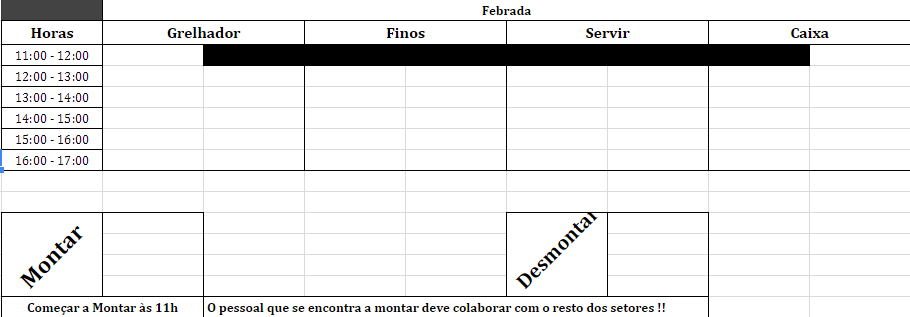
\includegraphics[width=0.88\textwidth]{imagens/escalas.png}
        \item Ligar a máquina de finos à corrente pelo menos um dia antes da febrada, para garantir que esta refresca.
        \item Pedir trocos ao Tesoureiro o quanto antes, para ter caixa inicial.
        \item Senhas e preçário: é essencial fazer senhas para cada evento específico, imprimi-las e cortá-las, bem como imprimir o preçário, que é discutido primeiro com o Tesoureiro. Não se esqueçam de rasgar e deitar as senhas ao lixo assim que as recebam durante a febrada para impedir as habituais borlas.
    \end{itemize}

    \item O dia da febrada
    \begin{itemize}
        \item Se forem seguidos todos os passos acima terão uma febrada de sucesso e neste dia só precisam de ir buscar as febras e o pão entretanto encomendados, montar a tenda e temperar as febras.
        \item Tempero das febras: juntem toda a carne num alguidar e deitem bastante massa de alho, pimentão doce, ervas de Provence, pimenta branca, sal e por fim, um fino. Usem luvas!
        \item É importante terem febras prontas antes da hora de afluência (meio-dia quando as mesmas são à hora de almoço), de modo a que não existam filas à hora de almoço e tudo flua super-rápido.
        \item No fim, deixem tudo limpo e arrumado e se ainda houver cerveja no barril, façam bar aberto a troco de um preço reduzido, as pessoas gostam e de outra maneira a cerveja iria para o lixo. O mesmo se aplica à carne e ao pão. Tentem sempre não desperdiçar.
        \item Caso sobre pão, contactem uma instituição de recolha de comida, que fará a recolha de imediato.
    \end{itemize}
\end{itemize}
}
{ % FALSE
}

% ========================
% # Coffee-Breaks        #
% ========================

\subsubsection{Coffee-Breaks}

O Pelouro da Administração tem uma forte ligação com todos os outros estando presente, nomeadamente, quando existem coffee-breaks nas atividades. Estes constituem uma benesse de reduzido custo e fácil organização sendo muito utilizados nos workshops do Pelouro das Saídas Profissionais e Formação. Para os organizar há que ter, no entanto, alguns cuidados para que os mesmos corram da melhor forma possível.
É então necessário fazer os seguintes passos:
\begin{enumerate}
    \item Comunicar com o responsável da atividade, de modo a saber: horas, local e número de participantes esperado.
    \item Combinar se é necessário ou não ajuda logística para a realização dos Coffee-Breaks ou se é apenas necessário deixar todo o material pronto a levar na sala do Núcleo.
\end{enumerate}

Material sempre necessário:
\begin{itemize}
    \item Pratos e copos descartáveis;
    \item Guardanapos;
    \item Várias garrafas de água para os oradores do evento.
\end{itemize}

Quanto à comida basta fazer uma estimativa a olho, tendo em conta o número de participantes colocando-se, habitualmente, bolachas, biscoitos, águas e sumos. Caso haja disponibilidade financeira pode-se aproveitar as várias máquinas de café existentes para servir café e servir alguns doces, vindo de pastelarias, e frutas. Com o \acrshort{ene3} e o Bot Olympics, este ano, tivemos uma boa injeção de alimentos da Dancake, pelo que não foi necessário comprar nada ao longo do ano, exceto as garrafas de água. Contudo, ficou em falta o serviço de café e fruta.

Um ponto importante, relacionado com o desperdício, é que as sobras são expostas no Núcleo, com um aviso a dizer que se podem comer, desaparecendo tudo em menos de 24h.

% ========================
% # Inventário           #
% ========================

\subsubsection{Inventário e Empréstimos}

A criação do inventário foi uma ideia que surgiu desde o início do mandato desde o momento em que se verificou que era impossível saber todo o material do qual o \acrshort{neeec} era proprietário e o material do qual a \acrshort{fctuc} era proprietária mas que estava alocado ao \acrshort{neeec}. Adicionalmente, no início do mandato várias foram as pessoas a vir à Sala do Núcleo solicitar materiais que alegavam ser seus, não havendo registo de nada. Este foi um processo que demorou quase a totalidade do mandato para ser finalizado.

Inicialmente numa fase embrionária, onde todo o material foi registado num Excel que possuia um separador extra para os materiais que eram emprestados. Como tal, foi necessário etiquetar tudo o que pertencia ao Núcleo, atribuindo um código único a cada produto. Para isso, foi feito um pedido ao GRI, que nos forneceu etiquetas impressas com o símbolo do \acrshort{neeec} e com um código numérico e de barras, diferente de cada um.

Adicionalmente foi criado um novo modelo de declaração de empréstimos onde eram solicitadas várias informações dos requerentes bem inseridos os dados do material emprestado, garantindo assim que eram declarados os valores de caução recebidos pelo \acrshort{neeec} e os valores restituídos após a devolução do material. Ao se usar este método para registar os empréstimos, passou a ser muito mais fácil controlar todas as entradas e saídas de materiais do Núcleo. Contudo, o facto de ser um modelo de preenchimento manual, associado ao facto de muitos empréstimos terem de ser processados à pressa, levou a que houvesse vários erros no preenchimento dos documentos que poderiam ter causado alguns problemas como, por exemplo, a devolução repetida da caução algo que, felizmente, nunca ocorreu.

No 2º semestre, com a introdução da plataforma informática de gestão interna, esse Excel deixou de existir, passando-se a registar todos os materiais nessa mesma plataforma. Como tal, foi necessário rever todo o inventário, antes de chegar à sua forma final. Nesta revisão, as etiquetas foram todas substituídas para se poder colocar um código QR Code em vez de um código barras, código esse que é lido pela plataforma através de uma câmara. Também os empréstimos passaram a ser processados pela plataforma sendo os documentos preenchidos de forma automática, bastando imprimi-los e assiná-los. Por implementar, fica a separação dos documentos de empréstimos em dois: um modelo para preencher quando o empréstimo é feito e outro para quando o empréstimo é devolvido, algo essencial para a finalização bem sucedida deste processo.

\ifthenelse{\boolean{empresas}}
{ %TRUE
}
{ % FALSE
Todo o inventário do \acrshort{neeec}, no final deste mandato, pode ser consultado em \ref{inventario}.
}
No sistema de gestão informática, cada produto tem várias características associadas: 
\begin{itemize}
\item SKU ID - código de identificação único, diferente para cada produto;
\item Nome do Material - o preenchimento deste campo deve ser feito com cuidado para que o inventário se mantenha atualizado de forma fácil: por exemplo, colocar "armário cinzento do canto" faz com que o inventário fique desatualizado sempre que o armário referido for mudado de sítio sem que seja atualizado o inventário pelo que é preferível colocar "armário cinzento de meia altura";
\item Se é emprestável ou não - este campo serve para indicar se os materiais podem ser emprestados (por exemplo, uma tenda é emprestável mas um armário não);
\item Valor da caução - este valor só deve ser preenchido se o material for emprestável e é automaticamente inserido no ato de empréstimos;
\item Local onde está armazenado - esta informação é muito importante uma vez que o \acrshort{neeec}, cada vez mais, detém mais locais para além da Sala do Núcleo;
\item Código da \acrshort{fctuc} - esta variável serve para inserir o código dos produtos caso eles sejam da \acrshort{fctuc}. Assim é possível interligar o nosso sistema com o do Aprovisionamento do \acrshort{deec};
\item Se está ou não emprestado
\end{itemize}

Deste modo, sempre que for necessário fazer um empréstimo basta aceder à plataforma do interno, adicionar as informações da pessoa/entidade à base de dados e, posteriormente, selecionar o material a ser emprestado. Depois disso é gerado um documento, com todas as informações relativas a esse empréstimo, inclusive a caução total. Imprime-se em duplicado e ambas as entidades assinam. Recebe-se a caução e esta só é devolvida na totalidade se o material estiver nas mesmas condições em que estava antes do empréstimo.

\clearpage
% ========================
% # Cultura e Lazer      #
% ========================

\section{Cultura e Lazer}

\subsection{Introdução}

No presente ano letivo, a equipa deste Pelouro foi inicialmente constituída por sete elementos contudo, após algumas mudanças terminou o ano letivo com, tecnicamente, cinco elementos e um CG diferente. Para todas as atividades tentou-se dividir as tarefas pelas várias pessoas (uma pessoa ficava encarregue por uma tarefa, e assim sucessivamente) dando inicialmente a opção de escolha a cada e nas semanas/dias que antecipavam o evento tentava-se realizar pequenas reuniões com todos os elementos para saber o “ponto de situação”, dar sugestões, etc. Esta divisão de tarefas foi, no geral, uma decisão que não trouxe grandes problema e sempre que trouxe estes tentavam ser resolvidos de forma rápida, para que não causassem grandes complicações no evento e, caso sucedesse, pudessem ser colmatadas com os restantes elementos.

\subsection{Atividades}

% ========================
% # Visita à Alta        #
% ========================

\subsubsection{Visita à Alta }

A visita à alta realizou-se no dia 27 de setembro com o objetivo de integrar a praxe com uma visita organizada pelo \acrshort{neeec} à parte histórica da cidade de Coimbra.

Existiu, no início, um contratempo no percurso predefinido pela equipa do \acrshort{neeec}. Como apenas existia uma pessoa referente a essa equipa a acompanhar a praxe, e não estava 100\% integrada com o programa da atividade, foi influenciado pelo grupo de Doutores que acompanhavam os caloiros o que provocou um desvio no percurso e atrasos na Visita ao Pátio das Escolas.

Este evento é uma oportunidade de mostrar aos caloiros um pouco da cidade de Coimbra, nomeadamente a zona circundante da \acrlong{uc}. Enquadrado numa situação de praxe académica funciona melhor pois ajuda no transporte e guia dos caloiros. Há que tentar que comece cedo de forma a que os alunos possam visitar todos os locais.
Sugestões para futuras realizações:
\begin{itemize}
\item Contactar antecipadamente a Biblioteca Geral para confirmar o número de pessoas;
\item Chegando à porta férrea dividir os alunos por grupos de forma a facilitar as visitas;
\item Tentar fazer \textit{guide lines} com informações sobre os locais a visitar;
\item Ter mais do que um fotógrafo;
\item Criar um género de Peddy Paper ao invés de uma visita ao grupo permitindo que as visitas sejam feitas em grupos mais pequenos;
\item Aproveitar o verão para organizar melhor o evento.
\end{itemize}

% ========================
% # Visita à AAC         #
% ========================

\subsubsection{Visita à AAC}

A Visita à \acrshort{aac} foi uma visita guiada às instalações da \acrshort{aac}, na Rua Padre António Vieira, nomeadamente às suas Secções Culturais e Desportivas para alunos do primeiro ano, orientada por membros das Relações Externas da \acrshort{aac}. Foi um evento que contou com poucos participantes (vinte e sete), o que se deve ao facto de não ter ocorrido praxe académica que levasse os alunos até ao evento, por motivos que nos são alheios mas que, em edições futuras, devem ser mais cuidados. Os alunos que participaram consideraram a atividade um pouco aborrecida pois apenas algumas secções eram “interessantes”.
Este evento tem muito mais sentido se realizado de forma integrada na praxe de forma a abranger mais alunos, divididos em grupos.


% ================================
% # \acrshort{uc} Plantas        #
% ================================

\subsubsection{UC Plantas}

Organizado pela \acrshort{uc}, este evento era destinado aos alunos do primeiro ano e contou com uma pequena visita ao Jardim Botânico da \acrshort{uc} e a possibilidade de adotar uma planta. No futuro era possível os alunos entregarem de novo a planta para que esta pudesse ser plantada no Jardim. Ao contrário da Visita à \acrshort{aac}, o número de participantes foi elevado (devido à realização de praxe) mas foram poucos os participantes (quatro) que decidiram adotar a planta, demonstrando uma clara falta de interesse no evento.

Apesar de interessante a proposta do evento, não houve grande adesão, muito pelo facto de os alunos não terem vontade de andar com uma planta nas mãos o resto do dia e depois cuidar e tratar dela.


% ================================
% # Magusto                      #
% ================================

\subsubsection{Magusto}

Este evento já decorre de forma tradicional todos os anos, permitindo o convívio entre alunos, professores e funcionários do \acrshort{deec}, onde são distribuídas castanhas e jeropiga. Para além disso contou-se com a realização de torneio de sueca e matraquilhos, a decorrer em simultâneo, da responsabilidade do Pelouro de Desporto.
\ifthenelse{\boolean{biblia}}
{ % TRUE
Este é um evento que, por ser gratuito e divertido, atrai bastantes participantes.
A mudança de dia do evento (quinta feira, em vez de quarta como era habitual) fez com que a sua adesão fosse ainda mais elevada, mas prejudicou os torneios devido à ocorrência em simultâneo de aulas e frequências.
}
{ % FALSE
}

Há que ter em atenção a forma como são assadas castanhas: como não são assadas pelo Núcleo, mas sim por pela Padaria de São João convém definir um prazo um bocado mais cedo para assar de forma a ter as castanhas prontas a servir à hora de início do evento. Outro aspeto a ter em consideração é como se obtém as castanhas: caso haja possibilidade de obter gratuitamente, apanhando, é de aproveitar, ao invés de se gastar dinheiro a comprar. Há que ter muita atenção à limpeza do espaço: o evento tem sido realizado na esplanada do bar pelo que é de maior importância que no final do evento esteja tudo limpo, nomeadamente que sejam varridas as cascas de castanhas, algo que é difícil por anoitecer cedo.


% ================================
% # Quiz                         #
% ================================

\subsubsection{Quiz Cultural}

O quiz cultural foi um evento realizado aquando do Mês Solidário, onde equipas de dois elementos competiram ao responder a perguntas de vários temas (Cinema/Séries, Música, Geografia e Cultura Geral). As equipas responderam (numa “placa” de resposta fornecida) às perguntas apresentadas (através de um PowerPoint) e receberam/perderam pontos de acordo com as suas respostas. No final da competição, a equipa com maior pontuação foi a vencedora.

A placa de resposta foi feita por um elemento do Pelouro e era constituída por uma pequena placa de cartão e papel cavalinho, forrada a papel autocolante, onde os participantes podiam escrever com marcadores as suas respostas, mostrar as mesmas e, por fim, apagar com um papel e assim sucessivamente.

O evento realizou-se no auditório A.5.2 do \acrshort{deec} que, tendo em conta o número de participantes (no presente ano letivo, contou-se com dez participantes), foi um bom local pois conseguiu-se colocar todas as equipas e ainda espaçá-las. Caso o número de participantes fosse superior, este evento decorreria melhor numa sala (por exemplo a T.4.1 ou T.4.4 do \acrshort{deec}) ou até mesmo num dos auditórios de maiores dimensões. 

O feedback dos participantes foi extremamente positivo: gostaram da atividade e divertiram-se. Para muitos, a hora de realização do evento (quarta-feira às 18h) foi um problema pelo que esta deveria ter ocorrido mais cedo.

É necessário ter em atenção algumas situações: rever muito bem as perguntas e respostas para que não haja problemas com respostas erradas. Usar uma tabela de pontuações mais “automática” para que quem esteja a apontar as mesmas não perca muito tempo a confirmar os pontos a atribuir ou retirar às equipas (exemplo: em vez de apontar o número de pontos que a equipa obteve numa pergunta, colocar apenas um A (acertou) ou um E (errou) e definir os seus valores no excel).

Este é um evento que costuma ter pouca adesão mas que costuma ser muito divertido para quem participa pelo que a sua realização nos parece importante mas deve ser feita uma aposta maior na sua divulgação.


% ================================
% # Noite de Fados               #
% ================================

\subsubsection{Noite de Fados}

Realizado em conjunto com o \acrshort{nei}, este evento contou com uma febrada e atuações de uma tuna (Quantunna) e de um grupo de fados (Capas ao Luar) oferecendo assim uma noite diferente aos estudantes de ambos os departamentos: (\acrshort{deec} e \acrshort{dei}).

Sendo este um evento organizado com um outro Núcleo por vezes torna-se difícil a comunicação entre ambos. Foi feita uma divisão de tarefas por núcleos, o foi uma boa ideia, mas devido a diferentes formas de trabalho certos aspetos do evento deixaram muito a desejar (por exemplo, a divulgação do evento, particularmente no nosso Departamento, pois os cartazes – apesar da constante insistência - foram feitos, entregues e divulgados pelo \acrshort{nei} demasiado perto do evento, sem que o \acrshort{neeec} pudesse dar a sua opinião relativamente à imagem e eventuais erros, o que se traduziu numa maior adesão por parte dos alunos do \acrshort{dei}). A escala de trabalhos deve ser divulgada com alguma antecedência para que não haja problemas de preenchimento.

Para além da febrada e das atuações, colocou-se a mesa de matraquilhos do \acrshort{neeec} para quem quisesse jogar, exceto durante as atuações das tunas e grupos de fado, devido ao barulho. Os jogos foram gratuitos durante toda a noite o que atraiu muita gente. Esta situação é um pouco “sensível” pois, caso os matraquilhos fossem pagos (como normalmente são) sempre era uma fonte de rendimento para o Núcleo, mas, por outro lado, corre-se o risco de, caso seja pago, o número de interessados não ser tão grande eliminando, então, essa fonte de rendimento. Consideramos que isto é algo que se deva manter, principalmente gratuitamente, ou até mesmo criar uma pequena competição/torneio (com por exemplo, febras e/ou finos como prémio) pois é algo que atrai pessoal. De reforçar que, caso se mantenham os matraquilhos, estes devem estar bloqueados durante as atuações.

Apesar de todos os problemas já referidos, o evento correu bem e permitiu oferecer aos alunos de ambos os departamentos uma noite diferente.


% ================================
% # Semana Cultural e Desportiva #
% ================================

\subsubsection{Semana Cultural e Desportiva}

Pela primeira vez, foi realizada um Semana Desportiva e Cultural (“NEEEC Sports \& Culture Week”) organizada em parceria com o Pelouro do Desporto. Durante esta semana (segunda, terça, quarta e quinta) foram propostas diversas atividades aos alunos do \acrshort{deec}, tanto de cariz desportivo como de cariz mais cultural/lúdico.

No primeiro dia, realizou-se uma pequena feira composta pelas diversas secções culturais e desportivas da \acrshort{aac} para demonstrar a oferta e o que nelas se faz. Após várias tentativas de comunicação com todas as secções culturais só se obteve resposta de duas (Grupo Ecológico e SOS Estudante) e apenas uma, Grupo Ecológico, esteve presente.

No segundo dia, do final da manhã até meio da tarde, contou-se com a presença do Simology, um simulador realista de condução. O simulador foi colocado na sala de convívio e requeria uma inscrição prévia com um custo de 2€. Devido ao desconhecimento do que era o Simology, as inscrições até ao dia foram muito poucas (cerca de cinco). Uma vez montado, os alunos demonstraram bastante interesse na atividade e muitos inscreveram-se na hora de participar fazendo com que se tivesse de prolongar por mais uma hora o aluguer do material, continuando a haver fila na hora de fecho. Foi uma atividade um bocado dispendiosa e que trouxe um pouco de prejuízo mas foi sem dúvida a atividade, por parte do Pelouro da Cultura, que mais curiosidade e participação teve por parte dos alunos, ao longo de todo o ano. Os inscritos tiveram a oportunidade de experimentar o simulador (com recurso a óculos de realidade virtual) e no final era apontado o tempo que os participantes demoravam a percorrer a pista. O inscrito com melhor tempo (i.e. com o menor tempo) teve direito a um prémio.

De tarde, realizou-se um torneio de FIFA 18. Com inscrição prévia, os participantes competiam entre si de forma aleatória numa série de jogos para descobrir quem seria o vencedor (o torneio foi “gerido” através do site https://challonge.com/). Estava também proposto um torneio de Street Fighter IV que acabou por não se realizar por falta de inscrições para o mesmo.

No terceiro dia, realizou-se uma tarde de jogos de tabuleiro, de participação gratuita. Feita na sala de convívio, os alunos tinham à sua disponibilização diversos jogos de tabuleiro (Monopólio, Party \& Co., Trivial Pursuit, Mikado, Uno, Damas, Xadrez, entre outros) que podiam usufruir. O tempo de duração do evento foi diminuído (inicialmente duas horas, passou para uma hora) porque não houve participantes.

No quarto dia propôs-se a realização de um novo Quiz, à semelhança do anterior. O evento não foi realizado devido à falta de inscrições suficientes (apenas uma equipa se inscreveu).

No geral, sendo um evento novo os alunos não demonstraram grande interesse, o que se traduziu em muito poucas inscrições nos eventos. Apesar disso, consideramos ser um evento bastante interessante e com grande potencial no futuro, se mais divulgado e colocado numa data melhor. Os torneios de videojogos convém serem de jogos que os participantes conheçam e tenham interesse (algo que se verificou ao haver inscrições no torneio de FIFA e não no torneio de Street Fighter). Os jogos de tabuleiro não parecem ter grande interesse por parte dos alunos (algo que é comprovado durante o resto do ano, onde os alunos nos seus tempos livres não requisitam alguns dos jogos oferecidos pelo \acrshort{neeec} (Damas, Xadrez, Cartas, etc.) mas requisitam bastante as raquetes de ténis de mesa, por exemplo).


% ================================
% # Peddy Tascas                 #
% ================================

\subsubsection{Peddy Tascas} \label{subsubsec:atividades-cultura-peddy}

Este evento é realizado, habitualmente, pela altura das Festas Académicas (Festa das Latas e Imposição de Insígnias e Queima das Fitas), mas no presente ano letivo, dado a falta de adesão em anos anteriores, realizou-se apenas uma edição, nas semanas antes da Queima das Fitas. Neste evento os participantes, organizados em equipas de quatro a cinco elementos, visitam diversas tascas e “pontos \acrshort{neeec}” onde têm uma bebida que têm de consumir, ganhando assim pontos. Nesta edição, os prémios foram bilhetes gerais e pontuais para a Queima das Fitas, o que atraiu mais pessoas ao evento. Durante o percurso foram colocados alguns “Pontos \acrshort{neeec}”. Estes consistiam em locais onde membros do Núcleo serviam uma bebida aos membros das equipas (uma bebida diferente por ponto) e faziam pequenos desafios onde as equipas, caso bem sucedidas a completar os desafios, poderiam ganhar mais pontos.

É um evento de maior escala e como tal a ajuda, não só da equipa do Pelouro, mas também de todos os membros do Núcleo é essencial (são necessários acompanhantes para as equipas, pessoas para estarem nos “Pontos \acrshort{neeec}”, entre outros). É também muito importante prever algumas situações para que não haja problemas, como por exemplo, garantir que nos “Pontos \acrshort{neeec}” não acaba bebida (comprar sempre a mais do que o previsto). Caso sobre bebida de algum “Ponto \acrshort{neeec}”, esta pode ser sempre utilizada no ponto de chegada de forma a dar a possibilidade dos participantes obterem mais pontos.

O pagamento das tascas deve ser efetuado perto do fim do evento, tendo em atenção os horários de funcionamento das mesmas.

Deixamos agora algumas sugestões para futuras realizações:
\begin{itemize}
    \item Tal como referido anteriormente há que garantir que não há falta de material, nomeadamente bebidas, copos, etc;
    \item Distribuir pelas tascas, antes do evento começar, uma folha de presenças com as equipas de forma a garantir que, caso seja feito o pagamento da tasca antes de uma ou mais equipas terem passado pela mesma, não lhes seja recusada bebida, algo que acontece frequentemente; 
    \item Ter em atenção a todos os pedidos impostos pelas tascas e caso não seja dito nada, perguntar e garantir que não surgem imprevistos (horas de encerramento, algumas tascas começam a servir refeições a partir de certa hora e as equipas têm de passar todas por lá antes da hora imposta, etc.);
    \item Ter em atenção aos acompanhantes das equipas. É impossível garantir que não bebam, mas ter em atenção que, obviamente, não podem beber da mesma forma que os participantes para que não haja problemas de qualquer natureza (seja no preenchimento de tabelas de pontuação, seja problemas com as pessoas, e assim);
    \item Caso haja atividades a serem realizadas, ter o material sempre preparado e em boas condições;
    \item Ter preparado mais do que dois percursos (ou então ter em conta o número de equipas inscritas) de forma a garantir, ou pelo menos prevenir, que uma ou mais equipas se cruze com outra podendo atrasar ou criar mau ambiente de funcionamento na tasca;
    \item Criar uma forma de serem as tascas a registar os pontos para evitar que haja equipas a ser favorecidas pelo elemento que as acompanha, ainda para mais quando há prémios tão aliciantes, como houve este ano.
\end{itemize}

Apesar do trabalho e eventuais problemas que possam surgir, este é um evento que atrai muitos participantes (principalmente pela proximidade com os eventos da Queima das Fitas ou Latada) e que todos gostam de participar.

% ================================
% # Omen                         #
% ================================

\subsubsection{HP by Omen University Challenge}

Este evento é, habitualmente, realizado nos finais de maio. Consiste numa competição, de inscrição gratuita, de FIFA onde os vencedores podem ganhar vales de compras entre 25€ e 100€ e acesso à final da competição, realizada em Lisboa. Este evento é independente do \acrshort{neeec} sendo organizado pela E2Tech e, portanto, toda a logística do evento é assegurada pela mesma. O \acrshort{neeec} apenas fica encarregue de retirar tudo o que se encontra na sala de convívio (ou do local escolhido para o realizar) e abrir as portas para os funcionários da empresa transportarem e montarem o material de manhã, pelas 8h.

Deixamos algumas sugestões para futuras realizações:
\begin{itemize}
\item No presente ano de 2017-2018, foi pedido ao \acrshort{neeec}, pelos organizadores, uma lista com alguns nomes só para “encher inscrições”, uma vez que uma das empresas envolvidas exige números mínimos. Caso tal seja voltado a pedir, deve-se ter em atenção aos nomes colocados pois, ao contrário do que foi dito pela organização, os nomes são chamados em “voz alta” para assinalar a presença dos participantes, podendo criar alguns problemas caso haja nomes de pessoas que não se inscreveram e se encontrem presentes na sala, como ocorreu;
\item Tal como dito anteriormente, o evento é totalmente gratuito e isto é algo que se deve considerar manter pois cobrar inscrição pode fazer com que muitos participantes acabem por não se inscrever (até porque existem alguns participantes que não são alunos do \acrshort{deec}, vindo de fora apenas para competir);
\item Apesar de, nos últimos anos, o evento se ter realizado em maio, a data pode ser repensada uma vez que as eliminatórias começam em fevereiro. Para tal, basta contactar a empresa dinamizadora no início do ano letivo para se estabelecer uma nova data e assim trazer mais participantes para o evento;
\item É importante manter alguma atividade a decorrer em paralelo com o evento de forma a atrair pessoas para o mesmo ou escolher uma data em que o Departamento esteja cheio. No ano passado, a data escolhida foi 24 de maio, uma quarta-feira, última de aulas, em que o Departamento estava vazio mas a realização de uma febrada dos Carros da Queima das Fitas do ano seguinte nos Jardins do NEEEC fez com que o evento estivesse sempre movimento. Este ano a data escolhida foi semelhante, 23 de maio, última quarta-feira de aulas do semestre, estando novamente o Departamento vazio mas, como desta vez não existia nenhuma atividade a decorrer em simultâneo, o evento teve vários momentos, na altura de uso livre, em que estava vazio.
\end{itemize}

\clearpage
% ========================
% # Desporto             #
% ========================

\section{Desporto}

No presente ano letivo, a equipa do Pelouro do Desporto foi constituída por 8 elementos. Após a realização de várias atividades onde o Coordenador Geral do Pelouro, André Soares, não se apresentou como responsável pelo Pelouro, a Direção do \acrshort{neeec} decidiu demiti-lo e tomou a gestão do Pelouro, provisoriamente, até à conclusão da realização da final da Liga \acrshort{deec}. Assim, o Pedro Henriques foi convidado a assumir as funções de Coordenador Geral tendo, no entanto, deparado-se com um plano de atividades por realizar que não tinha sido feito por si. Este Pelouro acabou, no entanto, por ser bastante ativo tendo-se realizado várias atividades novas nomeadamente uma semana desportiva e cultural, um passeio de bicicleta e a descida do rio. Por fazer, ficou a visita ao estádio cidade de Coimbra e à Academia Briosa XXI bem como a organização de uma ida a um jogo da Académica/OAF. No que toca à organização interna, o Pelouro esteve sempre bastante dependente do CG bem como da Direção mas todos os membros do Pelouro estiveram sempre disponíveis a ajudar em tudo, contudo, verificou-se que o número elevado de membros neste Pelouro (8) acabou por dificultar mais o trabalho do mesmo do que facilitar.

\subsection{Atividades}

% ====================================
% # Transmissão dos Jogos da Seleção #
% ====================================

\subsubsection{Transmissão dos Jogos da Seleção}

No mês de junho foram transmitidos os jogos da seleção nacional de futebol, para a Taça das Confederações, Portugal vs Rússia (2ª jornada da fase de grupos) e Portugal vs Chile (meias finais). O jogo da 1ª e 3ª jornadas não foram transmitidos uma vez que pelas suas horas e/ou dias da semana em que calhavam não havia público suficiente no DEEC para se justificar a realização da atividade.

O local escolhido para o evento foi a sala de convívio, mudando-se a disposição da sala completamente: pôs-se filas de cadeiras ao longo de toda a sala com um projetor apontado para a parede da reprografia. Tiveram de se por panos escuros nas janelas mais próximas do projetor, uma vez que as cortinas deixavam passar muita luz, impedindo a possibilidade de se ver a transmissão decentemente.

Para criar uma dinâmica gira durante o jogo fez-se uma cachorrada onde se venderam minis frescas, cachorros e águas, sendo que a zona de trabalho era junto à parede do Núcleo, atrás da transmissão.

\ifthenelse{\boolean{biblia}}
{ % TRUE
Em termos logísticos foi bastante fácil organizar o evento tendo sido a parte mais trabalhosa a cachorrada pois requer que haja pessoas sempre disponíveis para servir as pessoas, ou seja uma escala, o que é sempre complicado numa época de exames.
}
{ % FALSE
}

O evento teve imensa adesão, tendo em conta que estávamos em plena época de exames e o Departamento não tinha muita gente. Ao longo do evento, dada a falta de cadeiras que havia na sala de convívio (situação entretanto resolvida com as cadeiras de jardim) foi necessário ir buscar várias cadeiras às salas de aula da torre T.

% ================================
% # Caloiros VS Doutores         #
% ================================

\subsubsection{Caloiros VS Doutores}

No âmbito da receção ao caloiro, o Pelouro do Desporto decidiu fazer um jogo de futsal 7 x 7 de Caloiros vs Doutores. Este evento é já muito habitual noutros núcleos pelo que achámos por bem trazê-lo para o nosso Núcleo.

O evento realizou-se numa quarta-feira à noite, após uma praxe, no mesmo dia da visita à alta. De realçar que, devido à praxe, existiu uma claque no evento o que dinamizou muito o mesmo. É também de realçar que a praxe não esteve muito disponível para manter as atividades praxísticas desde o final da visita à alta até ao início do jogo o que provocou uma claque mais reduzida, não deixando, no entanto, de ser muito divertida. No futuro, aconselhamos a uma maior coordenação das atividades com a praxe.

O jogo de futsal 7 x 7 teve um limite de 14 jogadores por equipa e duas partes com a duração de 30 minutos, cada. O campo escolhido foi o campo de Santa Cruz tendo o aluguer do mesmo um custo de 42 euros. A inscrição teve um custo de 2 euros por pessoa para cobrir a despesa do campo. De realçar que as inscrições não esgotaram, mas ficaram muito perto disso (13 inscritos em cada equipa).

No futuro é necessária uma maior organização interna do Pelouro para a atividade, principalmente no que diz respeito ao cumprimento da escala (que para este evento foi muito simples) e à verificação de pagamentos (os problemas que ocorreram, não voltariam a ocorrer com as modificações entretanto feitas no que toca à gestão de inscrições entretanto feitas no \acrshort{neeec}). Destacamos que o evento é muito divertido, agradou a todos os participantes, mas que só tem piada se for feito com a praxe. Foi também uma ideia nossa, mas que acabou por não avançar por não ter viabilidade financeira nem logística, realizar um pequeno convívio com finos junto ao jogo, algo que se for mais bem pensado poderá ser feito no futuro.


% ===================================
% # Torneio de Sueca e Matraquilhos #
% ===================================

\subsubsection{Torneio de Sueca e Matraquilhos}

Com a realização do tradicional magusto, responsabilidade do Pelouro da Cultura e Lazer, é habitual fazer-se um torneio de sueca. Este ano, decidimos também fazer um torneio de matraquilhos. Para tal, foi feito e divulgado um regulamento para cada torneio, essenciais para o bom funcionamento do mesmo, e foram anunciados prémios, que consistiam em finos, para os vencedores.

O evento acabou por ter vários problemas uma vez que este se realizou a uma quinta-feira, havendo aulas e frequências em simultâneo, o que dificultou a presença de participantes e pessoas para trabalhar na atividade. Por sua vez, o CG do Pelouro decidiu atrasar em duas horas o início do torneio para tentar ter mais inscritos. Assim, quem podia à hora marcada deixou de poder e quem não podia não soube da alteração pelo que também não participou. Ambos os torneios acabaram por se realizar com poucas equipas (cerca de 3) tendo o mesmo prolongado-se até muito tarde, muito para além da hora prevista para o fim da escala, fazendo com que membros do Pelouro tivessem de se revezar entre si para conseguir terminar o evento. Por sua vez, o CG, meia hora após o início dos torneios, decidiu ir para Viseu sem avisar ninguém, tendo deixado dois membros do Pelouro encarregue dos dois eventos, tendo sido, portanto, demitido no dia seguinte. Um dos membros do Pelouro era também participante do torneio que estava a vigiar o que dificultou, ainda mais, a situação.

Uma vez que o magusto é feito nos jardins do bar e anoitece cedo em novembro, teve ainda de se arranjar soluções, à pressa, para mudar de local quando anoiteceu. Ambos os torneios, apesar de terem poucos participantes, terminaram numa altura em que já quase ninguém estava no departamento, havendo inclusive desclassificações porque equipas precisavam de se ir embora. Em suma, este foi um evento super desorganizado que, obviamente, deve ter continuidade mas deve ser organizado de forma muito mais ponderada.

% ================================
% # Liga DEEC                    #
% ================================

\subsubsection{Liga DEEC}

Como é tradicional, realizou-se um torneio de futsal que dá acesso à Liga Polo 2. A este torneio optámos por chamar Liga \acrshort{deec} e não Liga Polo 2 uma vez que o evento é exclusivamente organizado pelo \acrshort{neeec} e não tem sequer as mesmas regras da Liga Polo 2 (de notar, que só o NEEC e o NEEA é que denominam as suas eliminatórias como Liga Polo 2). Este evento realizou-se como costume, em novembro, tendo coincidido com um período muito conturbado do Pelouro pelo que foi organizado pela Direção em conjunto com o Pelouro e executado pelo Pelouro.

Decidiu-se delimitar de imediato o número de equipas a 8 e permitir um número de elementos entre 6 e 8 em cada equipa. Fez-se também um regulamento completamente novo e detalhadamente pensado em reunião de Pelouro, o qual foi muito positivo para a execução do torneio. Recomendamos a restrição do número de equipas logo de início pois tal permite delinear o torneio à partida no regulamento e na organização do mesmo. Pelo mesmo motivo, recomendamos, no futuro, a que se limite o número de elementos das equipas não permitindo equipas de tamanhos diferentes, o que trouxe problemas (embora simples).

As inscrições tinham um custo de 5€ por pessoa e o preço foi anunciado como preço individual e não de equipa para não assustar as pessoas. Quanto à logística das inscrições, as mesmas esgotaram e houve equipas inscritas a mais. Foi cumprido o regulamento e dada primazia a quem exerceu o pagamento em primeiro lugar o que, por se tratar de um fim de semana, deu privilégio a quem pagou por transferência, provocando amuos nas equipas excluídas (foi excluída uma equipa e outra desistiu). De realçar, no entanto, que as inscrições demoraram ainda alguns dias para começar tendo sido fechadas apenas no sábado antes do evento.

Para a logística do torneio, preparou-se um excel que ordenava automaticamente as equipas pelos grupos (fazia o sorteio) e dava para depois inserir os detalhes de cada jogo. Este excel facilitou imenso o trabalho durante o torneio e o mesmo encontra-se disponível para ser usado em futuras edições e adaptado a outras modalidades. Existiu também uma ficha de jogo que, precisa de várias melhorias no futuro (nomeadamente: não há cantos no futsal, o ponto dos jogadores que não compareceram ou que chegaram atrasados deve estar na mesma tabela de amarelos e vermelhos para que seja de fácil preenchimento e dois espaços para árbitros de mesa).

Em relação ao evento em si:
\begin{itemize}
\item Foi criada uma escala que contemplava apanha-bolas, ajuda logística além dos árbitros o que possibilitou dar uma qualidade muito grande ao evento. O apanha-bola bola é uma pessoa essencial e deve estar sempre escalado.
\item Venda de panikes, sumos e águas: a partir da segunda noite, uma vez que na primeira noite muitas pessoas foram comprar estes elementos a outros lados, passou a estar disponível para venda alguns produtos alimentares o que permitiu ganhar algum dinheiro para compensar as elevadas despesas do evento.
\item Música: nos intervalos e no início e fim da noite havia sempre música o que animava muito o evento.
\item Início de cada noite: o início de cada noite tinha sempre atrasos (após o primeiro dia, o atraso era maior na organização no que nas equipas) o que fez com que ficássemos todas as noites após a hora final (23h30). A partir da meia noite, o segurança queria-se ir embora não se importando de esperar no primeiro dia, mas ficando visivelmente chateado nos restantes com destaque na final que ameaçou os presentes de os fechar dentro da escola uma vez que a hora já excedia demais.
\item Os jogos tiveram durações maiores nas meias finais e nas finais o que provocou um atraso muito grande nesse dia, apesar de se realizarem 4 jogos e não 6 como nos outros dias.
\item Foi criada pelos membros do Pelouro uma faixa da Liga \acrshort{deec} o que foi engraçado para as fotos e não acarretou custos uma vez que foi feito de forma manual, contudo, com a chuva teve de ir para o lixo.
\item Final: a final foi transmitida em direto, teve música dos campeões e a entrega de medalhas foi feita em estilo pódio utilizando, para isso, as escadas existentes junto ao campo. Não existiu troféu, mas foi entregue a grade de cerveja o que permitiu uma festa muito engraçada dos vencedores.
\end{itemize}


% ================================
% # \acrshort{neeec} VS Profs               #
% ================================

\subsubsection{NEEEC VS Profs}

O \acrshort{neeec} vs PROFS é um jogo de futebol de salão, 5x5, pertencente ao mês solidário, onde os elementos do \acrshort{neeec} defrontam os professores do \acrshort{deec} num espírito de convívio tendo a atividade uma inscrição simbólica de um bem alimentar. Este evento é restrito aos elementos do \acrshort{neeec} pois caso contrário traria um défice ainda maior de alunos perante professores.

O convite aos professores este ano foi alargado aos funcionários sendo que o Eng. Maia e o Tito manifestaram bastante interesse em ir mas não puderam, por motivos pessoais. É muito importante partilhar bem este evento junto dos professores e garantir que os emails são entregues. Como em tudo, o melhor é fazer o convite pessoalmente, garantindo assim mais entradas. Alguns professores como o professor Peixoto, o professor Marco e o professor Crisóstomo costumam marcar sempre presença.

Este ano, o jogo decorreu no campo da Escola Secundária Infanta D. Maria, no mesmo local da Liga DEEC durante uma hora. Este evento é muito interessante contudo a data (final de semestre, em época de avaliações) bem como as condições climatéricas (frio) afastam um pouco os participantes. Contudo, quem vai acaba por adorar a experiência pois é possível ter um contacto mais informal com a comunidade, o que é sempre divertido.

% ================================
% # Semana Cultural e Desportiva #
% ================================

\subsubsection{Semana Cultural e Desportiva}

Pela primeira vez, foi realizada um Semana Desportiva e Cultural (“NEEEC Sports \& Culture Week”) organizada em parceria com o Pelouro da Cultura e Lazer. Durante esta semana (segunda, terça, quarta e quinta) foram propostas diversas atividades aos alunos do \acrshort{deec}, tanto de cariz desportivo como de cariz mais cultural/lúdico. Este era um evento completamente novo no \acrshort{neeec} pelo que foi organizado sem bases em atividades anteriores, não se sabendo o que se esperar do evento. 

No primeiro dia, de manhã, realizou-se uma feira com várias secções da \acrshort{aac}. Após um email enviado para todas as secções desportivas da \acrshort{aac}, obtivemos apenas resposta de uma (Secção de Halterofilismo). Pela tarde o objetivo era realizar um torneio de ping-pong na sala de convívio, mas com a falta de participantes aliada à falta de pessoas na sala de convívio a essa hora, o torneio acabou por ser cancelado. Por último, para o fim da tarde estava marcada uma pequena corrida (5km) mas como começou a chover e o número de participantes também era baixo a corrida também foi cancelada.

No segundo dia, terça feira, o Pelouro de Desporto não fez nenhuma atividade.

No terceiro dia, marcado para a noite estava um torneio de basket 3x3, este só contava com uma equipa inscrita, então este torneio também foi cancelado. 

Para finalizar, no último dia, quinta-feira, foi organizado a última atividade, um torneio de bowling, que contou com cerca de 9 participantes que não pertenciam ao núcleo. Este torneio foi bem sucedido tendo tido um feedback positivo dos participantes e reunido vários interessados que não puderam participar por já ter começado o torneio.

A semana em geral é um conceito interessante e que deve ser repetido no futuro, sendo obviamente repensada. Cada torneio deve ser organizado com mais detalhe, com regras explícitas. É também importante que existam prémios aliciantes e que estes sejam divulgados. O evento foi realizado no início de março mas já muito próximo do início das avaliações pelo que, para que seja bem sucedido, deve ser recolocado numa altura com melhores condições meteorológicas e menos avaliações, talvez no início de um semestre.

% ================================
% # Passeio de Bicicleta         #
% ================================

\subsubsection{Passeio de Bicicleta à Figueira da Foz}

Ao longo desta mandato, surgiu a ideia de se fazer um passeio de bicicleta entre Coimbra e a Figueira da Foz. A ideia seria partir do parque verde de manhã e ir pelas estradas junto ao Mondego até à Figueira. De seguida almoçaria-se por lá e voltaria-se a Coimbra de comboio. Esta atividade foi marcada para o dia 1 de maio mas acabou por ser adiantada para 25 de abril para que a Queima das Fitas pudesse organizar os Hunger Games a 1 de maio, como tinha pedido, evento que depois acabou por anunciar para 2 de maio e realizar a 4 de maio.
\ifthenelse{\boolean{biblia}}
{ % TRUE
O passeio teve muito pouca adesão mas acabou por se realizar como um evento simples, entre amigos.
}
{ % FALSE
}

É de notar que este evento teve alguma adesão e comentários no Facebook pelo que se recomenda fazer de novo esta iniciativa com três ressalvas importantes: divulgá-la com muito mais antecedência para permitir aos inscritos que moram fora de Coimbra terem tempo para reparar as suas bicicletas e trazê-las; proporcionar a possibilidade de aluguer de bicicletas, algo que após uma pesquisa no Google se percebe que é fácil de conseguir; o facto do passeio ter sido até à Figueira não é de todo um obstáculo físico, contudo, para a generalidade das pessoas é encarado como um objetivo impossível de alcançar pelo que, se calhar, é recomendável que o passeio seja até um local mais próximo de Coimbra.

% ================================
% # Descida ao Rio               #
% ================================

\subsubsection{Descida ao Rio}

A descida ao rio é um evento que todos os anos se tem tentado organizar mas que não se tem realizado por ter falta de adesão. Em anos anteriores, o evento era organizado com o Stand Up Paddle Coimbra mas, este ano, decidimos fazê-lo com a empresa O Pioneiro do Mondego sendo então uma descida em kayak desde Penacova até Torres do Mondego. Uma vez que a atividade é organizada pela empresa, toda a logística da mesma é bastante simples. É então importante insistir na divulgação do evento. O evento tem um custo muito elevado pelo que sugerimos algumas coisas para edições futuras:
\begin{itemize}
\item Caso esteja de acordo com a política financeira do Núcleo, uma parte do custo (que este ano foi de 17€) poderá ser suportado pelo Núcleo (isto ia contra os princípios financeiros que nos regemos este ano, uma vez que se tratava de uma atividade recreativa, pelo que não o fizémos) para que o preço para os sócios do NEEEC seja mais reduzido;
\item O evento poderia ser realizado com todos os núcleos do Pólo 2 permitindo assim um maior número de inscritos, menor número de pessoas de cada núcleo e a ter que ir e, potencialmente, um menor custo por participante. Contudo, pela nossa experiência em eventos conjuntos do Polo 2, tal poderia não ser, no entanto, uma boa ideia.
\end{itemize}

A divulgação do evento foi feita andas da Queima das Fitas pelo que houve imenso tempo para as pessoas pensarem no evento. O facto do evento ser tão próximo da Queima faz com que as pessoas tenham pouco dinheiro para a atividade mas é difícil mudá-la de data devido às condições climatéricas.

No dia do evento foi necessário levar o dinheiro para pagar à empresa sendo essencial a presença de um elemento da equipa do Pelouro. Com 7 participantes realizou-se a descida do mondego em kayak, finalmente, após tantos anos de insistência. Estava uma dia de muito sol e calor o que fez com que a atividade fosse ainda melhor. Obteve-se um bom feedback dos participantes e todos gostaram.

Em futuras edições, nomeadamente se a adesão for maior, poderá envolver-se esta atividade junto de outras que promovam algumas receitas que impeçam esta atividade ser tão cara.


\clearpage
% ========================
% # Imagem               #
% ========================

\section{Imagem}

\subsection{Introdução}

A equipa da Imagem do \acrshort{neeec} tem como função fazer toda a divulgação de eventos em formas gráficas (cartazes e vídeos, maioritariamente). A divisão de trabalhos ao longo dos anos acabou por ser feita, principalmente, apenas entre 3 membros uma vez que um dos membros se demonstrou sempre muito indisponível para trabalhar, outro dos membros acabou por mudar de Pelouro e outro dos membros não apresentou tanta proatividade no seu trabalho. Nos eventos de grande dimensão, \acrshort{ene3}, \acrshort{f3e}, Bot Olympics e Gala Ohms d'Ouro, houve sempre um membro responsável pela coordenação da imagem desses eventos: o João Ferreira ficou responsável pela \acrshort{f3e} e pelo Bot Olympics, enquanto o Marco Silva foi o responsável pela Gala Ohm’s de Ouro. Quanto à organização do \acrshort{ene3}, a equipa deste pelouro, do mandato 2017/2018, entrou um pouco mais tarde, visto esta área do evento estar a ser coberta na sua maioria pelo Rui Silva e Afonso Cheung, Coordenadores do Pelouro da Imagem em 2015/2016 e 2017/2018, respetivamente.

Uma vez que a utilização de ferramentas apropriadas para o trabalho deste pelouro é fundamental, logo no início do mandato o CG do Pelouro organizou uma reunião que teve como objetivo ministrar uma formação na ferramenta Illustrator para todos os membros da equipa e, de seguida, pediu a cada um dos membros que fizesse um cartaz para a transmissão dos jogos da Seleção de Portugal na Taça das Confederações. Desta forma, foi possível ver logo o domínio das ferramentas por cada um dos membros e as suas formas de trabalhar.

Adicionalmente, foi criado um template que seria suposto funcionar em todos os cartazes de eventos, mas que, como não correu como o esperado, passou a ser utilizado para fazer promoção de todos os workshops. Acabou por se criar também um template para a promoção das \acrshortpl{rga} e templates para mais meios de divulgação que serão falados adiante. Este Pelouro foi também responsável por ministrar um workshop de Photoshop e outro de Illustrator, ferramentas utilizadas no nosso trabalho.

\subsection{Atividades}

% ========================
% # \acrshort{ene3}                 #
% ========================

\subsubsection{ENE3}

Organizar o \acrshort{ene3} foi um grande desafio, visto ser o primeiro grande evento do ano e a fasquia do mesmo ser elevadíssima pela grandeza do evento. Todo o nosso trabalho consistiu em pegar em trabalho já feito e adapta-lo ao que fosse preciso. Uma vez que o logótipo e o tema já haviam sido criados, a partir dele, fizemos imagens para as publicações nas redes sociais, toda a imagem gráfica durante o evento, sinalética, faixas publicitárias, o palco do evento e o vídeo final oficial do evento, entre outros.

% ========================
% # F3E                  #
% ========================

\subsubsection{F3E}

Organizar a \acrshort{f3e} foi trabalhoso e desafiante por ter sido o primeiro evento de grande dimensão, exclusivo do presente mandato. A divulgação das empresas criou alguns problemas na criação da imagem devido às imensas regras de conjugação de cores que estas entidades impõem, não sendo compatíveis com o grande leque de cores deste evento acabando por ser criado um template de divulgação que colocava os logótipos das empresas em fundo branco, algo que facilitou o trabalho, a partir daí. Fizeram-se posters, credenciais, sinalética e uma lona que sofreu variadas alterações devido ao constante aumento do número de patrocinadores, tendo a sua execução terminado de forma tardia.

% ========================
% # Bot Olympics         #
% ========================

\subsubsection{Bot Olympics}

Este ano a organização da 4ª Edição do Bot Olympics deram um grande desafio ao Pelouro da Imagem do \acrshort{neeec} pois pretenderam mudar toda a linha gráfica do evento. Ao inicio isto parecia desnecessário mas acabámos por compreender que tal se devia à nova forma que o evento apresentou, marcando uma diferença em relação aos eventos anteriores. Para isto, foram propostas algumas tentativas de um logótipo novo, tendo depois de umas 5 ou 6 propostas surgido o logótipo final. A partir daí criou-se uma imagem de fundo alusiva também ao evento que deveria ser utilizada em todas as imagens alusivas ao mesmo. Fizeram-se posters, t-shirts, medalhas, sinalética e toda a cobertura fotográfica do evento. No fim fez-se um vídeo que resumiu o evento, e foi partilhado nas redes sociais. A captação de imagens ao longo do evento foi algo importante para que, em futuras edições, exista uma maior divulgação do mesmo.

% ========================
% # Ohms D'Ouro          #
% ========================

\subsubsection{Ohms D'Ouro}

Este ano realizou-se a VI edição da Gala Ohms d’Ouro de uma forma especial dado que este seria também um momento de comemoração dos 20 anos \acrshort{neeec}. Assim sendo, houve uma melhoria substancial em todos os aspetos da gala em especial na imagem tendo havido uma maior aposta em vídeos promocionais em prol de um maior número de inscrições. Estes vídeos foram pensados de forma a chamar mais gente para a gala tendo sido então efetuado um vídeo com fotos das edições anteriores, um vídeo estilo “Teaser” para uma primeira apresentação da edição deste ano da gala e um vídeo final para divulgação dos apresentadores. Este ano existiu também uma enorme ligação entre a imagem e a comunicação da gala o que permitiu que todas as publicações de divulgação estivessem prontas atempadamente evitando assim atrasos ou erros nas publicações, o que foi bastante benéfico para que tudo fluísse naturalmente. Devido ao facto de terem existido patrocinadores na gala foi também necessário a criação de um novo “Press Conference” para que os mesmos patrocinadores pudessem ser divulgados. Foram também criados modelos de apresentações em PowerPoint para que os nomeados da gala fossem apresentados pelos apresentadores da mesma, de forma correta.
Este é um evento que, sem dúvida, tem tudo para continuar a crescer no entanto é importante a continuação da aposta em vídeos promocionais, dado que estes têm mais impacto que uma simples imagem.


% ===========================
% # Workshop de Photoshop   #
% ===========================

\subsubsection{Workshop de Photoshop}

Foi ministrado, pelo Marco Silva, um workshop que superou todas as expetativas no que diz respeito ao número de inscrições, tendo sido um dos workshops com o maior número de pessoas a participar neste mandato.

Este workshop teve uma pequena introdução teórica onde foi explicado o que era edição de imagem “Bitmap” e que tipo de resolução/modo de imagem é que deveríamos escolher mediante o facto de se estávamos a criar conteúdo para a Web ou conteúdo para ser impresso.

Depois disto estava então prevista a resolução de 5 exercícios práticos sendo que só 4 deles é que foram resolvidos devido a atrasos que aconteceram durante o decorrer do workshop.

Estes atrasos deveram-se, essencialmente, ao facto de muitas pessoas não terem levado o Photoshop já instalado no seu computador pessoal tendo sido, por isso, necessário perder tempo do workshop para fazer circular pela sala discos de armazenamento com a instalação do Photoshop, é então de realçar a importância de neste tipo de workshops ter sempre vários discos de armazenamento com o programa em causa prontos para que este atraso possa ser minimizado. Outra das dificuldades deste workshop prendeu-se com o facto de o projetor utilizado não ter a melhor resolução/qualidade o que impossibilitou, por vezes, que os formandos conseguissem acompanhar o que o formador estava a explicar o que também contribuiu para o atraso do workshop.

% ===========================
% # Workshop de Illustrator #
% ===========================

\subsubsection{Workshop de Illustrator}

Foi ministrado, pelo Moisés Dias, um workshop sobre a ferramenta Illustrator. Este segundo Workshop foi baseado em imagem vetorial, com uma audiência de cerca de duas dezenas pessoas onde foi explicada a utilidade da ferramenta. Começando com uma explicação das diferenças entre imagem vetorial e bitmap e uma passagem pelas ferramentas do programa, seguiu-se um exercício muito simples, onde os participantes teriam que desenhar objetos simples. A partir daí foram introduzidas as noções de Layer, transparência, cor e stroke, editor de texto e a ferramenta do PathFinder. Logo depois fez-se um exercício onde foi fornecida uma pasta com imagens bitmap. Os participantes teriam que fazer a conversão delas para formato vetorial onde poderiam mover essa imagem e edita-la ao seu gosto. Por fim fez-se um exercício mais complexo, onde o objetivo era desenhar um logótipo, e aí foram utilizadas imensas ferramentas, como pathfinder, dropshadow, pen tool, entre outros. Em suma, foi um evento muito produtivo e com bastante adesão. Um evento que, sem dúvida, deverá ser repetido sempre que possível.

% ===========================
% # Template                #
% ===========================

\subsubsection{Template}

A criação de um template foi algo sugerido pela Direção no inicio do mandato, visto ser uma mais valia para o trabalho da equipa no contexto de retirar imenso trabalho na criação de uma imagem diferente para cada evento. Foi apresentado um modelo que foi aceite de imediato, mas ao fim de uns poucos eventos que foram divulgados utilizando-o, chegou-se à conclusão que todos os cartazes eram idênticos de mais. Decidiu-se então cancelar a utilização do template para todos os eventos, passando este a ser utilizado em todos os cartazes de Workshops. Esta acabou por ser uma ideia que não foi mais abordada pois achamos importante manter o interesse deste pelouro que é usar a veia criativa dos membros para a elaboração dos cartazes.

% ===========================
% # Agenda Mensal           #
% ===========================

\subsubsection{Agenda Mensal}

No inicio do ano letivo, com o propósito de divulgar a receção ao caloiro foi criada uma espécie de calendário, onde estavam lá expostos os eventos que iriam ocorrer nos meses de setembro e outubro relativos à receção ao caloiro. Algo que correu bastante bem pelo que se sugeriu fazer isso todos os meses. Essa ideia foi um pouco posta de parte durante o mandato visto ser preciso ter um grande planeamento pelo que os eventos teriam que ser todos marcados até ao final do mês anterior, e não poderiam ser alterados, caso contrário esse cartaz ficaria errado. No mês de abril decidiu-se testar a criação de um template da agenda mensal que iria sair com os eventos de maio. Assim sendo, a agenda de maio e junho foram publicadas tendo alcançado bastantes pessoas no facebook. A mesma foi impressa em A2 e afixada na sala de convívio e no bar. Recomendamos que no futuro seja divulgada nas televisões do departamento e que esta iniciativa seja mantida, dado o seu sucesso.

% ========================
% # Camisolas de Curso   #
% ========================

\subsubsection{Camisolas de Curso}

Uma das tradições do \acrshort{neeec}, ao contrário de alguns cursos em que esta responsabilidade é dos Carros da Queima, é fazer o design e a venda de camisolas de curso, cujo design é feito pela equipa da Imagem. Esta é uma tarefa um pouco complicada visto não ser possível agradar a toda a gente. Este ano, questionámos a Direção sobre este assunto logo no início do mandato, sabendo que a venda seria feita no início do segundo semestre contudo, apenas em dezembro, alocámos recursos a esta tarefa. Ainda em novembro, em reunião de Coordenadores Gerais, decidiu-se o tipo de camisola a criar, tendo-se optado por uma sweat. Inicialmente, o CG do pelouro solicitou a todos os membros que propusessem uma ideia mas acabou por não surgir nenhuma. Já em janeiro, o CG elaborou algumas ideias que colocou no Slack para que todos os membros do Núcleo pudessem opinar. Aqui houve imensas opiniões contrárias e alguma inércia na cedência de opiniões pelo que a tarefa ficou bastante complicada. No final, num dia em que a camisola tinha de ficar desenhada, acabou por surgir uma ideia muito simples apenas com o nome do curso na parte da frente e um símbolo de perigo de eletricidade na parte de trás da camisola que, após apresentada, reuniu o consenso de todos. A cor, contudo, não teve consenso tendo-se optado por encomendar duas cores diferentes (25 unidades de cada). A encomenda das camisolas foi feita à Singular Print, tendo-se obtido um preço agradável por unidade (15€) e tendo sido feita uma venda em conjunto (uma camisola custava 20€ enquanto que duas, de cores diferentes, custavam 35€ apenas). A qualidade do tecido das camisolas foi muito bom, contudo, o desenho final foi bastante diferente do pedido, embora tal não tenha sido detetado por nós aquando do envio da maquete para confirmação pelo que não foi possível reclamar. A venda de camisolas teve início no primeiro dia de aulas do segundo semestre tendo sido um fracasso de vendas havendo, no final do mandato, ainda várias camisolas por vender e tendo a iniciativa dado prejuízo ao Núcleo. Adicionalmente foram encomendados poucos tamanhos S e XL, tendo estes esgotado logo, e demasiados L pelo que é importante rever as quantidades encomendadas no futuro (foram encomendados 20\% de XL; 5\% de S; 40\% de L e 35\% de M).

% ========================
% # Organogramas         #
% ========================

\subsubsection{Organogramas}

Como indicado na secção \ref{subsec:organogramasPiso2}, foi-nos solicitado, pelos órgãos gerentes dos \acrshort{deec}, um organograma com informação sobre a Direção do Departamento e dos seus serviços administrativos, ao qual juntámos também o organograma dos Delegados de ano e Coordenadores de Curso. Para tal, foi feito um template único onde bastou alterar a imagem de fundo e a respetiva atenuação para elaborar os dois organogramas.

% ================================
% # \acrshort{neeec} Informa#
% ================================

\subsubsection{NEEEC Informa}

O \acrshort{neeec} Informa é uma template que foi criado com o objetivo de informar a comunidade estudante, docente e administrativa do \acrshort{deec}. Este template pode ser colocado onde for necessário (Facebook, Instagram e televisão do \acrshort{deec}, por exemplo) e permite que seja transmitida alguma mensagem textual associada a uma imagem, tornando-a assim mais cativante. Apesar deste template estar feito em illustrator, o que exige a utilização do programa, o mesmo é acompanhado de um tutorial e dos tipos de letra necessários para que qualquer pessoa o possa editar. Pretende-se que, com o uso do template, se altere a imagem e a cor consoante a publicação em questão.

A ideia deste template surgiu aquando do lançamento dos horários, informação que foi divulgada através de um simples link, e foi já usado para informar que o fecho da sala de convívio para o HP Omen University Challenge bem como do fecho da sala de estudo da T.4.2 para a realização das eleições do \acrshort{neeec}. Ambas as publicações foram publicadas no MiEEC/\acrshort{uc} e permitiram uma elevada interação com as publicações o que nos leva a crer que o uso deste template deve ser massificado para todas as publicações deste tipo. A dimensão do template permite também a sua colocação nas televisões do departamento.

% ================================
% # Hall of Fame                 #
% ================================

\subsubsection{Hall Of Fame}

Existem vários estudantes do \acrshort{deec} que se destacam nas mais diversas áreas desde o Desporto, à Música, entre muitas outras. Desta forma, surgiu a ideia de criar um template que permitisse a divulgação dessas mesmas pessoas, dos respetivos talentos e de uma pequena descrição das mesmas. Esta ideia pretendia ser divulgada nos insta stories do \acrshort{neeec}, na televisão do \acrshort{deec} e no site do \acrshort{neeec} e teria uma periodicidade quinzenal, durante o período de aulas, o que permitiria destacar 14 pessoas por ano (valor extremamente baixo tendo em conta as várias pessoas do Departamento). Após as primeiras publicações, incentivadas pela Direção do \acrshort{neeec}, a ideia seria divulgar o meio de comunicação do Núcleo que permitisse aos estudantes sugerir outros colegas a divulgar em futuras edições.

Esta iniciativa não chegou a ser concretizada uma vez que o Pelouro da imagem emitiu um template para isto apenas no mês de maio e da parte da Direção, por não haver nenhum responsável por esta iniciativa, não houve disponibilidade para pesquisar informação sobre as pessoas a divulgar nas primeiras edições. Mais ainda, o facto da iniciativa ser lançada já no final das aulas, faria com que as primeiras edições fossem muito poucas pelo que a iniciativa iria parecer ter sido lançada só porque sim. No futuro, recomendamos bastante esta iniciativa pois parece-nos uma ideia excelente para divulgar os estudantes do \acrshort{deec}.

% ========================
% # Imagens Polo 2       #
% ========================

\subsubsection{Imagens Polo 2}

Para quase todos os eventos organizados pelo Polo 2, a imagem selecionada é feita por todos os núcleos sendo depois votada qual a que será utilizada. Por sua vez, quase todas as imagens do \acrshort{nei} costumam vencer existindo um elevado número de recursos alocados para este tipo de concursos. Este ano concorremos à imagem da T-Shirt do Caloiro, à do Mega Convívio e à da Mega Febrada, e pela primeira vez a nossa imagem foi escolhida para a Mega Febrada. A partir daqui foi necessário emitir toda a imagem para este evento acabando isto por ser um presente "envenenado".

\clearpage
% ========================
% # Pedagogia e GAPE     #
% ========================

\section{Pedagogia e GAPE}

\subsection{Introdução}

O Pelouro da Pedagogia e \acrshort{gape} do \acrshort{neeec} teve, desde o início, o propósito de responder a todas as dúvidas dos estudantes do \acrshort{mieec} e sanar os problemas que foram aparecendo nas cadeiras, ao longo do ano. Desde o início, todos os elementos da equipa apresentaram uma enorme disponibilidade para ajudar em todas as situações que foram aparecendo e, sobretudo, mostraram interesse. Por tudo isto que foi dito, liderar este grupo foi muito fácil, houve sempre um ambiente confortável, boa comunicação interna, motivação para realizar qualquer tarefa atribuída e todos aceitaram as suas responsabilidades. Como é natural, foram cometidos vários erros mas foi-se aprendendo com os membros e houve um trabalho conjunto para que estes não se repetissem.

Ao longo do ano, consoante o que tínhamos planeado fazer, os membros da equipa foram divididos em equipas que tinham tarefas diferentes atribuídas. As equipas iam variando ao longo do ano consoante as equipas que eram necessárias. Dessa forma foi possível realizar todas as tarefas de forma mais rápida e apresentar trabalho com a melhor qualidade possível. No final, as equipas que numa dada altura do ano não tinham trabalho ajudavam as outras, corrigindo as suas eventuais falhas ou erros.

\subsection{Atividades}

% ==========================
% # Inquéritos Pedagógicos #
% ==========================

\subsubsection{Inquéritos Pedagógicos}

Os inquéritos pedagógicos são a forma mais direta que o Pelouro da pedagogia tem de recolher informação dos estudantes sobre o que pensam das mais variadas situações que possam estar a acontecer ou tenham acontecido durante o semestre.

Pelos inquéritos podemos receber dúvidas, sugestões, reclamações, etc. para mais tarde expor os resultados no local mais correto, os Fóruns Pedagógicos, em frente aos alunos, professores, Direção do \acrshort{deec} e coordenação do \acrshort{mieec} e assim fazer diferença e tornar o nosso curso melhor para nós e para os que irão frequentá-lo no futuro.

Para realizar os inquéritos a equipa teve de se organizar de forma a que fossem colocadas as perguntas certas e de forma correta de forma a recolher a informação que pretendíamos. Uma vez que estamos a colocar questões a alunos de engenharia que, habitualmente, não dão pouca importância a estes eventos por falta de interesse ou por acharem que é uma perda de tempo, é essencial colocar as que questões de forma a que as respostas deem origem a respostas curtas mas concisas.

Para dividir a equipa, duas pessoas ficaram de fazer os inquéritos e, mais tarde, outras duas ficaram de analisar as respostas para levar ao Fórum Pedagógico.

As datas para estes inquéritos foram as seguintes:
\begin{itemize}
\item Os inquéritos foram publicados dia 29/07/2017. Contudo a divulgação feita para os mesmos foi extremamente fraca o que, conjugado com as férias, resultou num fraco número de respostas. No futuro recomendamos vivamente que os inquéritos sejam lançados no final de junho (não antes pois muitos problemas das cadeiras surgem na época de avaliações);
\item A 19/09/17, altura em que as aulas começaram, foi feito um reforço na divulgação para que o número de respostas fosse mais positivo;
\item 13/02/18 foram publicados os inquéritos para se obter informações sobre o primeiro semestre. Estes foram divulgados no site do núcleo, entretanto criado e, desta vez, tiveram imensa divulgação e uma campanha de comunicação associada, o "Sabias que...?". Nesta campanha foram divulgados vários exemplos onde a Pedagogia já interviu nos últimos anos através de questões que foram publicadas no instagram do NEEEC. Assim, foram colocados exemplos como "SABIAS QUE foi graças aos inquéritos pedagógicos que os trabalhos práticos de STR foram alterados no passado ano letivo? Não deixes a tua opinião ser tapada, preenche já os inquéritos disponíveis em https://neeec.pt/apoio-ao-estudante/inqueritos/." Com esta campanha, os inquéritos obtiveram 8 dezenas de respostas, número que consideramos escasso mas que foi um dos maiores da história do NEEEC.
\end{itemize}

% ==============================
% # Apadrinhamentos de Erasmus #
% ==============================

\subsubsection{Apadrinhamento de Erasmus}

O Buddy Program (ou Apadrinhamento de Erasmus) foi uma atividade que o Pelouro de pedagogia tentou implementar este ano a pensar nos estudantes internacionais que vêm para Coimbra fazer programas de Erasmus.

Para realizarmos esta atividade tínhamos 2 necessidades principais:
\begin{enumerate}
\item Saber quem é que realmente vinha frequentar o nosso departamento (alunos estrangeiros);
\item Recrutar alunos do DEEC, voluntários, com a função de acompanhar os novos estudantes de modo a tornar o seu semestre uma experiência empolgante e memorável. Para isso, teriam de acompanhá-los durante a sua estadia na nossa cidade e integrá-los na vida académica e nas tradições da \acrshort{uc}, garantindo o contacto dos mesmos com os órgãos corretos de apoio ao estudante.
\end{enumerate}

Para isso foi pedido à chefe da Secretaria, Maria João Cavaleiro, um registo dos novos estudantes internacionais que iram frequentar o \acrshort{mieec} em 2017/2018. De seguida, enviámos um mail a perguntar aos mesmos se estes queriam integrar-se neste novo projeto. Para os estudantes do \acrshort{deec} foi solicitado o preenchimento de um formulário com diversas questões de forma a conseguirmos fazer as relações entre cada estudante internacional e cada estudante português de forma o mais eficiente e confortável possível.

De ambos os lados não obtivemos respostas o que dificultou a execução do projeto, tendo levado ao seu cancelamento.

A receção dos estudantes internacionais no DEEC é um lacuna grave existente no nosso curso há já vários anos pelo que nos parece importante voltar a pensar em soluções neste sentido num futuro muito próximo, tendo também em atenção os possíveis relacionamentos quer com o \acrshort{dri}, quer com o Coordenador de Mobilidade do DEEC, já referidos em \ref{mobilidade_relacionamentos}.

% ==============================
% # Mapa de Avaliações         #
% ==============================

\subsubsection{Marcação de Avaliações}

A marcação de avaliações foi feita de forma diferente nos dois semestre uma vez que o Coordenador de Curso foi alterado no final do primeiro semestre.

No 1º semestre, foi feita uma reunião onde a Pedagogia esteve presente onde os professores foram dizendo onde pretendiam fazer as avaliações. Uma vez que a reunião se sobrepôs com a realização do ENE3, apenas estiveram presentes dois membros do Pelouro o que dificultou bastante o trabalho do mesmo dada a quantidade de trabalho e rapidez com que ocorre a reunião. O maior problema destas reuniões de marcação de exames é que os professores não estão todos presentes o que dificulta muito a organização de uma época de frequências que agrade a todos. Após estas reuniões é depois necessária analisar de novo o mapa e fazer sugestões de alteração envolvendo a coordenação de curso, os professores e os alunos. Este processo acaba depois por se arrastar bastante ao longo do tempo.

No 2º semestre a coordenação de curso quis mudar o estilo de avaliação e, para isso, foram criadas duas zonas onde se concentraram todas as avaliações permitindo assim aos alunos terem mais tempo para ir às aulas e depois terem um tempo apenas se focarem no estudo. Estas zonas foram criadas na semana antes e na semana depois das férias da páscoa e nas duas semanas após a Queima das Fitas. No final do ano foi feito um inquérito para saber a opinião dos estudantes tendo este tido, até ao momento, 66 respostas onde a maioria dos alunos diz que não concorda com a medida. Os inquéritos dispunham depois de uma forma de elaborar comentários havendo neste várias respostas importantes a analisar.

Para além da forma como é feita a marcação do mapa de avaliações temos que ter em conta a opinião dos alunos, por isso tem que se publicar nos sítios adequados o mapa e definir uma data final para deixar de ser possível modificar o mapa. Caso haja alguma sugestão de alteração tem que se falar com o professor em questão, mantendo sempre o coordenador de curso a par da situação de modo a verificar se a alteração pode ser feita.

% ==============================
% # Fórum Pedagógico           #
% ==============================

\subsubsection{Fórum Pedagógico}

O fórum pedagógico é um espaço de reflexão e debate sobre tudo o que se passou no \acrshort{mieec}/UC no último semestre onde todos os alunos e docentes podem colocar as suas dúvidas, sugestões, reclamações, etc. São também discutidos tópicos previamente escolhidos com maior relevo na presente época. É de referir que, muito provavelmente, este evento é o único momento do ano em que os alunos têm ao dispor uma sessão informal com a presença de professores e alunos, coordenada pela Pedagogia do \acrshort{neeec} e pela Coordenação de Curso, onde poderão debater estes tópicos da forma o mais sincera possível.
Durante o mandato foram feitos dois fóruns pedagógicos:
\begin{enumerate}
\item No primeiro:
	\begin{enumerate}
	\item Foi realizado no dia 11/out/2017, pelas 14:30 na biblioteca antiga no piso 5;
	\item Para cada fórum é preciso reservar a biblioteca ou o local onde se deseja realizar o evento, e levar o projetor do núcleo;
	\item É importante não esquecer de convidar todos os professores para o fórum pedagógico com, no mínimo, uma semana de antecedência fazendo um lembrete nos dias que antecedem;
    \item É também importante ir falar pessoalmente com os professores fazendo-lhes ver a importância da sua adesão e explicar que se estes não vão é também normal que os alunos não vão;
	\item Neste fórum os tópicos principais de discussão foram:
    	\begin{enumerate}
    	\item Reestruturação do \acrshort{mieec} 
		\item Os resultados dos inquéritos pedagógicos 
		\item A aprovação de um documento sobre a cadeira de Mecânica e Ondas
    	\end{enumerate}
	\end{enumerate}
\item No segundo:
	\begin{enumerate}
	\item Realizado no dia 7/03/18, no mesmo local e horas do anterior;
	\item Neste fórum os tópicos principais de discussão foram:
		\begin{enumerate}
		\item Inquéritos pedagógicos onde houve uma adesão histórica;
        \item Apresentação dos Delegados de Ano eleitos;
        \item A assiduidade às aulas, onde foi apresentado um power point com o ponto de vista de um aluno para melhorar a assiduidade dos alunos, sendo este um dos maiores problemas que o \acrshort{mieec} apresenta.
		\end{enumerate}
	\end{enumerate}
\end{enumerate}







% ==============================
% # Sessão sobre Erasmus       #
% ==============================

\subsubsection{Sessão sobre Erasmus}

No final de novembro, altura próxima do início das inscrições para o programa Erasmus, foi feita uma palestra informativa sobre este programa de mobilidade, onde o professor responsável pelo programa, Paulo Coimbra, deu uma apresentação para dar a conhecer o programa e responder às dúvidas dos alunos, que estavam interessados. Para além disso, o Diogo Abreu, aluno que este ano esteve a estudar em Bolonha, esteve presente na sessão via Skype, dando o seu ponto de vista e contando o que estava a presenciar no estrangeiro, as dificuldades que teve, as experiências, etc.

Esta sessão deveria ter contado com a presença de estudantes estrangeiros, que estão a estudar cá em Coimbra atualmente, mas tal não foi possível. Adicionalmente, o professor Paulo Coimbra gostaria de, à semelhança do ano anterior, fazer uma sessão numa sala com computadores onde os alunos pudessem fazer as suas candidaturas e esclarecer as suas dúvidas contudo, por o evento ter sido feito antes das candidaturas estarem abertas, tal acabou por se realizar noutra data, sem a colaboração do NEEEC. Esta colaboração teria sido interessante principalmente no que toca à divulgação da atividade.

% ==============================
% # Delegados de Ano           #
% ==============================

\subsubsection{Delegados de Ano}

A maior parte dos problemas pedagógicos são de pequena dimensão e começam a surgir nas cadeiras, são falados entre os amigos, passam para o Facebook, para as conversas de café e só chegam à Pedagogia quando o problema é já muito grande e difícil de controlar. Por esta razão o Pelouro de pedagogia teve a ideia de criar uma estrutura, os Delegados de Ano e, assim, tentar resolver este problema.

O objetivo principal desta iniciativa é que os problemas cheguem à pedagogia o mais rápido possível para que possamos entrar em ação atempadamente e dedicar o nosso tempo a iniciativas de maior dimensão e abrangência geral.

Desta forma, foram criados delegados de ano para cada ano de licenciatura, para cada ramo de mestrado e, após sugestão do Cristiano Alves numa \acrshort{rga}, aprovada pelos presentes, um delegado representante dos alunos com situações especiais atribuídas. Isto porque, à partida, esses delegados terão maior proximidade com os problemas das cadeiras e com a opinião dos alunos em relação aos mesmos, criando, assim, uma linha de comunicação viável e rápida o que irá proporcionar uma resolução célere.

Para isso tivemos de definir um conjunto de normas e orientações que tem como objetivo organizar este projeto, um regulamento.

\paragraph{Regulamento inicial}

Para realizarmos o regulamento tivemos que nos basear num regulamento já existente dos Delegados de Ano de Farmácia o que facilitou muito tanto a organização do documento bem como o que era necessário documentar para que não houvesse grandes dúvidas no momento de realização do projeto. Para trabalhar neste regulamento dividimos o Pelouro em várias subequipas:
\begin{enumerate}
\item Pesquisa e recolha de informação;
\item Escrever o documento;
\item Verificação e correção do documento.
\end{enumerate}

Com esta organização não tivemos grandes problemas na realização do documento pois todos os elementos sabiam a sua função e havia um grande espírito de entreajuda o que facilitou sempre a resolução dos eventuais problemas que pudessem aparecer.

O documento foi depois apresentado numa \acrshort{rga}, a 6 de dezembro, tendo sido revisto e aprovado por unanimidade. Também nessa \acrshort{rga} ficaram marcadas as eleições para os Delegados do ano letivo 2017/2018, delegados esses que só puderam entrar em funções em fevereiro de 2018, logo após às eleições dos mesmos.

\paragraph{Revisão do regulamento}

Em março foi feita a revisão do regulamento interno do \acrshort{neeec}. Aí, decidiu-se que o regulamento de delegados de ano passaria a estar estatutariamente previsto e aproveitou-se a ocasião para rever novamente o mesmo. Desta forma foi possível alterar algumas coisas que tinham corrido mal até então e definir uma estrutura mais estável para o ano letivo seguinte.

\paragraph{Eleições}

Este ano, por se tratar de um período de implementação, as eleições dos delegados de ano realizaram-se no início do 2º semestre e os seus mandatos terminarão com as eleições dos próximos delegados, no início do ano letivo 2018/2019. O objetivo dos mandatos se prolongarem ainda no início de cada ano letivo prende-se com o facto de ser necessário um feedback dos mesmos aquando da realização dos horários e da marcação de avaliações. A eleição dos delegados de ano ocorreu a 15 de fevereiro de 2018.

O período de divulgação eleitoral, pelo regulamento, deverá ocorrer durante dois dias consecutivos, devendo sempre haver um dia de reflexão entre o final da campanha e o dia das eleições. Desta forma, o período de divulgação, estava previsto para os dias 12 e 13 de fevereiro. Contudo, não houve campanha nestes dias embora um dos delegados, depois eleito, o pretende-se fazer. É muito importante, no futuro, informar todos os candidatos destas datas.

Os candidatos a Delegado de Ano deveriam manifestar o seu interesse mediante apresentação de candidatura ao \acrshort{neeec} com um mínimo de 7 dias antes da data da eleição, ou seja, neste caso, até ao dia 8 de fevereiro de 2018.

Todas as informações relativas aos prazos e datas constavam do regulamento de delegados de ano e foram ditas na \acrshort{rga} de dezembro. Por ser a primeira vez que estas eleições ocorriam, foi feita divulgação das informações mais importantes junto dos alunos do \acrshort{mieec} para que houvesse candidatos. Em nenhum dos casos houve eleições disputadas. Contudo, no 2º ano, tal só não aconteceu pois um dos candidatos entregou a sua candidatura já fora do prazo tendo a mesma sido anulada de imediato. No ramo de automação não houve candidatos o que trouxe inúmeros problemas no futuro, nunca se tendo conseguido arranjar nenhum. No ramo de computadores também não houve candidatos mas, após algumas conversações foi possível nomear um candidato, conforme previsto no regulamento.

\paragraph{Decorrer do projeto}

A Coordenação do Curso mostrou-se muito interessada nesta iniciativa parecendo que tal fosse correr muito bem. Contudo, o atraso com as eleições, um desleixo muito grande do nosso Pelouro perante este grupo, associada à falta de métodos laborais dos vários delegados bem como à falta de um contacto rápido e informal entre todos (por exemplo, uma conversa no WhatsApp) fez com que este projeto não corresse da melhor forma. Em março houve a primeira, e única, reunião entre a pedagogia do NEEEC, a coordenação de curso e os delegados, reunião que serviu para esclarecer algumas duvidas ainda existentes entre os novos delegados e algumas sugestões para o futuro do projeto e do próprio curso mas rapidamente acabou por se transformar num mini fórum pedagógico, não tendo sido estabelecidas formas de trabalho para o resto do semestre.

No futuro, consideramos que esta é uma iniciativa a manter e a melhorar bastante sendo importante haver formas estabelecidas de contacto e trabalho entre todos. É também muito importante utilizar a opinião dos delegados para a elaboração de horários e marcação de avaliações. Por fim, é de relembrar que os delegados de ano são agora uma estrutura do \acrshort{neeec} prevista no Regulamento Interno pelo que a sua não execução não fundamentada poderá levar à instauração de processos sobre a Direção do \acrshort{neeec}, por parte do \acrshort{cf}.


% ==============================
% # Situação de CG 			   #
% ==============================

\subsubsection{Situação de Computação Gráfica}

No decorrer da Unidade Curricular de \acrfull{cg}, cadeira obrigatória do plano curricular dos estudantes do ramo de Computadores no 4º ano do \acrfull{mieec} e opcional aos estudantes dos restantes ramos do curso, foram detetados vários problemas pelos alunos que a frequentaram, incidindo estes, essencialmente, sobre o docente da cadeira.

Os alunos decidiram reportar à equipa do Pelouro da Pedagogia estes problemas, tendo esta promovido contacto junto de todos os estudantes que frequentaram a Unidade Curricular de forma a procurar obter o maior conjunto de informações possível, resultando, então, num documento que foi apresentado numa \acrshort{rga} para aprovação dos alunos de forma a dar continuidade ao processo.

Após aprovação, o Pelouro enviou um email para a Direção do DEEC e para o professor para terem conhecimento do documento e dos problemas expostos pelos alunos.

Às dezassete horas do dia nove de novembro de 2017, teve lugar uma reunião no gabinete 3A.17 do \acrshort{deec}, onde estiveram presentes o Professor José Carlos Teixeira, docente regente da unidade curricular em questão no ano letivo de 2016/2017, o Coordenador-geral do Pelouro de Pedagogia do \acrshort{neeec}, Carlos Simões, o André  Duarte, em representação do Conselho Pedagógico, o João Martins, em  representação da Direção do \acrshort{neeec}, e três membros do Pelouro de Pedagogia do \acrshort{neeec} – João Ferreira, Francisco Veiga e Pedro Cavaleiro. Foram realizadas duas atas, uma por parte do docente, outra por parte do Pelouro da Pedagogia do \acrshort{neeec}.

Nesta reunião foram discutidos todos os pontos expostos no documento, onde o professor e o Pelouro defendeu os seus pontos de vista.

Depois de várias reuniões com o professor José Teixeira, docente de CG, onde ele argumentou e se defendeu do documento que elaboramos com as queixas dos alunos, este em contrapartida elaborou um documento onde apresenta tudo o que acha incorreto ou que não aconteceu.

O Pelouro de pedagogia achou que a forma de resolver esta situação de forma célere e eficaz foi convocar à Mesa do Plenário uma \acrshort{rga} onde estivessem presentes todos os órgãos ligados diretamente a este problema, professor, alunos, Direção do \acrshort{deec} e o Pelouro de pedagogia de forma a arranjarmos uma solução conjunta.

Para isso e para os alunos conseguirem argumentar os pontos que o professor discordava, enviamos um mail com o documento do professor para que os alunos pudessem analisar e elaborar a sua opinião para depois apresentarem o seu ponto de vista na \acrshort{rga}.

Por fim foi realizada a \acrshort{rga} onde se resolveram os problemas e se discutiram alguns tópicos para a edição seguinte da cadeira. No entanto, é de ressalvar que nesta \acrshort{rga} poucos foram os alunos que conseguiram falar abertamente sobre o assunto o que dificultou o diálogo.

% ==============================
% # Situação de MO 			   #
% ==============================

\subsubsection{Situação de Mecânica e Ondas}

Por sugestão do docente responsável pela unidade curricular de \acrfull{mo}, o Professor Fernando Sampaio dos Aidos, foi feito um estudo com vista à melhoria das normas de funcionamento da cadeira.

Nesse sentido, o Pelouro de Pedagogia do \acrshort{neeec} conduziu um inquérito junto dos alunos inscritos em Mecânica e Ondas no ano letivo de 2016/2017, com vista a recolher as suas opiniões acerca de possíveis melhorias a serem consideradas nas edições futuras da unidade curricular, em particular, o processo de avaliação que foi alvo de uma análise cuidada.

O inquérito de participação foi divulgado via Facebook, no grupo de alunos do \acrshort{mieec}. Realizaram-se duas publicações apelando à participação ativa dos alunos elegíveis. Adicionalmente, o Professor Sampaio dos Aidos apelou também à participação dos alunos durante as aulas.

Esta iniciativa constituiu uma oportunidade única, onde cada aluno pôde expressar a sua opinião de forma anónima, com vista a otimizar o funcionamento da unidade curricular nas suas edições futuras. Pela natureza desta oportunidade, esperava-se uma taxa de participação bastante elevada, o que não se veio a verificar. No entanto, os resultados recolhidos foram apresentados ao docente e este teve-os em consideração no planeamento da edição seguinte da disciplina.


% ====================================
% # Resolução de Problemas por Email #
% ====================================

\subsubsection{Resolução de Problemas por Email}

Ao longo do ano, a maior parte dos problemas são tratados maioritariamente por email por serem de fácil resolução e por possibilitarem um tratamento mais rápido e eficaz.

Quer nas redes sociais, quer pessoalmente, sempre que se verificavam comentários sobre problemas pedagógicos, os alunos foram incentivados a enviar sempre um email de forma a que o assunto fosse sempre tratado pelos meios oficiais e ficasse tudo arquivado para se saber como proceder em certos casos, no futuro.

\paragraph{Controlo}

Uma vez que as notas do exame de época especial de Controlo não foram disponibilizadas antes de setembro, altura das matrículas, os alunos não se poderiam inscrever no novo ano. Assim os mesmos estariam também impossibilitados de fazer os horários. Desta forma, o Pelouro entrou em contacto com os serviços de gestão académica e foi possível arranjar uma solução para que os alunos se pudessem inscrever nas turmas na hora correta. Adicionalmente, foi feita pressão para que as notas saíssem o mais rapidamente possível.

\paragraph{VPC}

As notas de \acrfull{vpc} não foram lançadas com a antecedência de três dias seguidos antes da data marcada para a realização do exame de recurso. Dessa forma os alunos inscritos na cadeira têm o direito a uma nova prova de avaliação, cabendo aos serviços de gestão académica a marcação dessa mesma prova tendo em conta o calendário dos alunos. 

Estes dois exemplos são uma amostra dos vários problemas que foram resolvidos através da troca de alguns emails bastando entrar em contacto com os serviços, os professores e os alunos para que todos fiquem agradados com a situação e os problemas fiquem sanados.


\clearpage
% ===================================
% # Relações Externas e Comunicação #
% ===================================

\section{Relações Externas e Comunicação}

\subsection{Introdução}

Um dos grandes objetivos do nosso mandato era aumentar a projeção do \acrshort{deec} para fora de portas, em visitas a escolas secundárias e feiras de oportunidades, e, para isso, foi criado um novo Pelouro, o de Relações Externas. Este Pelouro serviu também para retirar um pouco da carga de trabalho do Pelouro da Imagem, pelo que ficou também responsável pela componente de comunicação e divulgação, ficando assim denominado como Pelouro das Relações Externas e Comunicação. Na nossa opinião este Pelouro acaba por ser um dos mais importantes de qualquer Núcleo de Estudantes mas, este ano, devido a fatores internos, não correu como era planeado. Ao longo do ano, a Comunicação acabou por ficar a cargo da Presidência e a componente de Relações Externas a cargo do Secretário.

\subsection{Atividades}

% ===================================
% # Universidade de Verão           #
% ===================================

\subsubsection{Universidade de Verão}

Na edição de 2017 o \acrshort{neeec} tentou estar presente na UV. Contudo, o facto do CG deste Pelouro ser monitor na UV impossibilitou que esta tarefa fosse realizada da melhor forma, uma vez que não permitiu uma preparação correta da atividade. Contudo, o Presidente e o Vice-Presidente do Núcleo acompanharam a atividade, estando presentes nas sessões de boas vindas e guiando os alunos na visita ao departamento. Adicionalmente, os alunos foram levados ao \acrshort{neeec} onde foram recebidos como se estivessem em casa e, curiosamente, os estudantes que ingressaram no curso passarão, no próximo mandato, a pertencer à equipa do \acrshort{neeec}.

De maneira a resolver todos os problemas relacionados com a UV, tendo em conta o feedback dos monitores e dos participantes, tentámos em conjunto com a Direção do \acrshort{deec} renovar todo o programa da UV. O programa da UV é revisto na altura de janeiro e por isso decidimos pressionar a Direção do \acrshort{deec} a mudá-lo assim que possível. 

Na UV de 2018, que se irá realizar em julho, o \acrshort{neeec} contribuiu para que os temas sejam muito mais interessantes e irá ser responsável por providenciar monitores internos para todos os workshops assim como dar ajuda logística.

Este processo começou na primeira reunião com a Direção do \acrshort{deec} e terminou já no final do mandato, onde já esteve presente o CG das Relações Externas do ano seguinte.

% ===================================
% # \acrshort{neeec} Open Day                  #
% ===================================

\subsubsection{NEEEC Open Day}

O Open Day do \acrshort{neeec} tinha como objetivo divulgar o \acrshort{neeec} perante toda a comunidade do \acrshort{deec}, principalmente os caloiros. Este evento foi pensado para decorrer na sala do \acrshort{neeec}, possibilitando aos interessados ver o que lá ocorre num dia normal de trabalho intenso, mas passou para a Sala de Convívio e terminou no corredor do Bar do \acrshort{deec}, em forma de exposição. A cada momento estaria na banca uma pessoa de cada Pelouro e uma pessoa da Direção. Foram impressos panfletos que explicavam o que se faz em cada Pelouro (com o material utilizado na campanha eleitoral) na reprografia, sem autorização do Tesoureiro pelo que a despesa não foi coberta pelo \acrshort{neeec}. O evento teve extremamente pouca divulgação, quer nas redes sociais, quer no sítio do evento pois muita gente passava e não percebia o que se passava. Todas as escalas de todos os pelouros foram cumpridas mas no entanto o evento teve extremamente pouca adesão. Este é um evento a repetir mas necessita de ser completamente reestruturado.

% ===================================
% # Rede de Embaixadores            #
% ===================================

\subsubsection{Rede de Embaixadores da AAC}

A Rede de Embaixadores da \acrshort{aac} tem como principal objetivo formar pessoas para que estas possam representar os respetivos cursos e a academia em diversos eventos tais como visitas a escolas e feiras de oportunidades. A essa formação foram todos os membros do Pelouro das Relações Externas mas tal não resultou em nada pois nenhum destes membros apresentou disponibilidade para representar nada em sitio nenhum.

% ===================================
% # Futurália e Qualifica           #
% ===================================

\subsubsection{Feiras de Oportunidades: Futurália e Qualifica}

No seguimento de uma reunião com o \acrfull{gad} da \acrshort{fctuc} descobrimos que os núcleos de estudantes podiam representar os respetivos departamentos nas feiras Qualifica e Futurália com os custos suportados pela \acrshort{fctuc}. As idas em representação dos departamentos são sempre coordenadas com o representante da divulgação dos mesmos, no nosso caso o Vice-Diretor, que faz a ponte entre o \acrshort{deec} e a \acrshort{fctuc}.

Devido à indisponibilidade, mais uma vez, dos membros do Pelouro das Relações Externas não foi possível estar presente na Qualifica e foram apenas dois membros da Direção no sábado da Futurália. Como referido acima o transporte e alimentação são cobertos pela \acrshort{fctuc} (alimentação em qualquer local com um custo até 9.96€, no presente ano).

É importante coordenar as visitas com o Clube de Robótica para que estes possam levar algo prático e relacionado com o curso de Engenharia Eletrotécnica e de Computadores que possa chamar a atenção das pessoas.

A visita em si correu bastante bem, mas foi o suficiente para perceber que se devia estar presente nos restantes dias, uma vez que não estando presentes, o nosso curso não é devidamente divulgado quando alguém procura por ele. Durante a semana os alunos vão com as respetivas escolas e no fim de semana com os pais. Estes são públicos alvo diferentes e que devem ser encarados de maneira diferente.

Recomenda-se a quem vai representar o nosso curso que tenha uma pequena formação sobre as várias áreas do nosso curso e também um pouco sobre a academia e ação social, embora haja pessoas destinadas para falar desta, enviadas pela \acrshort{neeec} e pelos SASUC. O guia de divulgação começado neste ano é também bastante importante, mas este necessita de ser mais completo e atualizado com a nova reforma curricular.

Um lembrete importante: é essencial exterminar os atuais panfletos do Departamento que estão desatualizados e aparecem, de surpresa, nas feiras de oportunidades.

% ===================================
% # Visita a Escolas Secundárias    #
% ===================================

\subsubsection{Visitas a Escolas}

Durante este ano letivo fomos contactados pela Escola Secundária de Penacova e pela Escola Secundária Jaime Cortesão para participar em feiras de oportunidades. Devido à incompetência do Pelouro das Relações Externas do \acrshort{neeec} não fomos a nenhuma. De realçar que mesmo que nenhum membro do Pelouro pudesse levar a cabo estas iniciativas podia ter criado guiões completos e/ou formações para que qualquer membro do \acrshort{neeec} pudesse representar o nosso curso nos diversos eventos, quer feiras, quer visitas a escolas.

% ===================================
% # Na Sombra de um Universitário   #
% ===================================

\subsubsection{Na Sombra de um Universitário}

O \acrshort{neeec} foi contactado pela Câmara Municipal de Mortágua, através do Professor Paulo Peixoto, na sequência de uma iniciativa com o nome "Na Sombra de um Aluno Universitário" que consistia na vinda de um aluno do ensino secundário ao nosso Departamento com o propósito de acompanhar um estudante universitário na sua rotina diária. A proposta foi aceite de imediato, mas o programa foi um pouco mudado. Foi decidido que o aluno iria a uma, ou mais que uma, aula na parte da manhã e durante a tarde haveria uma visita aos laboratórios do Departamento, pelo que foram contactados todos os professores responsáveis pelos mesmos. Chegado o dia, o aluno foi a uma aula de Estruturas de Dados e Algoritmos, visitou todas as organizações estudantis do Departamento e de seguida os laboratórios que lhe permitiram perceber os vários ramos da Engenharia Eletrotécnica. Por fim, visitámos o Diretor do Departamento no seu gabinete e este proferiu umas palavras de incentivo. Este tipo de iniciativas são extremamente importantes para dar visibilidade ao nosso Departamento de modo a angariar mais e melhores alunos e devem ser repetidas. Recomenda-se que o aluno seja acompanhado de um estudante mais velho que saiba um pouco de tudo o que se faz no nosso Departamento.


\clearpage
% ===================================
% # Saídas Profissionais e Formação #
% ===================================

\section{Saídas Profissionais e Formação}

\subsection{Introdução}

A equipa deste Pelouro no presente mandato foi formada por 5 elementos, incluindo o Coordenador Geral. Para a realização dos eventos a equipa foi dividida em 2 grupos, onde cada grupo ficou responsável por uma atividade diferente (por exemplo, cada um dos workshops). Nas atividades maiores, tais como a \acrshort{f3e} e a Semana dos Ramos, a equipa foi dividida em grupos e cada grupo ficou responsável por organizar uma ou várias atividades do programa, sendo que no dia do evento todos os elementos estavam informados de todas as atividades e de todo o funcionamento do evento para que assim pudessem contribuir para o sucesso do mesmo

O mandato começou, com o evento de maior dimensão deste Pelouro, a \acrfull{f3e}.

Depois da \acrshort{f3e} seguiram-se, ao longo do 1º semestre, vários workshops tais como uma aula de inglês, um workshop de Autocad, um workshop de Impressão 3D em conjunto com o clube de Robótica e um workshop de Machine Learning.

No segundo semestre realizou-se a Semana dos Ramos, a visita à Ubiwhere, o workshop de Simulink, o workshop de QT, o workshop de Excel, o workshop de Arduino e o Workshop de Android. Pensamos também em fazer um workshop de primeiros socorros, um workshop de Instrumentação e Medidas e um workshop de HTML, mas o mesmo não foi possível, o que será abordado mais à frente.

\subsection{Atividades}

% ===================================
% # Visita à Ubiwhere               #
% ===================================

\subsubsection{Visita à Ubiwhere}

A visita à Ubiwhere realizou-se em Aveiro, numa tarde de quarta-feira. Para o transporte pedimos aos participantes para que levassem os seus carros, tendo sido as despesas divididas por todos de igual forma. Estas contas deram bastante confusão, assim como a viagem, pelo que sugerimos que, no futuro, quando houver algum evento deste tipo o transporte seja feito de autocarro ou similar, de forma a que os participantes possam ir todos juntos e ao mesmo tempo. De ressalvar, no entanto, que a opção por transporte individual foi muito mais económica.

% ===========================
% # Semana dos Ramos        #
% ===========================

\subsubsection{Semana dos Ramos}

A Semana dos Ramos é um evento já organizado desde 2012 que tem como objetivo principal dar a conhecer os vários ramos de mestrado do MiEEC/UC a todos os alunos do 3º ano. Ao longo dos anos, este evento tem tido vários formatos diferentes, adaptando-se a circunstâncias diferentes.

No presente ano, o tema que mais se falava em todo o \acrshort{deec} era a reestruturação do curso e os alunos estavam curiosos para saber o que iria acontecer após a mesma. Assim, decidiu-se que a semana dos ramos se focaria nesse mesmo tema.

Decidiu-se também realizar o evento em 2 dias, apesar do número de atividades da presente edição ser até maior que o número de atividades da edição anterior, que durou 4 dias. O primeiro dia foi dedicado ao percurso dentro do curso e o segundo dia dedicado ao futuro dos estudantes, após o curso.

O evento começou no dia 12 de março com o professor Humberto Jorge a expor o novo plano de estudos, a implementar com a reestruturação do curso, explicando o que iria acontecer em cada ano e respondendo a todas as questões dos alunos, numa sessão que foi bastante concorrida e que durou quase uma manhã inteira. 

Após a discussão sobre a reestruturação do curso houve um debate entre os 4 ramos com a presença de um professor e aluno de cada ramo. Os professores escolhidos e os respetivos alunos foram: Professor Humberto Jorge com o aluno André Duarte a representar o ramo de energia; Professor Paulo Peixoto com o aluno Ivo Frazão a representar o ramo de computadores; Professor Urbano Nunes com o aluno Luís Garrote a representar o ramo de automação e Professora Maria do Carmo Medeiros com o aluno Frederico Vaz a representar o ramo de telecomunicação. Cada professor e aluno teve ao seu dispor cerca de 5 minutos para expor o seu ramo, para que no final houvesse tempo para esclarecimento de dúvidas, mas este prazo não foi cumprido, havendo professores a falar mais de 30 minutos, pelo que nas próximas edições há uma enorme necessidade de arranjar uma forma de cumprir estes horários.

Na parte da tarde, começámos por ter um debate tese vs estágio \footnote{Este nome é errado e tal facto já foi alertado pelo Professor Lino Marques uma vez que o trabalho desenvolvido no final do mestrado é uma dissertação e não uma tese (esse é o trabalho desenvolvido no final do doutoramento). O nome estágio está também errado pois o que é feito numa empresa é também um projeto de investigação que deve ser devidamente documento.}, com a presença do professor Marco Gomes e o aluno André Silva para representar as dissertações no DEEC e a presença do professor Humberto Jorge para representar as dissertações em regime empresarial. Esta sessão decorreu em forma de debate, tendo sido moderado pelo João Martins. Nesta sessão houve bastante interação dos alunos tendo o mesmo estendido-se mais que o tempo estipulado, atrasando as restantes atividades.
No final do dia, houve ainda dois workshops, um dedicado à escrita de documentos em \LaTeX, com o exemplo dos trabalhos a desenvolver nas dissertações, e outro dedicado a como construir uma tese, ambos lecionados pelo professor Tony Almeida e com casa cheia. O workshop de \LaTeX correu muito bem, foi bastante interessante e os alunos ficaram com as bases necessárias para iniciar o trabalhar com a ferramenta. Quanto ao workshop de Construção de Tese, houve muitos alunos que disseram que o que tinha sido dito já sabiam e que esperavam uma coisa mais aprofundada e não tão superficial.

O segundo dia, que foi dedicado à Académica Start UC, começou com um workshop de empreendedorismo. Este evento apresentou uma componente menos teórica e expositiva de exemplos ilustrativos, como pedido aos oradores, de como se deve criar e gerir um negócio, nomeadamente as "burocracias" importantes a ter em consideração durante este processo. A adesão da parte dos participantes foi relativamente boa (cerca de 15 pessoas). O Workshop foi dividido em duas partes: a primeira, ministrada pelo Eng. Jorge Figueira, Chefe de Divisão da \acrfull{dits} e uma segunda parte pelo Dr. Miguel Gonçalves também pertencente à \acrfull{dits}. Em ambas as partes, os participantes acharam o evento bastante dinâmico e interessante.

De seguida, realizou-se um concurso de ideias de negócio. O concurso consistia em realizar um pitch com tempo limite de 3 minutos, sobre uma ideia de negócio que era avaliada por um júri, composto pelo Dr. Miguel Gonçalves e pela Dra. Deolinda Estevinho da \acrfull{dits} e pelo Dr. Jorge Pimenta do \acrfull{ipn}.

A adesão ao evento foi quase nula e não existiu interesse da parte dos alunos pelo evento, alguma parte devido a algum medo pela exposição em público. As inscrições grátis também não ajudaram na realização do concurso, pois várias pessoas inscreveram-se e acabaram por não aparecer o que, na nossa opinião, é uma falta de respeito. Aconselhamos que no futuro, as inscrições devam ter sempre um custo simbólico de forma a precaver esta situação. Apesar de o tema ser bastante interessante não aconselhamos a sua repetição.

Para finalizar esta edição da Semana dos Ramos, realizou-se uma palestra intitulada de "What's Next?" que pretendia falar do futuro dos estudantes após a conclusão do curso. O motivo de realizar uma palestra sobre o futuro universitário, deveu-se ao elevado interesse da parte dos estudantes sobre este tema num fórum de discussão no grupo do Facebook (\acrshort{mieec}/\acrshort{uc}). Relativamente à adesão a esta atividade foi média, mas de realçar que para a altura do ano letivo em que se realizou foi até elevada (estava prestes a chegar uma época crítica de frequências).  A mesa era composta por um forte grupo de oradores que conseguiu captar o interesse da plateia e criar uma conversa bastante dinâmica ao longo da sessão. Tivemos presentes o Prof. Dr. João Barreto, o Dr. Pedro Neto e o Diogo Justo, recém graduado no nosso curso. Com o papel de moderador tivemos a Dra. Ana Seguro do \acrfull{ipn}.

A palestra apenas teve a duração de 1 hora, uma vez que o Prof. João Barreto teve um compromisso, o que achamos que foi o fator mais negativo da mesma pois a conversa estava a ser mesmo muito interessante e a sessão tinha todas as considerações para continuar por mais uma hora. Esta atividade teve ainda alguns custos suportados pelo NEEEC, uma vez que o Diogo Justo teve de vir de propósito de Lisboa para participar na palestra. 

Nas próximas edições deve-se apostar ainda mais na divulgação, tornar alguns dos temas mais interessantes e dinamizar sempre as atividades, por mais que os temas possam parecer secantes. Pode-se também apostar em debates sobre coisas que se estejam a passar naquele momento no curso ou na área da Engenharia Eletrotécnica. Os workshops devem repetir-se pois são atividades que têm sempre muita adesão. De uma forma geral o modelo de 2 dias correu bastante bem sendo as atividades mais procuradas a reestruturação do curso, o debate entre os ramos e os workshops.

% ======================================
% # Workshop de Desenho e Impressão 3D #
% ======================================

\subsubsection{Workshop de Desenho e Impressão 3D}

Este workshop foi realizado em parceria com o \acrfull{cr}, onde o \acrshort{neeec} ficou responsável pela parte logística e o \acrshort{cr} pela parte de formação.

Como formador contámos com a presença do Paulo Almeida, Presidente do \acrshort{cr} no presente ano.

O local do workshop foi o próprio clube não sendo este o sítio mais indicado, pois não havia espaço suficiente para todos os alunos inscritos. Se este evento se voltar a concretizar deve ser realizado numa sala de aula, de forma a que as condições sejam melhores. 

No geral foi um evento que correu bastante bem e que contou com um número elevado de participantes.

% ===================================
% # Workshop de Unity               #
% ===================================

\subsubsection{Workshop de Unity}

O Unity é um motor de jogo 3D e IDE dedicado ao mundo dos jogos, sendo um tópico que costuma cativar bastante as pessoas. Este ano, o workshop foi organizado pelo \acrfull{cp}, que apenas pediu ajuda ao Núcleo para realizar o cartaz do evento, não tendo requisitado qualquer outro tipo de apoio. Desconhecemos o feedback geral da atividade, pelo que não podemos tirar ilações sobre o mesmo, mas, sendo um tópico tão cativante, consideramos que o mesmo deverá ter um envolvimento por parte do Núcleo muito superior ao que teve.

% ===================================
% # Aula de Inglês                  #
% ===================================

\subsubsection{Aula de Inglês}

A aula de inglês foi um género de workshop ministrado pelo Curso Privado de Inglês, derivado do protocolo estabelecido com esta escola. Este é um evento que, na nossa opinião, não se deve repetir pois a adesão foi quase nula e não houve interesse dos alunos por este evento. O feedback dos participantes não foi muito positivo: apenas tivemos feedback de 50\% dos participantes, sendo que 25\% destes achou o evento interessante e útil para o seu futuro, e os restantes 25\%, apesar de acharem interessante a iniciativa, não a acharam útil para o seu futuro. O professor diz ter gostado da iniciativa, apesar de se inscreverem pouquíssimos alunos. O objetivo do formador era também divulgar a sua escola o que acabou por não ter o impacto esperado. Para que a aula tivesse corrido melhor talvez se pudesse ter escolhido outra hora assim como proceder à divulgação do evento com mais antecipação dando deste modo mais visibilidade ao evento. O evento também foi organizado muito em cima da hora, pelo que a organização do mesmo decorreu em apenas 4 dias, embora esta fosse uma organização muito simples. Além destas razões há uma certa vergonha por parte dos alunos em participar num evento onde têm de se expor, falando em inglês.


% ===================================
% # Workshop de AutoCAD             #
% ===================================

\subsubsection{Workshop de AutoCAD}

O workshop de AutoCAD teve imensa adesão pois era uma ferramenta que se estava a utilizar no momento numa cadeira do curso em que não havia qualquer formação sobre a mesma.

Este workshop foi ministrado por um professor de Arquitetura, o professor Pedro Filipe, cujo contacto é pfmartins.c@gmail.com.

O feedback tanto do formador como dos participantes foi bastante positivo, sendo um workshop a repetir todos os anos, pois é uma ferramenta bastante útil para os alunos de quinto ano no 1º semestre, do ramo de Energia.

Os moldes do workshop foram os habituais, ou seja, com bastante componente prática ao invés de teoria com alguns exercícios para que os alunos pudessem aplicar ao máximo os conteúdos lecionados.

O workshop contou com 2 sessões sendo, por isto, muito mais fácil para o orientador coordenar o tempo e os alunos praticarem mais a ferramenta. 


% ===================================
% # Workshop de Machine Learning    #
% ===================================

\subsubsection{Workshop de Machine Learning}

Este workshop foi realizado em parceria com o \acrlong{ieeeuc}, onde o \acrshort{neeec} ficou responsável pela componente logística e o \acrshort{ieeeuc} pelo formador. Este tema é, sem dúvida, um workshop interessante e que teve muita adesão mas o formador não foi bem escolhido o que tornou o workshop bastante mau. Para voltar a repetir este workshop, deve-se apostar em várias sessões, e não apenas numa como foi o caso, pois este é um tema que tem muito conteúdo a ser explicado.

O formador do Workshop foi um Colaborador da empresa \acrfull{jest}, que cobrou publicidade e metade do valor das receitas.

% ===================================
% # Workshop de Simulink            #
% ===================================

\subsubsection{Workshop de Simulink}

O Simulink é uma ferramenta utilizada por todos os alunos em todos os ramos em ambos os semestres, os quais não têm qualquer formação nas cadeiras, pelo que deve ser um tema alvo de vários workshops a repetir e, de preferência, no primeiro semestre. O formador do Workshop foi o professor Marco Gomes, o qual teve um feedback muito bom dos alunos, e o próprio professor gostou de lecionar o workshop. Contudo, em edições futuras, caso seja dado um workshop de Simulink mais avançado, não será possível contar com o Professor Marco Gomes pois o próprio disse que não aceitava, uma vez que está apenas confortável com os passos básicos do Simulink.

% ===================================
% # Workshop de QT Creator          #
% ===================================

\subsubsection{Workshop de QT Creator}

Este workshop realiza-se há já muitos anos na semana da Queima das Fitas. Tal se deve ao facto de facilitar a aprendizagem dos alunos em algumas cadeiras, nomeadamente \acrshort{neeec} do primeiro ano e ES do quarto ano. Este ano, alterámos a data, realizando-se o mesmo em março para facilitar o trabalho dos alunos da cadeira de ES. Contudo, este teve pouca adesão pois a data e hora coincidia com uma aula. O workshop consistiu bastante na apresentação de slides com explicação do orador acerca dos conteúdos, mesmo nos momentos de desenvolvimento do jogo, o que é extremamente negativo. Neste tipo de workshop seria muito mais interessante o orador desenvolver o jogo na altura, ao mesmo tempo dos participantes, tendo já aquilo preparado.

O workshop foi lecionado pelo aluno de doutoramento, Luís Garrote, cujo contacto luissgarrote@gmail.com. Este workshop contou também com 2 sessões de 2h.

% ===================================
% # Workshop de Excel               #
% ===================================

\subsubsection{Workshop de Excel}

Este workshop foi pedido pelos alunos nos inquéritos pedagógicos mas, apesar disso, não houve muita adesão ao workshop. Não conseguimos identificar o real problema, mas pensamos que tal se deveu ao facto do Excel não ser uma ferramenta utilizada no curso.

O workshop foi lecionado pelo aluno Ivo Frazão, Tesoureiro do \acrshort{neeec} no presente ano.

% ===================================
% # Workshop de Android             #
% ===================================

\subsubsection{Workshop de Android}

Este workshop já tinha sido realizado no ano transato tendo, nesse ano, corrido bastante bem com bastante adesão. No presente ano o mesmo foi realizado em abril e apesar de haver mais de uma dezena de pessoas inscritas quando chegamos ao dia e hora do workshop apenas apareceram 3 pessoas. Tal deveu-se ao facto de muitas das inscrições não terem sido pagas pelo que não havia nenhuma condição para garantir que os participantes compareciam. O workshop realizou-se na mesma e a fonte do problema não conseguiu ser descoberta.

O workshop foi bastante prático e o facto do mesmo conter poucas pessoas, serviu para que estas conseguissem ter mais atenção por parte do orador, o que foi muito positivo.

O workshop foi ministrado pelo Ricardo Pereira, professor no \acrfull{isec} e aluno de Mestrado em Engenharia Informática, cujo contacto é ricardo.dc.pereira@gmail.com. O workshop contou com duas sessões de 2h, uma dedicada à formação inicial dos ministrantes e outra dedicada a um caso prático um pouco mais avançado.


\subsection{Disposições Finais}

Em suma, quanto à feira e à semana dos ramos, não há nada a apontar, sendo que quanto aos workshops, deve-se apostar mais na divulgação e não colocar apenas workshop de “...”, mas sim o tema real do workshop com uma breve explicação do conteúdo do mesmo e do formador. Deve também ter-se especial atenção aos horários e ao mapa de frequências para que o nosso publico alvo seja realmente atingido, e não haja nem frequências nem aulas a impedir estes de participar.

Um aspeto logístico a melhorar, e que tem de ser falado com o Departamento, é o controlo das luzes na antiga biblioteca. Se fosse possível desligar apenas metade era ótimo, porque as pessoas que ficam mais atrás têm dificuldade em ver com a luz ligada. A única hipótese é desligar todas as luzes, mas aí também fica muito escuro e pode não ser tão confortável para alguns.

As tomadas e as entradas de rede da antiga biblioteca não funcionam pelo que devem ser arranjadas o quanto antes.

\clearpage
% ========================
% # Direção              #
% ========================

\section{Direção}

A Direção do \acrshort{neeec}, apesar de, oficialmente, ser composta por todos os membros efetivos da mesma, acabou por ser conhecida como a parte executiva da mesma (Presidente, Vice-Presidente, Tesoureiro, Secretário e Administrador). Desde a criação do projeto, os cinco elementos da Direção trabalharam em conjunto em todas as tomadas de decisão tendo-se realizado inúmeras reuniões entre os vários membros, tipicamente uma por semana (ao todo, existiram 38 reuniões oficiais entre os vários elementos da Direção do \acrshort{neeec} 2017/2018). A Direção, além de orientar todas as decisões do \acrshort{neeec}, foi uma forte apoiante das diversas atividades dos pelouros, tentando, dessa forma, criar uma maior uniformização da imagem \acrshort{neeec} transmitida através da sua comunicação bem como através das suas atividades. Pelo facto da Direção trabalhar sempre em equipa criou-se um elevado companheirismo entre todos fazendo que os cinco membros tivessem uma elevada responsabilidade em todas as ações de decisão.

\subsection{Atividades}

Embora a Direção tenha sido o principal motor de desenvolvimento do \acrshort{neeec} e a principal responsável pelas tomadas de decisão do mesmo, as atividades organizadas em exclusivo pela mesma foram muito poucas, o que é normal.

% ==========================
% # Tomada de Posse        #
% ==========================

\subsubsection{Tomada de Posse}

A tomada de posse dos novos órgãos gerentes do \acrshort{neeec} inclui alguns detalhes protocolares quer pela tradição quer pelo facto de envolver dois mandatos distintos. Em 2017, os convites e a marcação da data foi feita pela Presidente cessante do \acrshort{neeec}, a imagem foi feita pelo CG da Imagem possante, a divulgação de cartazes e dos eventos no Facebook foi feita pelo Presidente possante e a cachorrada foi organizada pelo Administrador e pelo Tesoureiro possantes. Como é tradição, a tomada de posse decorreu na mesma tarde que a tomada de posse do \acrshort{nei} sendo que, este ano decorreu em primeiro lugar a tomada de posse do \acrshort{neeec} e, de seguida, decorreu a do \acrshort{nei} (tradicionalmente, a ordem das mesmas alterna de ano para ano). Também como é costume, quem fez a tomada de posse em primeiro lugar recebeu a cachorrada conjunta nas suas instalações pelo que esta decorreu nos jardins do \acrshort{neeec}. Existiu ainda uma tentativa da Direção cessante em organizar a tomada de posse do \acrshort{neemaac} no mesmo dia mas tal não foi possível devido a incompatibilidades horárias entre todos os envolvidos.

Em relação à marcação da data e hora esta tem de ser feita em conjunto pelos membros da Direção anterior que queiram assistir à cerimónia e pelos membros possantes. É também necessário verificar a disponibilidade do \acrshort{nei} bem como da Direção do \acrshort{deec}. Este ano, a tomada de posse decorreu a 6 de junho de 2017. Para confirmação da data e hora é necessário informar a \acrshort{dg} que indicará a disponibilidade do Presidente ou de um dos Vice-Presidentes estarem presentes na cerimónia.

A tomada de posse é marcada para uma determinada hora, mas os elementos da \acrshort{dg} chegam constantemente atrasados em mais de meia hora. Este facto é muito mau visto pelos professores e pelos alunos que não têm de estar presentes na cerimónia e não estão habituados a este tipo de situações e provoca também atrasos na programação do dia. Em 2017, o Diretor do Departamento (professor Hélder Araújo) foi-se embora antes da cerimónia começar devido ao atraso existente sendo necessário chamar o Vice-Diretor do Departamento, à pressa, para se poder começar a cerimónia. Desta forma, é aconselhável em edições futuras marcar uma hora com a \acrshort{dg} e apenas informar os professores de uma hora mais tardia. Deve-se ter, no entanto, alguns cuidados com a data a divulgar em público pois os alunos do \acrshort{deec} chegam a horas mas os elementos de outros núcleos, como já sabem como costuma funcionar este tipo de coisas, chegam também atrasadíssimos. Quando a tomada de posse do \acrshort{neeec} ocorre imediatamente após a do \acrshort{nei} (o que não foi o caso de 2017) deve-se ter em atenção que, caso as anteriores atrasem (o que sucede quase sempre) a tomada de posse do \acrshort{neeec} atrasará também o que, novamente, não é bem entendido por professores e alunos.

Antes da tomada de posse começar, a equipa da área dos núcleos solicitou o preenchimento de alguns documentos com algumas informações. Para facilitar o processo (e para que os documentos ficassem logo preenchidos evitando, assim, atrasos nos processos seguintes), o Secretário do Núcleo levou consigo um documento onde tinha os nomes completos, números de estudante e cartão de cidadão de todos os membros da lista. Nos documentos solicitados foi também solicitado o horário do Núcleo (foi introduzido o novo horário que entrou em vigor a partir de setembro, que já havia sido combinado) e os estudantes com direito a estatuto. Neste último campo, é solicitada a lista dos estudantes a receber estatuto pela primeira vez e outra lista dos estudantes que já têm estatuto e que deverão continuar a ter. Aqui, preenchemos, erradamente o documento pois nos estudantes que já têm estatuto devem ser inseridos todos os membros do mandato anterior (o estatuto dura dois anos) e nos estudantes a receber estatuto pela primeira vez devem ser colocados os membros do novo mandato que não tiveram estatuto de dirigente associativo no mandato que termina.

Em 2017, como costume, foram colocados pequenos papéis a identificar o nome e os cargos dos intervenientes da mesa (pela ordem Presidente cessante, Coordenador de curso do MiEEC, Presidente da \acrshort{dg}, Diretor do \acrshort{deec} e Presidente possante). Estes papéis são adequados, mas devem ser feitos em tamanho maior para que toda a gente na sala os consiga ler, o que não aconteceu. Ao contrário de alguns anos anteriores, não existiu nenhum ramo de flores, nada projetado na tela (por exemplo, o símbolo do \acrshort{neeec} ou uma imagem da tomada de posse) nem sistema de som (dada a acústica da sala não parece ser necessário). Este ano também não houve bandeira da académica devido a uma falha da \acrshort{dg} pelo que se teve de tapar o objeto que costuma simular o púlpito com uma capa preta (este problema não deverá voltar a acontecer uma vez que o \acrshort{neeec} tem agora um púlpito próprio que pode utilizar na cerimónia – caso este púlpito não esteja adequado poderá também solicitar o púlpito da \acrshort{dg}). Foi também acrescentada uma garrafa de água por cada interveniente da mesa.

Quanto à disposição dos lugares, os membros que iriam tomar posse foram sentados no auditório pela ordem que vão tomar posse (é chamado, em primeiro lugar, o último vogal da Mesa do Plenário, percorre-se toda a lista da Mesa do Plenário e repete-se o processo para a Direção). Na Tomada de Posse de 2018, também os suplentes deverão tomar posse, sendo chamados pela mesma ordem.

A cerimónia é presidida pelo Presidente da \acrshort{dg} tendo o seguinte protocolo:
\begin{enumerate}
\item Abertura por parte do Presidente da \acrshort{dg}
\item Discurso do Diretor do \acrshort{deec}
\item Discurso do Coordenador de Curso do \acrshort{mieec}
\item Discurso do Presidente Cessante
\item Tomada de Posse dos novos elementos
\item Discurso do Presidente Possante
\item Discurso do Presidente da \acrshort{dg}
\item F-R-A por parte do novo Presidente do \acrshort{neeec}
\end{enumerate}

No final da cerimónia, é costume nos Núcleos, haver um pequeno lanche com um Porto de honra o que não sucedeu este ano devido às condições económicas do Núcleo. No entanto, recomendamos que tal situação seja resolvida nas próximas edições deste evento. Esta atividade é independente da cachorrada no final do dia.

\ifthenelse{\boolean{biblia}}
{ % TRUE
No final do dia decorreu uma cachorrada, devidamente explicada em \ref{subsec:cachorradaTomadaPosse}.
}
{ % FALSE
}

% ========================
% # Jardim do NEEEC      #
% ========================

\subsubsection{Jardins do Núcleo}

No passado verão de 2017, para dar uma melhor impressão aos estudantes de outras universidades que viriam ao nosso Departamento a propósito do \acrshort{ene3}, que estava a ser organizado, decidimos renovar um pouco o jardim junto à sala do \acrshort{neeec}.

Começámos por aparar os arbustos junto às janelas da sala de convívio, mas rapidamente verificámos que a solução melhor e mais duradoura seria arrancá-los definitivamente, e foi o que fizemos. No lugar dos arbustos resolvermos plantar relva para que o espaço não ficasse apenas com a terra.

Numa visita aos arrumos do piso 1 da torre B reparámos que existiam mesas e cadeiras de jardim pertencentes ao \acrshort{neeec} pelo que nem pensámos duas vezes em trazê-las para o jardim para constituir uma explanada para toda a comunidade do \acrshort{deec} usufruir. No que toca a mobiliário de jardim construímos também bancos de jardim com paletes e cinzeiros com madeira sobrante de outras obras.

Deixamos agora alguns conselhos: se forem feitas obras de jardinagem arranjem ou peçam emprestadas ferramentas para o efeito pois arrancar arbustos com apenas uma pá e uma enxada não é fácil (esta obra demorou 15 dias para ser feita). A relva necessita de ser regada, principalmente durante o verão, não deixem o trabalho dos vossos colegas cair em vão. Se decidirem arrancar os arbustos junto do laboratório de máquinas falem primeiro com os professores que dão aulas nesse laboratório e com a Direção do Departamento porque estes podem não o permitir.

% ==========================
% # Assembleias de Núcleos #
% ==========================

\subsubsection{Assembleias de Núcleos}

\paragraph{Ida às \acrfullpl{an}}

As \acrfullpl{an} são na nossa opinião importantes para a tomada de decisões dentro do Conselho Inter-Núcleos, apesar de estarem a perder tempo de debate sobre assuntos essenciais aos Núcleos como a Pedagogia e as Saídas Profissionais. Este ano, enfrentámos um ano de revisão do Regulamento Interno da Assembleia de Núcleos e das distribuição das Verbas da Queima das Fitas referente aos Núcleos de Estudantes, tendo sempre uma posição ativa neste como noutros assuntos que afetam mais diretamente os nossos sócios.

As \acrfullpl{an} são convocadas mensalmente pelo Presidente da \acrlong{dg}, cujas datas são decididas, normalmente, na \acrshort{an} anterior. A representação do Núcleo é feita pelo Presidente e por quem este quiser que o acompanhe, tendo sido hábito ser o Vice-Presidente a acompanhá-lo. Contudo, em \acrshortpl{an} em que se saiba que irão ser discutidos tópicos de determinadas áreas deverão ser levadas as pessoas respetivas. Esta não deixa de ser uma tarefa difícil uma vez que em cada \acrshort{an} existem vários assuntos a debater.

\paragraph{\acrfullpl{an} no \acrshort{deec}}

De há poucos anos para cá, as \acrfullpl{an} realizam-se em locais diferentes sendo um Núcleo anfitrião em cada mês. No final destas \acrshortpl{an} é também costume haver um barril que é pago pelo Núcleo anfitrião. Quando há uma \acrshort{an} no Polo 2, o barril é pago por todos os núcleos. Desta forma, desde o início do ano, houve algum interesse em realizar uma no \acrshort{deec}, que foi a primeira realizada neste Departamento.

Para trazer a \acrshort{an} para o \acrshort{deec} foi preciso esperar que passasse algum tempo desde a última realizada no Polo 2, propor o local na assembleia anterior e esperar ter o consenso de todos. Desta forma só foi possível realizar a \acrshort{an} no \acrshort{deec}, em fevereiro. Este é um evento que trás prejuízo para o Núcleo (valor do barril a dividir por 7 núcleos, o que neste caso, é 9,14€ o que, dado o seu propósito, vai um pouco contra a política do Núcleo, mas achámos por bem ter o \acrshort{deec} representado através desta receção. De notar que o valor dos barris não costuma ser pago pelos outros núcleos estando, no final deste mandato, ainda por receber o valor de todos os núcleos exceto do \acrshort{nei} e do \acrshort{neemaac}, núcleos que por terem recebido assembleias nos seus departamentos saldaram automaticamente as contas connosco.

A \acrshort{an} realizou-se na sala T4.1 com a habitual disposição em "U". A dimensão da sala adequou-se bastante ao evento, havendo espaço para todos se sentirem confortáveis. Contudo, o eco da mesma prejudicou bastante a sonoridade, sendo necessário a Coordenadora da assembleia apelar ao silêncio para se conseguir fazer ouvir. Foi criada uma rede wireless pois naquela sala a rede é a do \acrshort{deec} e os restantes estudantes, de fora do \acrshort{deec}, não tinham acesso à mesma. Esta rede foi muito positiva para o desenrolar dos trabalhos. O Núcleo disponibilizou também extensões para todos, tendo sido verificado no final se a contagem inicial e final batiam certo, para evitar roubos que já aconteceram noutras ocasiões. No final, decorreu o habitual convívio no jardim do Núcleo tendo havido uma pequena preocupação para manter tudo arrumado pelo que no dia seguinte tudo se encontrava em ordem para a normal atividade do \acrshort{neeec}. 


% ==========================
% # Manifestações          #
% ==========================

\subsubsection{Manifestações}

\paragraph{Basta}

Após sucessivos problemas na qualidade do ensino superior, a \acrshort{dg} entendeu levar a Assembleia Magna uma moção para que, por ocasião das comemorações do dia do estudante, houvesse uma manifestação com o principal intuito de denunciar o aumento de propinas e taxas suportadas pelas famílias, o desrespeito pelo papel dos estudantes na governação das instituições de ensino e o desinvestimento generalizado no setor.

Esta manifestação foi marcada para o dia 21 de março, uma quarta-feira, tendo tido uma elevada campanha de mobilização em toda a \acrshort{aac} nomeadamente, através da divulgação no Facebook e dos núcleos. A cada Núcleo foi dada a oportunidade de pintar uma faixa própria e exclusiva, que depois pode levar na manifestação, com uma reivindicação que entendesse. Uma vez que se tinha realizado recentemente um fórum pedagógico onde foi muito discutida a falta de capacidade, por parte do \acrshort{deec}, na contratação de professores, o mote levado pelo \acrshort{neeec} para a manifestação foi “A \acrshort{uc} não vai para a frente com um corpo docente insuficiente”.

Esta manifestação correu bem de uma forma geral tendo tido uma adesão significativa. De realçar, no entanto, que os membros do \acrshort{neeec} não se viram muito identificados na manifestação tendo estado presentes apenas os cinco elementos da Direção e cerca de 5 Coordenadores/Colaboradores do \acrshort{neeec}. A pintura da faixa foi algo simples de se fazer, mas, devido ao calendário de avaliações em vigor nessa semana e ao facto da mesma ter de ser pintada na \acrshort{dg}, foi algo que o Presidente do Núcleo teve de fazer sozinho pois mais nenhum membro tinha disponibilidade para colaborar. De salientar que, na nossa opinião, o facto da manifestação ter um tema muito basto, fez com que não se focassem todas as forças num só mote perdendo assim a força e credibilidade da manifestação.

\paragraph{25 de abril}

No dia 25 de abril existe uma manifestação popular à qual a \acrshort{aac} se costuma juntar. Este ano, uma vez que a manifestação se sobrepôs com outros eventos da própria académica, como um jogo da OAF e uma atividade do Núcleo, o Passeio de Bicicleta, não foi possível o \acrshort{neeec} estar representado. De notar, no entanto, que a adesão dos núcleos e dos próprios da \acrshort{dg} parece ter sido fraca tendo o feedback dos presentes sido também ele muito fraco.

\clearpage
% ========================
% # Mesa do Plenário     #
% ========================

\section{Mesa do Plenário}

\subsection{Introdução}

Durante o mandato de 2017/2018, esta equipa encarregou-se da responsabilidade de dirigir o Plenário do Núcleo tendo como principal objetivo melhorar a proximidade dos estudantes ao plenário, numa tentativa de melhorar a adesão às \acrshort{rga}s para que o maior número de opiniões possível fosse ouvido, tornando as deliberações destas reuniões mais representativas. Ao longo do ano letivo cada membro teve a oportunidade de exercer as suas competências nas várias atividades realizadas. Adotou-se uma certa rotatividade entre os membros para exercerem os seus cargos nas várias atividades por razões relacionadas com a disponibilidade de cada um nas várias datas, não comprometendo, no entanto, o pleno funcionamento da mesa em cada atividade. Em todas as reuniões gerais de alunos seguiu-se o mesmo modelo de trabalho: um membro da mesa dirigia a reunião (o Presidente ou o Vice-Presidente) enquanto o outro membro escreve a ata da mesma (o Secretário ou o Vogal).

\subsection{Atividades}

% ==================================
% # RGA 20/09/2017                 #
% ==================================

\subsubsection{RGA 20/09/2017 (1ª RGA Ordinária)}

Na primeira \acrshort{rga} a Mesa do Plenário foi dirigida por Rui Silva e a ata foi redigida por César Pereira. Da ordem de trabalhos fizeram parte a discussão de problemas relativos à disciplina computação gráfica, a discussão do mapa de avaliações do primeiro semestre e a aprovação do plano de atividades. Nesta reunião estiveram presentes 39 pessoas, sendo a reunião com maior adesão do mandato e, não havendo registos que o contrariem, de toda a história do \acrshort{neeec}. Esta grande adesão, na nossa opinião, relacionou-se com a presença dos alunos de primeiro ano que vieram tomar conhecimento do funcionamento do plenário de Núcleo e essencialmente devido ao primeiro ponto referido na ordem de trabalhos, uma vez que os estudantes se encontravam seriamente preocupados com os modos de funcionamento da disciplina.

Existiram inúmeras queixas referentes ao ano letivo de 2016/2017 que foram apresentadas quer à pedagogia do \acrshort{neeec} quer ao corpo pedagógico do \acrshort{deec}. Os alunos queriam ver os problemas corrigidos antes do início do funcionamento da disciplina no 2º semestre deste ano letivo. De forma a dar resposta a estes problemas existiu uma discussão aberta entre os estudantes presentes com os membros do Pelouro da pedagogia do \acrshort{neeec} de forma a que se formulasse um documento representativo das queixas dos estudantes. Este documento teve a finalidade de ser enviado para a Direção dos departamentos responsáveis pelo funcionamento da cadeira, dando a conhecer as reclamações dos estudantes e incentivando os responsáveis a encontrar soluções.

Os outros pontos da ordem de trabalhos não suscitaram tanta discussão e foram mais breves. Nesta \acrshort{rga} foi também apresentado pela Direção do \acrshort{neeec} o plano de atividades para o presente mandato que foi aprovado por unanimidade.

% ==================================
% # RGA 06/12/2017                 #
% ==================================

\subsubsection{RGA 06/12/2017 (1ª RGA Extraordinária)}

Nesta \acrshort{rga} a Mesa do Plenário foi dirigida por Rui Silva e a ata foi redigida por Rui Gouveia. Da ordem de trabalhos fizeram parte a apresentação, discussão e aprovação do regulamento dos delegados de ano do \acrshort{mieec}, a marcação de eleições para esse órgão e a apresentação, discussão e calendarização da revisão do regulamento interno do \acrshort{neeec} . Nesta reunião estiveram presentes apenas 13 estudantes.

Foi apresentado o regulamento dos delegados de ano pelo Coordenador da pedagogia do \acrshort{neeec} Carlos Simões, que após discussão e reformulação de alguns pontos foi aprovado por unanimidade. O mesmo membro do plenário propôs a data de 15/02/17 para eleição destes órgãos. Propôs também que as datas de eleições para 2018/2019 deste órgão fossem estabelecidas na ultima \acrshort{rga} do ano letivo 2017/2018. Estas datas foram aprovadas por unanimidade.

Foi feita uma apresentação aos estudantes da revisão necessária ao regulamento interno do \acrshort{neeec} por parte do Presidente da mesa Rui Silva, que explicou a obrigatoriedade da mesma devido à revisão aprovada dos Estatutos da \acrshort{aac} com o qual o regulamento tem de estar congruente. Procedeu-se à discussão e calendarização para a revisão do regulamento. Foi aprovada a data de 14/02/18.

% ==================================
% # RGA 05/02/2018                 #
% ==================================

\subsubsection{RGA 05/02/2018 (2ª RGA Extraordinária)}

Nesta \acrshort{rga} a Mesa do Plenário foi dirigida por Afonso Cheung e a ata foi redigida por Rui Gouveia. Da ordem de trabalhos fizeram parte a resolução dos problemas relacionados com a disciplina de computação gráfica. Nesta reunião estiveram presentes 16 estudantes e a mesma teve a presença extraordinária do professor Jorge Batista (Coordenador do \acrshort{mieec}) e do professor José Teixeira (professor da disciplina Computação Gráfica). De forma a garantir a imparcialidade desta reunião a mesa, achou por bem, que os membros que a fossem dirigir não tivessem estado inscritos no ano letivo anterior nesta disciplina de forma a que não existisse conflito de interesses tendo o Rui Silva sido substituído pelo Vice-Presidente da Mesa e o César Pereira substituído pelo 2º Vogal da Mesa.

Esta reunião consistiu numa discussão aberta entre alunos e professores, onde se tentou chegar a um consenso entre os dois para melhorar o funcionamento da disciplina e encontrar as razões das várias queixas. Deste diálogo resultaram promessas por parte do professor que as regras da disciplina iam ter mais rigor, tendo o mesmo finalizado o seu discurso apelando à honestidade e ao bom funcionamento da disciplina. A pedagogia do \acrshort{neeec} afirmou também que estaria atenta ao funcionamento da cadeira através do novo sistema de Delegados de Ano que pretende dar melhor e mais rápida resposta a este tipo de problemas. O professor Jorge Batista informou também que existiria a criação de um concelho de coordenação que poderá ajudar, no futuro, a resolver de forma célere possíveis problemas deste género.

Ainda nesta reunião, o Presidente do \acrshort{neeec}, João Bento, propôs o adiamento da aprovação do Regulamento Interno do Núcleo para o mês de março, por faltar receber da \acrshort{dg} os Regulamentos de Administração e Gestão Financeira e o de Secretaria, proposta essa que foi aprovada por unanimidade.

% ==================================
% # RGA 14/03/2018                 #
% ==================================

\subsubsection{RGA 14/03/2018 (3ª RGA Extraordinária)}

Nesta \acrshort{rga} a Mesa do Plenário foi dirigida por Rui Silva e a ata foi redigida por Rui Gouveia. Da ordem de trabalhos fizeram parte a discussão e aprovação da revisão do Regulamento Interno do \acrshort{neeec}, a discussão e aprovação da revisão ao Regulamento de Delegados do \acrshort{mieec}/UC, a discussão e aprovação da moção de agradecimento ao professor doutor Humberto Jorge, entre outros assuntos. Nesta reunião estiveram presentes 24 estudantes sendo, no entanto, de ressalvar que vários foram entrando e saindo havendo momentos em que o quórum para a realização da \acrshort{rga} não estava reunido pelo que a reunião teve de ser temporariamente suspensa.

O Presidente da Mesa Rui Silva introduziu o primeiro ponto explicando a necessidade da revisão do regulamento, esclareceu que a proposta de revisão do regulamento que seria discutida foi a disponibilizada para consulta à comunidade no dia 9/03/2018 e referiu que no período de audição publica disponibilizado e publicitado não foi apresentada qualquer proposta de alteração ao regulamento por parte da comunidade. Posto isto o Presidente do \acrshort{neeec} introduziu a discussão e alteração de alguns pontos da proposta de regulamento. Após a vasta discussão dos vários pontos que compõem a proposta foram aprovadas várias alterações sugeridas por diversos membros do plenário presentes na reunião. O documento foi aprovado por unanimidade, com a inclusão das alterações referidas, passando este a ser o novo regulamento interno do \acrshort{neeec}, após aprovação do \acrlong{cf}.

No ponto seguinte foi discutido o regulamento dos delegados de ano do \acrshort{mieec}/UC, regulamento já apresentado e aprovado na \acrshort{rga} de 6/12/2017, uma vez que após reflexão, seria necessário fazer algumas adaptações ao regulamento visando o melhor funcionamento do órgão. A introdução às propostas de alterações foi feita pelo Presidente do \acrshort{neeec}, João Bento, na falta do Coordenador da Pedagogia do \acrshort{neeec}, Carlos Simões. Após a apresentação, vários membros da comunidade discutiram os vários pontos e propuseram alterações que culminaram numa proposta conjunta que foi aprovada por unanimidade tornando-se assim o novo regulamento dos delegados de ano do \acrshort{mieec}/UC.

Passou-se à discussão e aprovação da moção de agradecimento ao professor doutor Humberto Jorge, proposta apresentada por João Bento, que explicou a sua razão dizendo que o professor tem sido um elemento fulcral no relacionamento que existe entre o \acrshort{neeec} e o \acrshort{deec} e no sucesso de muitas iniciativas quer deste mandato, quer de toda a história dos 20 anos do \acrshort{neeec}. Após discussão e intervenção de vários estudantes que pretendiam assinar a iniciativa esta proposta foi aprovada por unanimidade.

No final da reunião discutiu-se um ponto extraordinário, apresentado por João Bento, uma vez que, segundo sugestões anónimas feitas pelos canais de comunicação ao Núcleo, deveria existir uma moção de agradecimento aos bombeiros a reconhecer o seu trabalho pelo trágico ano de incêndios que afetou a região no ano de 2017, a proposta de moção foi aprovada. Depois disto os estudantes presentes apelaram a que existisse também uma moção de agradecimento a todas as entidades do \acrshort{deec} e às direções passadas que também contribuíram para o bom relacionamento do Departamento com o \acrshort{neeec}. Esta proposta de moção foi também aprovada.

% ==================================
% # RGA 26/04/2018                 #
% ==================================

\subsubsection{RGA 26/04/2018 (2ª RGA Ordinária)}

Nesta \acrshort{rga} a Mesa do Plenário foi dirigida por Rui Silva e a ata foi redigida por César Pereira. Da ordem de trabalhos fizeram parte a discussão e aprovação do regulamento eleitoral do \acrshort{neeec}, entre outros assuntos. Nesta reunião estiveram presentes 16 estudantes.

O Presidente da Mesa, Rui Silva introduziu o primeiro ponto explicando a necessidade de ser proposto e aprovado o regulamento eleitoral de maneira a proceder às eleições que se encontrariam próximas e para que estas se realizassem de acordo com os termos propostos nos novos estatutos da aac e no novo regulamento interno do \acrshort{neeec}. Depois da introdução foi feita a leitura integral da proposta a regulamento eleitoral questionando, no final da leitura de cada artigo, se alguém teria alguma dúvida ou sugestão de mudança. Como consequência disto, foram discutidas e aprovadas várias alterações à proposta sugeridas por vários membros presentes na reunião. No final deste ponto foi aprovado por unanimidade a proposta a regulamento eleitoral do \acrshort{neeec}, com as referidas alterações, tornando-se assim no regulamento eleitoral em vigor para o ato que se avizinhava.

Rui Silva, Presidente da Mesa do Plenário e Presidente da Comissão Eleitoral, comprometeu-se a enviar o regulamento aprovado assim como a ata da reunião ao \acrfull{cf} com brevidade, de forma a que estes pudessem dar o aval necessário atempadamente sem comprometer o calendário eleitoral.

% ==================================
% # Revisão do Regulamento Interno #
% ==================================

\subsubsection{Revisão do Regulamento Interno}

Uma vez que durante este mandato, dada a criação dos novos estatutos da \acrshort{aac}, foi necessário proceder à criação da proposta de um novo regulamento interno. Para tal, a Mesa do Plenário fez esforços continuados para que a comunidade participasse ativamente neste processo. Estes esforços consistiram na exposição e clarificação da revisão do regulamento nas várias \acrshort{rga}s, na divulgação das \acrshort{rga}s e da importância de revisão do regulamento à comunidade através dos canais de comunicação do Núcleo. Para além disso, foram incluídos espaços de discussão aberta nas \acrshort{rga}s sobre os assuntos relativos a esta revisão e feita a abertura de um período de audição pública aberto à comunidade onde os membros puderam fazer novas propostas ou sugerir alterações à proposta já concebida. Apesar destes esforços consideramos que a maioria dos estudantes do \acrshort{mieec} não teve um papel ativo na construção do novo regulamento interno por falta de interesse ou até desconhecimento do assunto em causa. A proposta construída, atual regulamento interno, surgiu principalmente dos esforços de trabalho conjuntos entre a Mesa do Plenário e a Direção do Núcleo que realizaram várias reuniões extraordinárias, de longa duração, onde foi feita a discussão exaustiva dos artigos e pontos que deveriam constar no novo regulamento interno, tendo por base principal os estatutos, na parte referente ao funcionamento dos núcleos, o antigo regulamento interno do \acrshort{neeec}, alguns regulamentos de outros núcleos mais atualizados, a aplicação do regulamento à realidade do \acrshort{neeec} e inúmeras propostas individuais feitas pelos membros presentes ao longo da discussão. Nas \acrshort{rga}s também existiram propostas e alterações de outros estudantes membros do \acrshort{neeec}.

Este esforço coletivo culminou, a nosso ver, num documento que estabelece objetivamente e explicitamente as estruturas do \acrshort{neeec} e as suas normas de funcionamento de forma a garantir que a atual e as futuras direções possam identificar com clareza os seus deveres e responsabilidades para com a comunidade e para com a \acrshort{aac}, garantindo também o melhor funcionamento, bem-estar e subsistência do \acrshort{neeec} e da sua comunidade. Consideramos também que este trabalho facilitará os mandatos que, no futuro, procedam às próximas revisões uma vez que abordam mais detalhadamente todos os assuntos que concernem às estruturas do Núcleo.

% ==================================
% # Regulamento Eleitoral          #
% ==================================

\subsubsection{Regulamento Eleitoral}

A proposta de regulamento eleitoral é obrigatória para que se aprove esse mesmo regulamento garantindo assim que as eleições das estruturas do \acrshort{neeec} para o mandato seguinte se efetuem dentro de todas as regras devidas e inerentes ao regulamento interno do \acrshort{neeec} e aos estatutos da \acrshort{aac}.

De igual forma ao processo feito pela mesa para a revisão do regulamento interno, foi feito um esforço para que a comunidade participasse na construção de proposta ao regulamento eleitoral, explicando a sua razão desta ser feita nas \acrshort{rga}s, incluindo espaços de discussão das propostas nas mesmas e utilizando os canais de divulgação do Núcleo para avisar a comunidade da importância de tal regulamento. De igual forma a proposta surgiu principalmente do trabalho mútuo entre a Mesa do Plenário e a Direção do Núcleo em reuniões extraordinárias onde se teve por base de construção os novos estatutos da \acrshort{aac}, a proposta de normas de funcionamento da Assembleia Magna, o novo regulamento interno do \acrshort{neeec}, o anterior regulamento eleitoral, regulamentos eleitorais mais atualizados de outros núcleos e propostas individuais que cada membro presente nestas reuniões foi colocando. Nas \acrshort{rga}s também existiram propostas e alterações de outros estudantes membros do \acrshort{neeec}.

Consideramos que o regulamento eleitoral aprovado estabelece as normas essenciais ao ato eleitoral e estabelece com clareza a estrutura das listas candidatas e da comissão eleitoral de forma a que o funcionamento das eleições e de assuntos a si inerentes corram da melhor forma e que este regulamento sirva de melhor base para os regulamentos de mandatos futuros, tratando-se de eleições disputadas ou não.

% ==================================
% # Eleições                       #
% ==================================

\subsubsection{Eleições}

O processo de eleições sofreu inúmeras alterações em relação ao ano anterior, tendo em conta os novos estatutos da \acrshort{aac}. Assim, o processo eleitoral passou a necessitar da seguinte sequência:
\begin{itemize}
\item É necessário elaborar o regulamento eleitoral e marcar a \acrshort{rga} para discussão e aprovação do mesmo até 8 dias antes do prazo de fim para entrega das candidaturas.
\item A entrega das candidaturas terá de ser feita até ao final de março ou abril (caso as eleições sejam em abril ou maio, respetivamente) na Secretaria da \acrshort{aac}.
\item As candidaturas devem ser feitas na Secretaria da \acrshort{aac}, em formulário próprio, onde são indicados os dados de todos os efetivos e suplentes das listas candidatas e onde os mesmos têm de assinar.
\item O prazo entre o fim da entrega das listas e a data das eleições tem de ser de, pelo menos, duas semanas.
\item Não por imposição dos estatutos ou do regulamento interno mas por conselho do conselho fiscal, deve existir um dia de reflexão entre a data do fim da campanha eleitoral e o início das eleições.
\item As eleições podem decorrer durante 1 ou 2 dias e as urnas devem abrir e fechar no horário que ficar estipulado no regulamento interno, que deve ser decidido entre todos.
\item A tomada de posse deve ser marcada após as eleições e deve decorrer até ao dia 15 de junho.
\item Na tomada de posse, além dos membros efetivos, também os membros suplentes assinam a ata de tomada de posse. Desta forma, caso haja alguma demissão, a subida dos novos membros é feita de forma automática.
\item No início do processo eleitoral, foi dito por parte do Presidente do \acrshort{cf} que o Presidente da Comissão Eleitoral teria de assinar uma ata de tomada de posse junto da Secretaria da \acrshort{aac}. Contudo, o membro observador do \acrshort{cf} para estas eleições disse que tal não era necessário pelo que o Presidente da Comissão Eleitoral nunca chegou a assinar nenhuma ata de tomada de posse.
\end{itemize}

Após a discussão e aprovação do regulamento eleitoral em \acrshort{rga} (26/04/2018), a versão final foi enviada para o \acrfull{cf} via email no dia 30/04/2018 para que este órgão pudesse dar o aval necessário. Por parte do \acrshort{cf} nunca foi exigida ou sugerida nenhuma alteração ao regulamento após este envio, pelo que a Comissão Eleitoral tomou esta atitude como um sinal de aprovação do mesmo. Mesmo antes da referida \acrshort{rga}, entrou em contacto com o Presidente da Comissão Eleitoral (Presidente da Mesa do Plenário) um membro do \acrshort{cf} destinado a observar e fiscalizar todo o processo eleitoral do \acrshort{neeec}. Com este elemento foram sendo esclarecidas algumas dúvidas especificas relacionadas com o processo eleitoral a fim de assegurar que este fosse o mais justo e imparcial possível e que cumprisse todas as normas. Foi entregue uma lista candidata na Secretaria da \acrshort{aac} assim como no email da Mesa do Plenário (segundo o regulamento eleitoral, a candidatura era apenas válida caso fossem feitos estes dois passos). A respetiva lista respeitou o período de campanha e enviou, como regulamentado, os vários cartazes organogramas e panfletos para o mail da Mesa do Plenário e para o \acrshort{cf} para sua homologação. A lista enviou também as informações dos vários elementos que assegurariam o funcionamento da mesa de voto no dia das eleições. Para além destes a Comissão Eleitoral assegurou sempre outro membro presente na mesa de voto, alternando entre o Presidente da Comissão Eleitoral, Rui Silva, e o delegado, César Pereira. Os turnos tiveram a duração de 2 horas. Existiu apenas uma urna onde foram colocados os votos para a Direção do \acrshort{neeec} e para a Mesa do Plenário do \acrshort{neeec}, com boletins individuais para cada órgão.

No dia anterior às eleições (23/05/18) ao final do dia, foi comunicado ao Presidente da Comissão Eleitoral que o membro observador do \acrshort{cf} seria outro em vez do elemento com que este tinha mantido contacto previamente. Na nossa opinião, aqui começaram as falhas de falta de rigorosidade por parte do \acrshort{cf}. No dia das eleições (24/05/18), a Comissão Eleitoral preparou toda a sala onde se realizaram as votações (T4.2), imprimiu e afixou indicações de local de voto, e cartazes para informar a comunidade que a urna estaria aberta desde as 9h às 19h deste dia. À hora de abertura, com grande espanto nosso, foi comunicado via chamada telefónica ao Presidente da Comissão Eleitoral, que o membro observador do \acrshort{cf} estaria atrasado e só chegaria às 9h30h ao local das eleições. Tendo em conta que os boletins de voto, cadernos eleitorais, atas de abertura/fecho, folhas de descarga, envelopes e urna estariam ao encargo do \acrshort{cf}, as eleições não puderam iniciar à hora regulamentada. Além disso, após a chegada deste elemento perto da hora comunicada pelo mesmo, verificou-se que os cadernos eleitorais emitidos pelo \acrshort{cf}, não estariam completos e teriam até falhas de impressão que omitiam os dados de alguns estudantes. Devido a este problema, o Presidente da Comissão Eleitoral foi contactado pelo Presidente do \acrshort{cf} que o informou que não tinha forma de trazer ao local das eleições novos cadernos eleitorais, pelo que teríamos de ser nós, Comissão Eleitoral, a encontrar uma forma de os imprimir. A solução encontrada foi a impressão dos cadernos na Secretaria do \acrshort{deec}. Com todos estes percalços por parte do \acrshort{cf}, as eleições só começaram perto das 11 horas, quase duas horas depois do inicio estipulado no regulamento. 

Durante as votações, tudo correu como previsto e de acordo com o estipulado. O observador do \acrshort{cf} apareceu de 2 em 2 horas na sala para confirmar que tudo corria segundo regulamentado, mas não podemos deixar de dizer que este demonstrou uma atitude de desleixo. Esta atitude revelou, na opinião do Presidente da Comissão Eleitoral, uma grande falta de rigorosidade em todo o processo e afirma que este elemento da comissão esteve presente aparentemente contrariado e apenas por obrigação. 

Por fim, as urnas encerraram às 19 horas como regulamentado e procedeu-se à contagem dos votos cujos resultados foram os seguintes:
Direção: 
Lista E: 94 votos; 
Brancos: 0 votos; 
Nulos: 1 voto; 

Mesa do plenário: 
Lista E: 92 votos; 
Brancos: 2 votos; 
Nulos: 1 votos. 


\clearpage
% ========================
% # 20 Anos \acrshort{neeec}        #
% ========================

\section{20 Anos NEEEC/AAC}

O \acrshort{neeec} foi fundado a 31 de março de 1998 pela equipa liderada por Rodrigo Maia. Como tal, ao sabermos que a celebração desta data iria decorrer durante o nosso mandato, decidimos prepará-la de forma a envolver todos as direções do \acrshort{neeec} para que fosse possível saber mais sobre a história do Núcleo e dá-la a conhecer aos nossos sócios.

% ================================
% # Gala Ohms D'Ouro             #
% ================================

\subsection{Gala Ohms D'Ouro}

A VI edição da Gala Ohms d’Ouro decorreu no dia 23 de março de 2018. Nesta edição atribuímos um tema à gala pois o Núcleo de estudantes comemorava o seu vigésimo aniversário. Sendo este o tema do ano, durante a gala houve vários momentos dedicados ao mesmo. 

A gala decorreu na Tertúlia de Eventos, tal como no ano transato, local este que foi ideal para o tema escolhido, pois era um espaço bastante acolhedor, e que proporcionou as devidas decorações para o tema. 

Querendo manter a seriedade do tema e um pouco de humor tivemos como apresentadores o José Pedro Pereira e o Tiago Baltazar, que conseguiram desempenhar a sua função na perfeição. 

Por fim, esta edição contou com uma after-party no local do evento, com um pack de bebidas que podia ser comprado previamente ou durante a gala.

Para a criação deste evento foi criada uma comissão organizadora composta pelas seguintes áreas de trabalho: coordenação, imagem, divulgação, prémios, site, história, protocolo, logística, decorações, tesouraria e secretaria. Adicionalmente, mais perto do evento foram adicionadas as áreas do jornal e da apresentação. Todas estas áreas ficaram com um ou dois responsáveis nomeados com exceção da história que tiveram três responsáveis.

\subsubsection{Coordenação}
Os Coordenadores deste evento foram o Presidente do Núcleo, João Bento, e a Coordenadora das Saídas Profissionais, Vânia Silva. Uma vez que a equipa esteve bastante bem dividida, a função dos Coordenadores passou, essencialmente por verificar se tudo estava bem orientado, gerir as reuniões da Gala e tapar algum buraco quando necessário. Entre os dois Coordenadores houve também uma divisão das áreas de atuação ficando, por exemplo, a Vânia mais responsável por toda a parte de decoração e o João responsável por toda a parte da história do Núcleo. Adicionalmente a coordenação ficou também responsável pelas encomendas de lonas e prémios, algo que, no entanto, poderia ter sido atribuída, sem qualquer problema, ao responsável da logística.

\subsubsection{Imagem}
O Coordenador de Imagem do \acrshort{neeec}, Moisés Dias, nomeou um membro do seu Pelouro para ficar inteiramente responsável pela imagem da gala, Marco Silva. Esta divisão foi excelente tendo permitido que a imagem da gala estivesse sempre pronta a horas. O Marco contou ainda com a ajuda do João Ferreira nas alturas de maior trabalho, principalmente, nos dias mais próximos à gala. A imagem foi responsável por criar o design dos prémios, o logótipo dos 20 anos, o design para as lonas da celebração do aniversário, toda a imagem da gala (cartazes, publicações na internet, entre muitos outros) e o design para envelopes, nomes das mesas, lista de pessoas por mesas, etc.

No futuro recomendamos vivamente a criação do símbolo da gala em esferovite (3D) que poderá estar em exibição à entrada do Departamento e no palco da gala.

\subsubsection{Divulgação}
Foi nomeado um membro do Núcleo, André Duarte, para ficar responsável por toda o plano de divulgação da gala. O André, trabalhou sempre em colaboração com a imagem e com a coordenação e era responsável por todas as publicações nas redes sociais. Esta foi uma aposta extremamente ganha, tendo permitido resultados excelentes na divulgação da gala e, apesar de ser uma pessoa com poucas tarefas a fazer na organização da gala, é um cargo que recomendamos a sua manutenção, sem acumulação de cargos.

\subsubsection{Prémios}
Este ano foi nomeado um responsável pelos prémios mas esta é uma área que poderá estar adjudicada ao responsável pela logística. Para esta área foi necessário fazer os boletins de votos, contactar os nomeados (algo que foi feito, e corretamente, pelo responsável do protocolo), decidir a imagem e a quem encomendar os prémios (algo que pode ser feito pelo responsável da logística) e contar os votos, algo que teve se ser feito, segundo o regulamento, por um aluno, um professor e um funcionário não nomeados, pelo que também poderá ser algo gerido pela logística.
Por fim, o responsável da logística, Zé Pedro, criou o novo regulamento de atribuição de prémios, documento esse que permitiu uma clarificação verdadeira dos prémios a atribuir e uma transparência total dos votos contabilizados, após várias suspeitas em relação a resultados de edições anteriores. Uma das alterações substanciais deste regulamento foi a definição de que quem venceu os prémios nos ano anterior não o poderia ganhar este ano. Este regulamento foi importantíssimo para o bom funcionamento da gala e recomendamos a continuação da sua utilização no futuro, lutando sempre por uma publicação cada vez mais pública dos resultados.

\subsubsection{Site}
O site da gala era um problema já antigo, estando o mesmo por concluir há vários anos. Assim, foram nomeados dois responsáveis pelo site da gala, João Dinis Sanches Ferreira e Elvis Borges, que construiram, de raiz, um novo site para a gala (neeec.pt/ohmsdouro). De forma a que este site fosse útil introduziram-se várias informações importantes nele como a história das galas anteriores e os nomeados, vencedores e resultados detalhados da presente edição. Um problema grave que este site costuma ter é que o mesmo acaba por não estar pronto aquando do lançamento das informações. É importante perceber que o público só visita o site, em regra, uma vez pelo que é essencial que o mesmo já esteja disponível o mais cedo possível com todas as informações. Também as inscrições foram feitas através deste site, o que foi muito bom para uma imagem coesa do evento.

A equipa do site queixou-se também, com bastante razão, do facto de estarem muito dependentes de outras equipas para obter as informações a meter no site o que provocou alguns atrasos.

Este site encontra-se agora, finalmente, online e recomendamos vivamente que organizações futuras continuem a apostar na existência do mesmo. Aliado ao facto de este apresentar alguma qualidade, não negando a necessidade de algumas melhorias, recomendamos que este continue a ser utilizado e atualizado. Caso achem que o mesmo deva ser reformulado, recomendamos vivamente que mantenham o atual site ativo e atualizado até disporem de uma versão definitiva pronta a colocar online, com todas as informações constantes do mesmo.

\subsubsection{História}
Dada a necessidade de fazer o site da gala e a celebração do 20º aniversário do Núcleo foi criada uma equipa exclusivamente dedicada a explorar a história do Núcleo e das edições anteriores da gala. Esta equipa era composta pela Ana Calhau, pelo Guilherme Roque e pela Elisabete Santos.

No que toca à história da gala, cada Coordenador de cada edição da gala emitiu um texto sobre cada edição, que foi colocado no site. Foi também possível recuperar os vencedores de todas as edições mas esta informação nunca chegou a ser publicada, algo que recomendamos vivamente a ser feito no futuro. Por fim, foram recuperadas as fotos da primeira edição, que foram divulgadas no Facebook da gala.

No que toca à história do \acrshort{neeec}, a mesma encontra-se descrita no resto do presente capítulo sobre os 20 anos do Núcleo.

\subsubsection{Protocolo e Patrocínios}
Esta área foi criada pela primeira vez este ano e teve como responsável o César Pereira. O principal objetivo era criar um responsável por enviar todos os convites, notificar os nomeados, convidar professores e empresas, entregar convites quer aos alunos, quer aos professores entre outros. Esta ação foi um sucesso, tendo sido centrada numa só pessoa, ações que anteriormente teriam de se responsabilidade da coordenação.

Adicionalmente, o César foi também responsável pela área dos patrocínios, tarefa executada em dezembro, janeiro e fevereiro, tendo o protocolo tido mais trabalho em fevereiro e março. Estas duas funções funcionaram de forma extremamente positiva. No futuro aconselhamos a uma manutenção dos patrocínios, que este ano foram de 150€ + IVA e consistiram na divulgação das empresas no facebook da gala e no press conference da mesma, e à elaboração de pacotes que promovam mais receitas para a gala de forma a compensar o prejuízo da mesma, garantindo sempre que não se perde a identidade da gala que não se baseia, de todo, em patrocínios. Algo importante seria também fazer com que as empresas se envolvessem na gala, estando presentes na mesma, algo que este ano, mesmo com a oferta de entradas à mesma, não resultou.

\subsubsection{Logística}

O responsável pela logística da gala foi o Steve Sintra. Este é, sem dúvida, o Pelouro mais importante da gala, tendo este sido o responsável pela reserva do espaço, pela estrutura de toda a gala, pelas ofertas, já tradicionais, como os charutos e as rosas dados no final da gala, pela compra de material diverso, pela montagem de tudo no dia da gala e pela resolução de problemas ao longo da mesma. Adicionalmente, o Steve foi responsável pela contagem dos votos tendo apresentado uma atitude excelente de respeito para com os resultados. Assim, só ele, o professor Peixoto e a Aurora Gaspar sabiam os vencedores da gala pelo que todas as entregas de prémios foram surpresa para todos na gala. Durante a gala, houve um pequeno problema com o som dos microfones pelo que o Cristiano Alves contactou rapidamente um amigo que, com a ajuda do Steve, rapidamente colocaram colunas mais potentes dentro da sala sem que quase ninguém reparasse no que se estava a passar. Contudo, este é um ponto a ter em conta no futuro, principalmente para que as colunas estejam bem colocadas e para que ninguém mexa nas configurações feitas na mesa de som.

\subsubsection{Decorações}

As decorações são uma parte importante da montagem da gala para que, com baixos custos, a gala apresente um elevado ambiente de glamour. Assim, este ano, os responsáveis por esta área foram a Vânia Silva e a Elisabete Santos. Foi adquirida fita dourada o que, em conjunto, com os materiais disponibilizados pela Tertúlia de Eventos bem como com os cartões a enumerar os nomes das mesas e quem se deve sentar na mesma, criaram um ambiente bastante elegante e adequado às cores da gala. A imagem teve também um papel preponderante na decoração da gala uma vez que o press conference foi feito por essa equipa e foi essencial, uma vez que se encaixava numa área grande de elevada visibilidade apresentando uma imagem muito bonita.

\subsubsection{Jornal}
Com o aproximar da data celebrativa, surgiu uma ideia, por parte do Vice-Presidente do \acrshort{neeec}, João Martins, de se criar um jornal. Entretanto, o João Bento sugeriu a criação de um jornal dedicado em exclusivo aos 20 anos da gala pelo que o João Martins quis avançar com a ideia. Desta forma, pegando nas informações fornecidas pela equipa da história, criou um texto sobre toda a história do Núcleo bem como, em conjunto com o Marco Silva, criou a imagem do jornal. Foi também pedido ao João Bento um editorial para o jornal e o Ivo Frazão fez a revisão final do texto. Contudo, a revisão final do jornal acabou por ser feita de forma muito tardia (na madrugada anterior ao dia da gala) pelo que durante o dia da gala foi necessário estar-se a imprimir e agrafar os jornais, tarefa que só se conseguiu concluir com a ajuda do Diretor do Departamento, professor Humberto Jorge, já perto das 20 horas.

\subsubsection{Apresentação}
Ainda em janeiro foram escolhidos os apresentadores da gala: José Pedro Silva, apresentador repetente do ano anterior e Tiago Baltazar. Esta escolha teve como objetivo garantir um ambiente divertido à gala não perdendo o foco de glamour da mesma. Os apresentadores estiveram mais que à altura do desafio e o facto de terem sido escolhidos tão cedo permitiu uma preparação completa dos guiões de apresentação. Notou-se também que, como é normal pela experiência, o Zé Pedro se apresentou muito mais à vontade na apresentação da gala.

Uma coisa importante no guião da gala deste ano é que voltámos a um modelo intermédio entre o anterior e o de há dois anos. Assim, as entradas foram servidas em ambiente de boas-vindas e, após as pessoas se sentarem, ocorreu o discurso de boas vindas do Presidente do \acrshort{neeec} e do Diretor do \acrshort{deec}. De seguida, foi servida a comida e seguiram-se umas palavras dos antigos dirigentes do \acrshort{neeec}, enquanto eram trocados os pratos principais pelas sobremesas. Após o serviço das sobremesas procedeu-se à entrega dos vários prémios, intercalados com a entrega dos prémios honorários aos bombeiros, dos prémios dos melhores alunos, do prémio honorário, do prémio especial 20 anos ao professor Humberto Jorge e de umas palavras do Vice-Presidente da \acrlong{dg} da Associação Académica de Coimbra.

\subsubsection{Tesouraria e Secretaria}

O Tesoureiro do \acrshort{neeec}, Ivo Frazão, foi também o Tesoureiro deste evento tendo sido o responsável, em conjunto com o Secretário do \acrshort{neeec}, Miguel Antunes, por todas as inscrições, emissões e receções de faturas às empresas e aos participantes da gala, entre outros. Ambos foram também responsáveis por fazer as atas das reuniões da Comissão Organizadora da Gala, algo que consideramos essencial para que seja mantida toda a informação. De ressalvar que foi criado um formulário de inscrições embutido no site da gala que, com a ajuda do Google Scripts, apresentou vários automatismos que facilitaram bastante quer as inscrições quer as informações enviadas aos participantes. Recomendamos vivamente a reutilização deste formulário no futuro. Os pagamentos foram todos feitos por transferência bancária algo que só apresentou duas reclamações e que facilitou imenso o trabalho de secretaria, nomeadamente o pagamento do jantar bem como a declaração de contas.

\subsubsection{Considerações Finais}

Na nossa opinião, a qualidade desta gala cresceu imenso. O espaço utilizado para o evento apresentou todas as necessidades para termos um evento de elevada categoria e a organização da equipa proporcionou um evento muito bom. Existem, no entanto, algumas coisas que podem ser sempre melhoradas:
\begin{itemize}
\item Apesar do aumento e melhoria da divulgação, a gala não teve um aumento do número de inscritos, quando comparado com a gala do ano anterior. Comparando com outras edições, nomeadamente a terceira edição em que chegou a haver 130 inscritos, parece-nos que deve ser investido bastante trabalho no aumento do número de participantes.
\item Este ano contratámos uma fotógrafa à parte, algo que nos parece ter sido a escolha mais acertada pois é possível exigir um trabalho mais profissional. Contudo, esta decisão acarreta custos mais elevados. Apesar do valor pago à fotografa ter sido baixo (tendo em conta os valores de fotógrafos no geral) a qualidade das fotos ficou muito aquém da qualidade desejada de um profissional na área pelo que no futuro recomendamos mais atenção a esta situação. De notar que, apesar de tudo, as fotos deste ano são as melhores de todas as edições da gala existentes até ao momento.
\item Dados os atrasos, principalmente com a realização do jornal, a Direção do \acrshort{neeec} acabou por chegar já muito tarde ao evento, tendo sido o Miguel Antunes, Secretário do \acrshort{neeec}, o primeiro a chegar. Apesar de nos terem informado que tal não era costume, houve várias pessoas a chegar à hora marcada (19h30), ou até antes, pelo que é imperativo que já exista alguém do Núcleo disponível para receber as pessoas a essa hora.
\item Nesta edição da gala, vários pormenores foram pensados ao detalhe o que deu uma imagem muito positiva: os certificados enrolados para os melhores alunos que não se encontravam em fim de ciclo, o jornal em cada lugar, o plano de divulgação, a montagem das lonas, a entrega dos charutos e rosas em tabuleiros, entre outros. No futuro, recomendamos uma manutenção destes detalhes que tornam o evento perfeito.
\item No site ficam a faltar as imagens das galas, informação sobre a gala de 2018 (o texto está feito) e os vencedores das edições anteriores. Seria interessante inserir esta informação.
\item Os patrocínios devem ser aumentados em futuras edições para permitir uma gala mais sustentável. Na nossa opinião, deve ser também promovida uma presença das empresas no dia da gala (não para se promoverem mas sim para interagirem com a comunidade).
\item O convite de antigos dirigentes trouxe um ambiente interessante para a gala. No futuro recomendamos vivamente que o convite a ex dirigentes do Núcleo seja bastante forte de forma a conseguir ter na gala uma comunidade grande do Núcleo.
\item Este ano o serviço foi em buffet em vez de ser servido à mesa. No geral, parece ter sido uma mudança muito positiva permitindo, pelo mesmo preço, haver vários pratos.
\item No final da gala foi enviado um questionário de satisfação que permitiu obter várias opiniões sobre a gala. Aconselhamos vivamente a análise deste inquérito aquando do início da organização da próxima edição.
\item Alguns professores gostam bastante de estar presentes neste evento mas confirmam a sua presença após algumas visitas pessoais aos seus gabinetes e demasiado em cima da hora. É muito importante arranjar forma de evitar isto pois tal provoca vários problemas na logística da gala.
\item A gala tem-se realizado na última sexta-feira de aulas, antes da Páscoa. Contudo, na nossa opinião, esta data deve ser alterada uma vez que há muitas pessoas (quer alunos, quer professores) que nessa sexta-feira não estão em Coimbra pois vão de férias ou têm compromissos. Outra coisa que também achamos importante é ter atenção à data do VIII Badaladas, organizado pela Quantunna, evento que se tem realizado sobreposto com a Gala nos últimos dois anos.
\item Apesar da gala ter dado prejuízo, de referir que a qualidade da mesma é a base do evento (o que se provou quando se tentou diminuir a qualidade da mesma em 2016 e, a partir desse ano, as pessoas deixaram de ter interesse em vir à Gala, sendo agora muito difícil recuperar a imagem da mesma). Assim, entendemos que poderão ter de ser aplicadas algumas poupanças, por exemplo verificando se é possível baixar o preço da refeição servindo menos comida, quer para diminuir os custos, quer para diminuir o PVP aplicado aos estudantes, mas deve-se sempre ter em atenção a qualidade da gala.
\item O bar aberto é um assunto a estudar dado que o modelo aplicado este ano voltou a não resultar. Deve-se analisar se, de facto, existe algum problema em o preço já incluir bar aberto para todos os participantes.
\item A existência de uma after-party num dado bar como o NB, por exemplo, foi algo que foi excluído nesta edição mas que consideramos importante existir pois apesar de, havendo after-party no local, haver poucas pessoas que vão para a discoteca, é importante haver um local oficial para ir após a gala, mantendo o grupo unido.
\end{itemize}

% ================================
% # Cronologia                   #
% ================================

\subsection{Cronologia}

Para tentar reunir todas as antigas direções do \acrshort{neeec} de forma a saber um pouco mais sobre a sua história, iniciámos um processo de pesquisa na \acrshort{aac} para obter todas as atas de tomada de posse possíveis (ficaram em falta as tomadas de posse dos mandatos 2000 a 2004). De seguida, iniciámos o contacto com os ex-presidentes tendo sido criada uma conversa no Facebook com os vários presidentes do \acrshort{neeec}. Foi também criado um formulário com várias questões sobre cada mandato o que nos forneceu bastantes informações sobre a história do Núcleo. Compilando todas estas informações, bem como as informações transmitidas, pessoalmente, pelo Diretor do Departamento, foi possível criar uma cronologia sobre o desenrolar de acontecimentos ao longo dos 20 anos do Núcleo que foi afixada aquando do aniversário do Núcleo no corredor do piso 4, junto à sala de convívio.
Após a criação da cronologia foram surgindo mais algumas informações que poderão ser recolhidas no futuro para a criação de uma cronologia com mais informação. Algo que gostávamos de ter feito com a informação recolhida, mas que não nos foi possível, era criar uma página no nosso site onde constasse informação sobre a história do núcleo, algo que numa futura revisão do site gostaríamos que fosse feito.

% ============================================
% # Exposição dos Carros da Queima das Fitas #
% ============================================

\subsection{Exposição dos Carros da Queima das Fitas}

No corredor do piso 2, desde a torre T até à Torre R, estava uma exposição de algumas fotos de um concurso de fotografia que teve lugar há uns anos atrás.

Tais fotos não tinham grande interesse nem se relacionavam de nenhuma forma com o Departamento e curso em si. Ao ler a Bíblia do \acrshort{neeec}, anterior a esta, descobrimos que uma das ideias do mandato desse ano era fazer uma exposição dos carros da Queima das Fitas do nosso curso.

Ao sabermos disto fomos imediatamente falar com o professor Humberto, Diretor do \acrshort{deec}, para que nos autorizasse a substituir a exposição que lá estava pelas fotos dos carros. O professor adorou a ideia pelo que pusemos mãos à obra.
Demorou um pouco mais do que esperávamos, uma vez que tínhamos de fazer um pouco de trabalho de investigação, ao tentar descobrir membros dos carros mais antigos e pedir-lhes as fotos em boa qualidade, tendo sido possível ir até 2011. 

Após a recolha de todos os momentos fotográficos enviámos tudo por e-mail para a reprografia do DARQ (Departamento de Arquitetura). No entretanto fomos comprar quadros ao Leroy Merlin, despesa essa que foi dividida 50-50 pelo Departamento e NEEEC.
A colocação de todos os quadros foi algo que deu algum trabalho, mas após algumas horas ficou tudo pronto a tempo e horas da inauguração. E assim, no dia 3 de abril de 2018, foi inaugurada essa exposição, com a presença do Diretor do Departamento, Humberto Jorge, e do Presidente da \acrshort{dg}, Alexandre Amado.

Dias depois da exposição ter sido inaugurada, e após fazer sucesso, várias pessoas dos antigos carros queriam as fotos mudadas, ou porque não apareciam todos os membros desse carro na foto ou porque alguém tinha ficado feio. Assim, tivemos que imprimir as novas fotos e recoloca-las de novo nos quadros. 
Por fim, achamos que foi uma boa maneira de homenagear os nossos estudantes e ao mesmo tempo dinamizar o nosso Departamento, com algo novo e diferente.

\subsection{Inauguração dos Espaços de Estudo}

Com as remodelações dos vários espaços de estudo realizadas no presente mandato, faltava a sua devida inauguração. Sendo estas remodelações um marco naquilo que são as principais missões do \acrshort{neeec} pareceu-nos bastante adequado aproveitar a existência desta celebração para, a ela, associar a inauguração destes espaços contando com a presença do Diretor do Departamento, Humberto Jorge, e do Presidente da \acrshort{dg}, Alexandre Amado.

% ================================
% # Celebração dos 20 Anos \acrshort{neeec} #
% ================================

\subsection{Celebração dos 20 Anos}

Para marcar esta data especial, preparámos uma celebração diferente associada à gala Ohms D'Ouro, onde foram entregues alguns prémios específicos da data. Para além disso, procurámos reaver um pouco da história do Núcleo, algo perdida pelo tempo, tendo sido possível realizar diversas celebrações que culminaram no primeiro dia de aulas após a data de aniversário do Núcleo, o dia 3 de abril de 2018, onde, com a presença do Diretor do \acrshort{deec} e do Presidente da \acrshort{dg}, bem como da Quantunna, foram cantados os parabéns ao \acrshort{neeec}, inaugurada a cronologia sobre a história do \acrshort{neeec}, a remodelação dos espaços de estudo realizada pelo \acrshort{neeec} e uma exposição de fotografias dos elementos de carros da Queima das Fitas dos últimos anos. A celebração deste dia terminou com uma tertúlia dedicada ao tema "A Importância do \acrshort{neeec} no \acrshort{deec} e nos seus estudantes".

\subsection{Logótipo Especial dos 20 Anos}

Para celebrar esta data, foi criado pelo Marco Silva, no âmbito dos 20 anos \acrshort{neeec}, um logótipo especial do \acrshort{neeec} que adicionou ao atual símbolo do \acrshort{neeec} o número 20 estilo “background” de um modo clássico. Este novo logótipo foi então usado com símbolo do \acrshort{neeec} entre 1 de janeiro e 30 de abril, tendo sido usado em todas as celebrações desta data.


\clearpage
% ========================
% # Bot Olympics         #
% ========================

\section{Bot Olympics}

\subsection{Introdução}

O Bot Olympics é a maior competição de robótica da \acrlong{uc}, co-organizada pelo \acrshort{neeec} e pelo \acrfull{cr}.

É um evento que junta alunos de todas as Engenharias bem como estudantes do ensino secundário que competem num ambiente de aprendizagem, espírito de equipa e onde a capacidade de resolução de problemas é fundamental para concretizar o objetivo final da competição.

O Bot Olympics fornece também uma componente formativa aos participantes através de workshops intensivos de programação, Arduino e robótica que são essenciais para a competição, mas acima de tudo para a consolidação de conhecimentos na área de Engenharia Eletrotécnica e de Computadores.
Esta competição serve também, principalmente para o público não universitário, como um meio de divulgação \textit{in loco} do curso de Engenharia Eletrotécnica e de Computadores, dando a conhecer uma parte prática do mesmo, principalmente na área de automação.

\subsubsection{Missão}

\begin{itemize}
\item Criar um bom ambiente de competição propício à interação entre os participantes de forma a fortalecer o bom espírito entre as equipas;
\item Dotar os participantes de conhecimentos necessários para a programação e construção de um robot através de workshops intensivos de Arduino e Robótica;
\item Colocar os participantes em contacto mais direto com a área da robótica.
\end{itemize}

\subsection{Atividades}

O evento iniciou-se no dia 23 de fevereiro pelas 11h da manhã com uma sessão de abertura onde estiveram presentes todos os participantes, membros da Direção do evento e ainda o Diretor do Departamento de Engenharia Eletrotécnica e de Computadores, no qual se fez uma breve apresentação da competição bem como do Departamento e do curso.

No decorrer do dia os participantes receberam a devida formação para atingir os objetivos da competição, a saber, Workshop de Arduino, no qual aprenderam a programar e funcionamento do microcontrolador usado nos robots da competição, e Workshop de Robótica, onde puderam aprender alguns conceitos essenciais para navegação de robots móveis em ambiente semelhante ao da competição, incorporando os conhecimentos do Workshop anterior. O Departamento foi devidamente preparado para a logística associada a todo o evento, nomeadamente dormidas, alimentação e banhos. O segundo dia foi dedicado à preparação das equipas para a competição, no qual puderam trabalhar nos robots que iriam utilizar na final, desenvolver algoritmos e realizar testes com todas as condições necessárias para o efeito.

Durante todo o período de preparação e trabalho nos robots as equipas tiveram à sua disposição uma equipa de mentores, com formação prévia, para os auxiliar sempre que necessário.

O último dia consistiu em dois momentos: no momento da manhã, após se terem deslocado para o local da final, as equipas puderam fazer todos os ajustes e teste finais antes da prova ao algoritmo desenvolvido e ao robot; o momento da tarde, que se iniciou pelas 14h30, foi dedicado à competição entre as equipas e à posterior entrega dos prémios às equipas vencedoras.

\subsection{Disposições Finais}

A quarta edição do Bot Olympics foi, sem dúvida, um grande passo na história desta competição. Apesar das várias dificuldades sentidas na organização do evento, pelo enorme aumento da logística associado ao mesmo, tanto pelo crescimento do número de participantes, como pelo aumento da complexidade do evento, nomeadamente com a final a ocorrer num espaço distinto, consideramos que os objetivos iniciais do evento foram claramente atingidos e ultrapassados. O facto de termos presentes escolas de vários distritos do país e não só de Coimbra, de termos equipas de várias escolas diferentes e de termos uma final extremamente competitiva, mostraram o claro interesse das pessoas pelo tema da robótica. O Bot Olympics apresenta agora vários caminhos abertos para um crescimento sustentável nas próximas edições, que esperamos que transmita a um leque ainda maior de pessoas o interesse pela robótica.

\clearpage
% ========================
% # \acrshort{ene3}                 #
% ========================

\section{ENE3}

\subsection{Introdução}

O \acrfull{ene3} é um evento anual organizado por e para estudantes da área, tendo como principal objetivo juntar num espaço alunos vindos de todo o país e proporcionando um vasto leque de atividades no âmbito da Engenharia Eletrotécnica.

O evento conta já com oito edições, fundado em Coimbra em 2007, e esteve de volta à cidade-mãe, pela terceira vez, de 5 a 8 de setembro de 2017.

\subsubsection{Missão}

A missão da Comissão Organizadora para esta edição do \acrshort{ene3} consistiu, essencialmente, nos seguintes pontos:
\begin{itemize}
\item Promover a visibilidade de projetos académicos e profissionais, fortalecendo o exercício da profissão;
\item Realizar um encontro dotado de todas as vertentes que o curso abrange e que o evento permite explorar;
\item Criar um ambiente propício à interação espontânea de participantes entre si e com oradores;
\item Facilitar o acesso de pessoas de todas as regiões ao evento, trazendo-o novamente a Coimbra (por ficar perto do centro do país, sendo quase equidistante das várias regiões, existe uma maior facilidade para estudantes de qualquer canto do país estarem presentes);
\item Atrair a atenção do mercado nacional de Engª Eletrotécnica para a importância de um Encontro Nacional.
\item Trazer ao \acrshort{ene3} temas de conhecimento emergentes, oradores nacionais e internacionais de elevada qualidade técnica e oferecer sessões paralelas para que os participantes possam escolher assistir a palestras/workshops, bem como alargar o leque de oferta de sessões práticas.
\end{itemize}

\subsection{Atividades}

A atividade começou no dia 5, terça-feira, com a chegada dos participantes durante toda a manhã e consequente sessão de abertura onde estiveram presentes os participantes do evento, o Diretor do Departamento de Engenharia Eletrotécnica e de Computadores, um dos Vice-Diretores da Faculdade de Ciência e Tecnologia, o Presidente do \acrshort{neeec}, o Vice-Chair do \acrshort{ieeeuc} e um dos Coordenadores Gerais do evento. Após o almoço, dividimos os participantes em vários grupos para que estes realizassem uma visita aos laboratórios de investigação sediados no Departamento de Engenharia Eletrotécnica e de Computadores bem como aos espaços comuns deste edifício. Seguiu-se uma deslocação até às instalações da Ordem dos Engenheiros da Região Centro onde, durante a restante parte da tarde, os participantes puderam acompanhar o Workshop Game Changers. Neste evento, foi possível contar com várias sessões com mesas redondas, workshops e talks de várias empresas diferentes e da própria Ordem dos Engenheiros. O dia terminou com uma febrada nos Jardins da Associação Académica de Coimbra seguidas de algumas atividades para que os participantes se conhecessem melhor entre si e ainda uma apresentação musical de grupos de tunas e fados.

No segundo dia, a manhã foi preenchida com cinco workshops diferentes. Cada um dos participantes pode escolher um dos temas tendo assim a oportunidade de aprofundar os seus conhecimentos em Machine Learning, KiCAD, validação de software crítico, desenho CAD ou setor elétrico. Após o almoço, a tarde seguiu com talks a cargo da WEG, da \acrfull{oe} e da CELFINET, três dos nossos maiores patrocinadores. O final da tarde foi dedicado a uma feira de emprego que contou com mais de uma dezena de stands de empresas enquanto em paralelo decorriam workshops na área da Data Science, Setor energético e desenho de PCB’s. Os participantes puderam visitar a feira e, de seguida, acompanhar um dos workshops disponíveis. A feira contou ainda com várias atividades de dinamização como a oferta de gelados, jogos de matrecos e ping pong o que proporcionou uma tarde muito agradável a todos os participantes enquanto conheciam um pouco mais do mundo empresarial. O dia findou com um quiz de cultura geral, engenharia eletrotécnica e perguntas dedicadas ao \acrshort{ene3}, onde os participantes puderam competir entre si, sendo os vencedores premiados com visitas a empresas patrocinadoras.

No terceiro dia, a manhã começou novamente com uma panóplia de 5 workshops, desta vez dedicados às linguagens WEB, ao Bitalino, à Internet of Things, à programação de robôs usando ROS e à Eletrónica e Microcontroladores. Ainda antes do almoço, os participantes puderam ouvir uma palestra da EDP sobre o tema Indústria 4.0. A tarde teve início com uma das sessões mais cativantes do evento: a mesa redonda “Do Sonho à Realidade” trouxe ao \acrshort{ene3}, João Rafael Koehler, Paulo Marques e João Bernardo Parreira numa sessão dirigida por João Barreto onde o empreendedorismo e a inovação foram as palavras de ordem. De seguida, os participantes foram até ao Pátio das Escolas onde foram divididos por equipas e iniciaram um peddy tascas e peddy paper pelos locais mais emblemáticos da cidade, peddy esse que terminou numa febrada no Campo de Santa Cruz, já no final da noite.

O último dia contou com várias sessões de recrutamento e com a sessão de encerramento onde foram discutidos, com todos os participantes, os detalhes do evento e onde este se deveria realizar no ano seguinte.

\subsection{Disposições Finais}

Ao sabermos que tínhamos a nosso cargo a organização de um evento de tão grande dimensão logística como este, abraçámos este projeto tendo como objetivos principais a dinamização do evento e o aumento da qualidade técnica do mesmo. Chegamos ao fim com o sentimento de trabalho realizado. O evento foi a atividade que mais patrocínios contou na história do \acrshort{neeec}, tendo sido um excelente meio de aproximação a inúmeras empresas. Contou também com a presença do maior número de faculdades diferentes desde que o \acrshort{ene3} foi criado, o que nos deixa muito felizes. Um dos objetivos, o aumento do número de participantes, ficou um pouco aquém do desejável porque, apesar de termos sido uma das edições com maior número de participantes ficámos aquém do nosso objetivo de 200 participantes, o que achamos que é mais que exequível num evento como este.

\clearpage
% ========================
% # F3E                  #
% ========================

\section{F3E}

A segunda edição da \acrlong{f3e} realizou-se nos dias 25 e 26 de setembro de 2017, data escolhida pelo facto de ser a altura em que os estudantes finalistas entregam as suas teses, finalizando o seu curso, e começam à procura de emprego. 

Os moldes da feira foram semelhantes ao ano anterior, tendo, no entanto, havido algumas alterações que passamos agora a descrever.

O primeiro dia foi inteiramente dedicado às \textit{soft skills}, com os workshops de LinkedIn (lecionados pela Galileu), os workshops de CV (lecionados pela Flag) e as simulações de entrevista de emprego (lecionados pela Sónia Teles do Gabinete das Saídas Profissionais da \acrshort{aac}).

O segundo dia foi dedicado às empresas, onde cada uma tinha uma banca no corredor do piso 4, e, caso o pacote o incluísse, poderia fazer uma palestra temática, recrutar e ter acesso aos currículos dos participantes do evento. A criação de um dia único de bancas foi um molde que correu bastante bem. No final do dia decorreu ainda um Lanche Networking na Antiga Biblioteca. O facto deste lanche ser num espaço fechado, associado ao facto da hora coincidir com a hora de desmontar as bancas fez com que o lanche não tivesse a adesão nem a dinamização desejadas contudo, recomendamos a manutenção desta atividade e, acima de tudo, a sua dinamização em futuras edições. Por exemplo, poderá ser feito no bar a uma hora de maior movimento. Este tipo de atividade é, sem dúvida, o melhor meio de contacto entre alunos e empregadores.

A sessão de empreendedorismo esteve, este ano, a cargo do João Parreira, do Cristiano Alves e do João Freitas numa sessão moderada pela Tânia Covas, da \acrshort{dits}. Esta sessão foi um sucesso mas foi divulgada muito em cima da hora podendo ter tido ainda uma adesão muito maior.

Logisticamente, este ano não criámos um parque de estacionamento para as empresas no Piso 6. Em substituição, demos-lhes acesso ao estacionamento na garagem do departamento que tem, através de elevador, acesso direto ao local da feira. Uma vez que o site do \acrshort{neeec} já se encontrava concluído, criámos uma página dedicada à \acrshort{f3e}, contudo, esta página foi extremamente fraca e já feita apenas após a feira, uma lacuna extremamente grave pois os sites são importantíssimos para as empresas.

Nesta edição, voltámos a investir bastante na publicidade e dinamização do evento tendo a divulgação do mesmo sido iniciada a meio do mês de agosto. Contudo, o facto de termos o \acrshort{ene3} no início do mesmo mês que a \acrshort{f3e} fez com que houvesse alguma sobreposição na divulgação dos dois eventos ainda para mais quando os temas, nomeadamente patrocínios, \textit{soft skills}, entre outros, eram exatamente os mesmos em ambas as atividades. Nos dias que antecederam a feira foi colocada uma lona de grandes dimensões no corrimão das escadas entre o \acrshort{dei} e o \acrshort{deec} que publicitava a feira e os seus patrocinadores. Esta lona foi um sucesso dado que publicitava o evento a todos os que entravam no Polo 2 pela entrada mais junto ao rio, contudo deve ser colocada, em futuras edições, mais cedo.

Este ano, no que toca a \textit{soft skills}, teve temas muito semelhantes ao ano anterior mas, no futuro, recomendamos que a feira seja dinamizada para que não caia na normalidade e deixe de ser um evento tão frequentado como é habitualmente. Note-se que o facto da feira ser vocacionada para todos os curso de engenharia e não apenas para o MiEEC faz com que esta tenha um público muito maior e diverso do que seria normal noutra situação.

Deixamos ainda, uma sugestão que foi dada por uma empresa: numa futura edição, poderia existir um boletim de selos, ou algo similar, para que os estudantes fossem visitar as bancas das empresas de modo a que não haja a possibilidade de algumas estarem cheias e outras vazias. A ideia seria as empresas terem na sua posse um conjunto de selos e os estudantes interessados teriam um boletim. Quando estes fossem a cada uma das banca recebiam um selo no seu boletim e no final juntavam-se todos os boletins preenchidos e fazia-se um sorteio, o estudante que ganhasse o sorteio teria direito a um prémio, que pode ser arranjado através de um patrocínio.

\subsection{Primeira Edição (2016)}

Por não existir nenhum relatório da primeira edição desta atividade e uma vez que as decisões tomadas na primeira edição de cada atividade são, quase sempre, as que melhor definem os eventos, deixamos aqui o relatório da 1ª edição da \acrshort{f3e}.

\paragraph{Missão}

Há muitos anos que se falava em ter uma feira de emprego no \acrshort{deec}. A feira de emprego da \acrshort{uc} é centralizada não tendo nenhuma área dedicada à engenharia e a feira de emprego do \acrfull{isec} cresce a olhos vistos de ano para ano sendo uma forte atividade no local. Por sua vez, a ligação do \acrshort{deec} às empresas escasseia cada vez mais sendo importante reverter esta situação. Não existem feiras semelhantes no Polo 2 pelo que nasceu assim a ideia de criar esta feira aberta a todo o Polo 2, com empresas patrocinadoras que apoiam o evento/o Núcleo de forma a que possamos dar um evento de ainda melhor qualidade. 

\paragraph{Escolha das datas}

Decisão: Sendo a primeira edição da feira optámos por colocar a feira no final do mês de setembro. Nesta data, os alunos ainda não têm trabalhos para fazer nem estão dedicados ao estudo para as avaliações mostrando mais disponibilidade. Por sua vez, a maioria dos finalistas, acabaram de entregar a tese e encontram-se à procura de emprego. Optámos então pelos dias 27 e 28 de setembro de 2016, uma terça e quarta-feira. Nesta altura também não existe concorrência no que toca a feiras de emprego de outros núcleos, da \acrshort{aac}, do \acrshort{isec} ou da \acrshort{uc} como acontece ao longo de todo o 2º semestre. 

Resultado: A data foi sem dúvida uma aposta positiva apresentando apenas o seguinte problema: o mandato começa em junho pelo que a feira tem de ser logo trabalhada a partir do início do mandato, o que faz com que seja totalmente planeada no verão possibilitando assim um trabalho melhor. Contudo em setembro existem muitas atividades do Núcleo em si o que faz com que a feira fique muito dependente do Pelouro das Saídas Profissionais, em exclusivo. O mês de agosto também é mau para estabelecer contactos com empresas pelo que os contactos têm de ser estabelecidos logo em julho e insistidos em agosto mas já numa fase de finalização. Em suma, tendo em conta todos estes aspetos, a data é perfeita e, na nossa opinião, não deve ser alterada nas próximas edição.  

\paragraph{Estrutura do Programa}

Decisão: Optámos por ter uma feira de emprego exposta no piso 4 durante os dois dias da feira e várias atividades a decorrer em simultâneo, como workshops e sessões com empresas. A feira realizou-se numa terça por ser um dia muito movimentado do \acrshort{deec} e numa quarta por ser um dia em que as pessoas não têm aulas pelo que estão mais disponíveis. 

Resultado: A terça feira foi um tremendo sucesso tendo tido imensos participantes quer propositados quer curiosos que estavam no Departamento e acabaram por visitar a feira. A quarta-feira revelou-se um fiasco. Estando no início do semestre houve um convívio na noite anterior pelo que o Departamento em si encontrava-se completamente vazio. As empresas não gostaram desse dia uma vez que quase ninguém as visitou e chegaram a circular rumores pelos feirantes que a Latada já tinha começado, o que era mentira. As palestras tiveram poucas pessoas comparando com terça-feira. Na nossa opinião, o dia de quarta-feira deve ser retirado da feira pois não tem qualquer impacto.  

\paragraph{Público-alvo}

Decisão: Uma vez que a área de engenharia eletrotécnica é muito abrangente achámos que a feira não devia ter só como público alvo os alunos do \acrshort{deec} mas sim da área das engenharia no geral. Desta forma aumentamos o público alvo o que nos trás mais participantes, agrada as empresas e aumenta a qualidade do evento. 

Resultado: O aumento do público alvo foi um sucesso sendo que mais de 60\% dos participantes eram de fora do \acrshort{deec}.  

\paragraph{Divulgação}
Esta foi uma das apostas mais fortes da nossa edição. A nível de redes sociais optámos por criar uma página de Facebook independente do Núcleo uma vez que o público-alvo é todo o Polo 2 e não apenas o \acrshort{deec}. A divulgação teve de começar muito cedo, a meio de agosto para que o conceito começasse a entrar na cabeça das pessoas. Em setembro, produzimos panfletos que foram entregues na banca dos caloiros. Distribuímos durante vários dias na semana antes da feira os panfletos pelo bar do \acrshort{deec}, pelas cantinas e por outros pontos de passagem dos outros departamentos. Fomos também aos outros núcleos e pedimos a afixação de cartazes. Por fim, divulgámos a feira através do InforEstudante chegando assim a toda a \acrshort{fctuc} facilmente e contámos com o apoio do Diário As Beiras tendo saído duas notícias e um anúncio neste jornal, de forma gratuita. A divulgação no jornal não capta muito público mas é essencial para a apresentação da feira à comunidade geral, de forma a se saber que ela existe, e de forma a divulgar as empresas. As empresas adoraram este fator. 

Sugestões: Ficou a faltar divulgação no polo 1 e no \acrshort{isec} o que pode aumentar o público a vir. No que toca a media, ficámos apenas pel’As Beiras o que foi mau. Fica a faltar a construção de um site, devido à inexistência do site do \acrshort{neeec} o que é muito negativo pois este é um fator muito importante para as empresas e é também uma forma muito mais organizada de dispor a informação. 

\paragraph{Disposição do espaço}

Optámos por colocar as empresas ao longo de todo o corredor do piso 4 o que se revelou um autêntico sucesso. Este é um espaço de passagem obrigatório para quase todos os membros do Departamento obrigando assim as pessoas a visitar a feira. 

As sessões com as empresas realizaram-se na Antiga Biblioteca criando assim um espaço próximo com os participantes e fazendo com que a sala tenha sempre um efeito de sala cheia. 

Os workshops realizaram-se no Laboratório de Apoio Informático 1, localizado em frente à sala de convívio por ter vários computadores (atualmente este laboratório já não existe). 

Sugestões: Não temos grandes alterações a sugerir em relação à disposição do espaço uma vez que todas as atividades funcionaram muito bem nos locais em que se realizaram. 

\paragraph{Logística}

Em todo o Departamento foi colocada sinalética indicando os espaços da feira o que foi ótimo para as pessoas que visitavam a feira e não eram do Departamento. 

Foi criado um espaço de estacionamento exclusivo para as empresas no estacionamento do piso 6 permitindo que as mesmas entrassem logo com os seus objetos pelo elevador da torre do bar. 

Nas salas foi sempre identificado o nome da sala e o que lá ia decorrer e nas bancas do corredor, foi identificado o nome da empresa que ali se encontrava. 

As mesas utilizadas para as bancas foram as da Antiga Biblioteca o que dava um ar mais apresentável às bancas. Foram disponibilizados, de raiz, 2 cadeiras por cada mesa. 

Houve uma rede wireless dedicada ao evento e também uma conta para os PCs. Falhou no entanto a rede junto das bancas, algo essencial para as empresas poderem trabalhar. Houve também distribuição de eletricidade para todas as bancas. 

A todos os oradores foram fornecidas águas e houve também um patrocínio da Delta havendo assim oferta de café a todos, na Antiga Biblioteca. 

Houve ainda uma banca de distribuição de jornais As Beiras localizada junto às bancas. 

\paragraph{Formações e sessões com empresas}

Os workshops foram dedicados ao currículo, ao LinkedIn e à simulação de entrevistas, todos dados pela Sónia Teles do Gabinete das Saídas Profissionais da \acrshort{aac}. Os workshops tiveram todos muito pouco tempo de duração e, como estavam todos seguidos, provocaram atrasos sucessivos o que não foi bom. Por sua vez, devido à enorme adesão que os workshops tiveram, foram criadas sessões extra, não tão bem pensadas no que toca a horários tendo provocado os problemas referidos, durante o decorrer do evento. A formadora também apresentou alguns atrasos o que foi negativo na logística do tempo. 

Sugestão: Aumentar o intervalo entre as sessões, aumentar a duração das mesmas e separar as sessões sobre currículo e LinkedIn. 

\clearpage
% ========================
% # UGF                  #
% ========================

\section{UGF}

\subsection{Introdução}

 A \acrfull{ugf} é um evento que contempla torneios de vários videojogos, como CS:GO, LoL, Fifa e Hearthstone. Tem, por norma, duração de 3 dias e foi uma ideia que surgiu há dois mandatos atrás e, na sua primeira edição, foi organizado por dois núcleos, o \acrshort{neeec} e o \acrshort{nei}.

Os espaços usados foram os dois departamentos, o \acrshort{deec} e o \acrshort{dei}, distribuindo os torneios grandes (CS e LoL), pelas salas de cada edifício e com duas LAN parties, nas bibliotecas do piso 6 de cada Departamento. O formato manteve-se, em termos logísticos, na edição deste ano, apesar de se ter combinado que tal não seria feito.

Na 2ª edição entrou mais um Núcleo para a comissão organizadora, o \acrshort{neemaac}, tendo o evento crescido bastante em relação ao ano anterior, contando com cerca de 150 participantes no total dos 3 dias.

\subsection{Atividades}

Neste mandato, a equipa organizadora começou a ter reuniões bem cedo, em setembro de 2017, tendo em conta que o evento seria em abril. Distribuiu-se trabalho pelos 3 núcleos mais uma vez, ficando cada entidade com 1 Coordenador Geral do evento. Assim, tínhamos 3 Coordenadores Gerais ao todo, Carlos Abegão (\acrshort{neeec}), Tiago Caniço (\acrshort{neemaac}) e João Ferreiro (\acrshort{nei}).

No entanto, mesmo com tanta antecedência e após tantas reuniões, não se tomava nenhuma decisão em concreto e, as que eram efetivamente tomadas, eram descartadas nas seguintes reuniões, fosse por esquecimento ou por desleixo.

Em novembro de 2017, Carlos Abegão abandonou o seu cargo no \acrshort{neeec} e, por conseguinte, a comissão organizadora da UGF. Para colmatar a falha da equipa, José Pereira, Administrador do \acrshort{neeec}, entrou para o lugar do Carlos, como Coordenador Geral do evento e responsável pelas parcerias.

Nessa altura, Tiago Caniço moderava as reuniões de coordenação e embora ainda houvessem algumas reuniões periódicas não se saía do sítio, o evento não andava.

A situação das parcerias estava péssima, uma vez que após se mandarem dezenas de mails, só em dezembro se descobriu que o e-mail estava com um problema que não permitia receber emails, só enviar, daí a falta de respostas por parte de eventuais parceiros. Quando finalmente se resolveu essa falha, em meados de dezembro, o tempo já era escasso para contactar as empresas. Assim, foi feito um esforço da equipa das parcerias para tentar contactar todos os possíveis parceiros. No entanto, as respostas ou eram negativas ou não existiam, o que desmotivou bastante a equipa.

Entretanto Tiago Caniço conseguiu arranjar uma parceria com a TIS, na qual a empresa disponibilizava um simulador de corridas para o fim de semana do evento e José Pereira estava em negociações com uma empresa de jogos de tabuleiro, que estava praticamente confirmada até à última semana antes do evento, quando cancelou a sua vinda.

Em relação a patrocinadores de coffee-breaks, a situação também não estava a correr bem, sem respostas por parte dos supermercados. No total, contámos apenas com três patrocinadores, a TIS, a \acrshort{fctuc}, que nos ajudou monetariamente e a COQF, que nos confirmou a oferta de bilhetes para a Queima das Fitas 2018, a menos de uma semana do evento.

Não obstante, o número de inscritos subia, mas sempre com o receio de que estes pudessem não aparecer no evento, uma vez que Tiago Caniço estipulou que os participantes só pagavam a inscrição aquando do check-in, que era feita nos dias do evento. No entanto, ninguém, fora do \acrshort{neeec}, parecia realmente preocupado com tal facto.

A equipa só começou a ganhar forma duas semanas antes do evento, tendo sido feitas apenas duas reuniões gerais, para tentar por todas as pessoas a par do evento, o que correu mal, por ser muito em cima da hora. Até lá estavam na equipa algumas pessoas, muitas delas sem tarefas definidas ao certo, o que resultou num desinteresse pelo evento e consequente esquecimento do mesmo.

Enquanto tudo isto acontecia, a página do Facebook da UGF estava bastante boa. A imagem era excelente e cumpria sempre todos os prazos à risca e, quem via as constantes publicações tinha a sensação que a organização poderia estar a correr relativamente bem, o que foi um dos factos mais positivos desta organização.
A divulgação dos prémios tornou-se um problema, devido à tardia resposta da COQF, da qual dependíamos para lançar os mesmos. Assim, os prémios foram divulgados na própria semana do evento, o que é impensável, isto se quisermos ter inscritos. Este problema repercutiu-se no Facebook da UGF tendo havido inúmeras queixas do público sobre a forma de comentários públicos na plataforma.

Felizmente, o Tesoureiro da UGF, Gonçalo Santos (\acrshort{nei}), conseguiu, com o dinheiro das inscrições comprar alguma comida para coffee-breaks que, embora fosse insuficiente, foi complementada com mais alguns snacks que seriam para o Shift-Appens, evento grande do \acrshort{nei}, na semana a seguir. Evento esse, do qual João Ferreiro era responsável e, por isso não dedicou muito do seu tempo à UGF, o que é compreensível.

Tivemos vários problemas logísticos antes do evento começar, como é exemplo o facto das portas do \acrshort{dei} estarem todas fechadas, devido a medidas de segurança no Departamento. Teve de ser pedida uma autorização especial ao Diretor para que fosse possível deixar a porta aberta durante o fim de semana, com o comprometimento de que se acontecesse alguma coisa seria a UGF que padecia.

No resto, a logística consistiu em organizar as salas de cada Departamento, pondo duas filas de mesas, frente a frente, em cada sala. Usou-se a antiga biblioteca do \acrshort{deec} para a Zona de Lan e para o HearthStone, sendo que apenas se transmitiram 2 ou 3 jogos na stream, sempre sem qualquer público a assistir. Isto tudo só foi possível graças ao professor Humberto Jorge, que nos disponibilizou as chaves da porta de vidro, que dá acesso à biblioteca do piso 6, através da antiga biblioteca.

Quanto ao evento em si, foi feita uma escala completamente irrealista, na qual estavam pessoas que saíam do turno às 4 da manha, mas tinham de estar de novo no Departamento às 9h da manhã e 15 horas de turno seguidas. Para além disso, como não haviam tarefas definidas ao certo, também não estavam alocadas pessoas para elas na escala, ficando grande parte dos coffee-breaks por tratar, por falta de pessoas que se ocuparam com outras tarefas.

Em relação ao CS:GO, que é o torneio mais trabalhoso: para este torneio funcionar tem de se ter servidores locais dedicados para o efeito, o que pode complicar as coisas, visto ser preciso configura-los. Como tal, pediram-se servidores ao HelpDesk do \acrshort{dei}, de modo a poder-se configura-los com a devida antecedência. No entanto, é difícil falar com o HelpDesk, visto estarem sempre indisponíveis ou fora do \acrshort{dei} e portanto recebemos os servidores apenas a duas semanas do evento. Felizmente, conseguimos arranjar uma pessoa que percebia do assunto, Miguel Santos (\acrshort{neeec}), que, mesmo com pouquíssimo tempo, conseguiu tratar da configuração dos servidores, antes do torneio.

A meio do torneio os servidores do \acrshort{dei} falharam, mas, após algum tempo (horas) e após muitos participantes estarem já irritados, o Miguel arranjou uma alternativa, usando servidores dele. Chegou-se ao cúmulo de, na final do torneio, os próprios participantes terem de usar os seus próprios servidores para que a final pudesse decorrer. Tal deveu-se ao facto de todos os servidores falharem e já não haver suporte técnico por parte do Miguel que tinha ido embora, uma vez que a final deveria decorrer durante a tarde mas não decorreu pois as pessoas decidiram ver o jogo do Benfica que se realizou à mesma hora.

Tudo isto serve para concluir que não vale a pena fazer um torneio destes nestes moldes, a não ser que tenhamos a certeza que os servidores aguentam a carga.

Quando aos restantes torneios, Rocket League, Hearthstone, LoL, FIFA e DragonBall correram bastante bem, mas tiveram um problema. Problema esse que, olhando para a organização, acabou por ser a solução - inscritos online que não apareceram, resultando em muitos poucos inscritos por cada um dos torneios, individualmente. Ou seja, logisticamente foi mais fácil organizar estes jogos, mas fica a nota de que se houvessem mais inscritos seria um problema muito difícil de resolver. 

Um episódio, um pouco vergonhoso, foi ver a zona de LAN do \acrshort{deec} completamente vazia no domingo à tarde. Isto porque fechámos a sala de estudo, exclusivamente por causa do evento e chegaram lá várias pessoas para estudar nesse dia, o que era normal dado que ainda decorria a época de frequências, e foram impedidas de o fazer. Não podíamos sequer dizer que se estava a passar a UGF naquele espaço, porque, de facto não se estava a passar nada e, por isso, a determinada hora começámos a deixar as pessoas estudar.

Concluindo, muito superficialmente, não se justifica a intervenção de tantos núcleos neste evento.  Muita gente, muitas opiniões diferentes, ninguém que soubesse realmente delegar tarefas, muita confusão. É preferível fazer torneios mais pequenos, ao longo do ano, do que proporcionar esta má experiência aos participantes. Na nossa opinião este foi, sem dúvida, o pior evento do \acrshort{neeec} no presente mandato.



\ifthenelse{\boolean{biblia}}
{ % TRUE
\clearpage
% ========================
% # Polo 2               #
% ========================

\section{Polo 2} \label{sec:polo2}

\subsection{Introdução}

Ao longo da história, os sete núcleos do Polo 2 foram-se unindo de forma a potenciar as suas atividades e lutas estudantis. O Somos Polo 2 acaba por ser uma associação de estudantes não oficial e, como tal, sem qualquer tipo de cargos, objetivos e missão delineados.

Como atividades, o Somos Polo 2 realiza essencialmente atividades lúdicas e desportivas: o Mega Convívio, o Beer Olympics, a Liga Polo 2 e a Mega Febrada. Além disso realiza também muitas das iniciativas da receção ao caloiro em conjunto, nomeadamente as t-shirts e os brindes inseridos nos kits de caloiro. As atividades realizadas neste ano foram do exclusivo âmbito lúdico e consistiram na repetição dos eventos já realizados em anos anteriores.

No início do mandato, foi criada uma conversa de Facebook entre todos os Presidentes e Vice-Presidentes dos sete núcleos do Polo 2 tendo-se marcado uma reunião inicial onde foram apresentados pelos novos presidentes que já tinham sido vice-presidentes nos anos anteriores a existência dos seguintes cargos: Tesoureiro do Polo 2, Secretário do Polo 2, moderador das reuniões do Polo 2 e Coordenadores do Mega Convívio. No dia em que se teve conhecimento dos cargos, decorreu de imediato a nomeação das pessoas para os cargos tendo-se verificado o seguimento de algumas tradições estipuladas como o Secretário ser sempre o Presidente do NEDEQ, os Coordenadores do mega convívio serem sempre os presidentes do \acrshort{neeec}, do \acrshort{neec} e do \acrshort{neemaac} e o moderador das reuniões ser sempre o Presidente do \acrshort{nei}. Adicionalmente, o Tesoureiro do Polo 2 teve eleições disputadas tendo, no entanto, esta nomeação sido decidida no prazo de minutos, onde os tesoureiros candidatos, Tiago Caniço e Ivo Frazão, foram surpreendidos com a hipótese de, através de uma chamada telefónica, se apresentarem. A votação favoreceu o Tiago Caniço (4-3), Tesoureiro do \acrshort{neemaac}, tendo-se mantido a tradição que diz que os tesoureiros do Polo 2 devem ser sucessivamente, os tesoureiros do \acrshort{nei}, do \acrshort{neemaac} e do \acrshort{neeec}. Adicionalmente não é delineado nenhum cargo de responsabilidade máxima (como acontece com um Presidente do Núcleo em que este é responsabilizado por todas as situações que ocorram no Núcleo).
Durante o verão, devido à organização do mega convívio e da receção ao caloiro, existiram algumas reuniões de Polo 2 mas, após o mega convívio, as reuniões passaram a ser muito esporádicas. Ao longo do mandato, surgiu a ideia de se fazer também algumas ideias novas nomeadamente um torneio de vólei Polo 2, um Open Day Polo 2 para dar a conhecer aos alunos das escolas secundárias os cursos do Polo 2 e ainda a reivindicação do mau estado em que se encontram as vias do Polo 2.

A organização das diversas atividades no Polo 2 passa sempre pelos presidentes tendo sempre uma dimensão exagerada (exemplo: febradas onde se encomendam 15 barris e são gastos 2, provocando um esforço físico enorme da organização). Este ano foi também criado um Slack do Polo 2 tendo sido introduzidos, inicialmente, os Presidentes e Vice-Presidentes bem como o Tesoureiro do Polo 2. Posteriormente, adicionaram-se ao Slack os Coordenadores dos Pelouros de Cultura, Desporto, Imagem e Relações Externas mas, uma vez que esta integração foi feita demasiado tarde, não existiu nenhuma ligação entre os Coordenadores e o Somos Polo 2, tendo os eventos organizados sido sempre feitos "porque tinham de ser".

A falta de organização e estipulação de modos de funcionamento do polo 2 fez também com que em diversos eventos houvesse imensas formas diferentes de trabalho e em situações como o Open Day do Polo 2 houvesse envio de informações através de emails novos inventados por alguém e não pelo mail do polo 2, uma enorme falta de comunicação entre os pelouros e as direções dos núcleos fazendo com que o evento não tivesse qualquer capacidade para avançar.

No que toca à gestão financeira do Polo 2, ao início, cada Núcleo deve pagar ao Núcleo ao qual o Tesoureiro pertence 500€ para ser criada uma caixa. Este valor foi depois devolvido assim que o mega convívio terminou. Contudo, o \acrshort{neeec} pagou apenas 250€ dada a sua condição financeira, na altura. A gestão de todos os valores do Polo 2 são feitos pelo Tesoureiro do Polo 2, contudo, este em vez de comunicar com os restantes Tesoureiros do Núcleo comunicou com os Presidentes dos núcleos criando uma enorme confusão desnecessária na gestão das contas do mesmo. Adicionalmente, os Tesoureiros não foram inseridos no Slack do Polo 2 o que prejudicou imenso a relação dos mesmos.

Quanto aos barris, existiram inúmeros problemas ao longo do ano. Logo em setembro, foi feita uma encomenda conjunta para a receção ao caloiro e para o mega convívio. Contudo, opiniões diferentes sobre o fornecedor a utilizar fizeram com que houvesse vários desentendimentos e as máquinas, no dia da receção ao caloiro, chegaram minutos antes do início das febradas. Desta forma, as máquinas estiveram sempre quentes o que fez com que a quantidade de finos vendida tivesse sido sempre diminuta comparando com mandatos anteriores, o que largamente não compensou os poucos euros que se pouparam com a encomenda conjunta. Adicionalmente houve várias confusões com o gás tendo sido pago gás que nunca foi gasto por vários núcleos pelo que a poupança, de todo, não compensou. Ao longo do ano não foram feitas mais encomendas em conjunto e, no BeerOlympics, dado os acontecimentos de setembro, os barris foram encomendados em separado, o que foi muito melhor. Ao longo do ano existiram, no entanto, inúmeros problemas com barris principalmente pelo facto das empresas associadas ao Pitéu entenderem o Polo 2 como um só e não separarem os núcleos e, pior, os carros da Queima das Fitas, uns dos outros. Desta forma, os principais problemas consistiram nas máquinas emprestadas entre núcleos e entre núcleos e carros bem como na contabilização de barris também trocados entre as várias entidades. Adicionalmente, como o principal sítio de armazenamento de barris no Polo 2 é a garagem do \acrshort{dei}, aberta a qualquer um, existiram alguns problemas com barris que desapareceram e máquinas que foram trocadas, sem autorização. Após consultarmos algumas atas de anos anteriores acabámos por constar que o problema dos barris é já muito antigo tendo, apesar de tudo, este sido o ano em que o problema menos se demonstrou pois em mandatos anteriores as situações só se resolveram esquecendo os problemas e distribuindo o prejuízo por todos. No futuro, recomendamos vivamente encomendas totalmente separadas, uma explicação séria às várias empresas envolvidas no negócio sobre as diferenças entre os vários núcleos e os carros da Queima das Fitas, uma centralização dos barris dos carros junto dos respetivos núcleos e um registo muito pormenorizado e rígido da entrada e saída de barris, máquinas e botijas de gás do Polo 2.

O Somos Polo 2 é, para nós, a organização onde nos inserimos que pior funciona. O melhor proveito que podia ser tirado desta organização, na nossa opinião, seria a união das lutas dos vários núcleos, o que não é de todo aproveitada. Além disso, os eventos realizados dão prejuízo aos núcleos com maior atividade e não dão lucro aos núcleos com menor atividade (por exemplo, nós como tivémos três equipas a jogar na Liga Polo 2 tivémos de pagar 90€ tendo apenas recebido cerca de 30€ da atividade pelo que a participação na atividade nos dá prejuizo, e o mesmo se passou no BeerOlympics, enquanto que um Núcleo que tenha levado uma só equipa pagou 30€ e recebeu 30€) e o mega convívio dá quase sempre prejuízo tendo este ano, pela primeira vez em muitos, dado um lucro ridículo de 11€ por Núcleo, o que não compensa, de todo, o trabalho tido (um dia inteiro, entre as 9h da manhã de um dia, após uma noitada no dia anterior, e as 10h do outro, de trabalho algo intenso). Ao longo do ano, as contas são também facilmente confusas sendo que o saldo final dado é impossível de validar, tendo-se perdido inúmeras pequenas despesas pelo caminho por envolverem dezenas e dezenas de pessoas. Para que esta associação possa funcionar, recomendamos vivamente a criação de um regimento interno onde sejam definidos os cargos a eleger, todas as suas funções, um plano de atividades do Polo 2, consequências para o caso de algum Núcleo sair ou entrar numa dada atividade, responsáveis por cada área temática (Saídas Profissionais, Relações Externas, Cultura, Desporto e Imagem) e a criação de uma equipa de coordenação do Polo 2 composta por um Coordenador, um Vice-Coordenador, um Tesoureiro, um Administrador e um Secretário, todos de núcleos, obrigatoriamente, diferentes. Estas medidas poderiam levar a um menor trabalho por parte dos presidentes/vice-presidentes do Polo 2, algo que na nossa opinião era excelente funcionando este grupo de presidentes apenas como que um senado do Polo 2, que aprovam e dão o apoio do seu Núcleo às atividades. Isto faria com os presidentes e os vice se pudessem dedicar ao seu Núcleo, como é sua responsabilidade, e os responsáveis designados, pessoas que deveriam ter poucas tarefas dentro dos seu núcleos, se pudessem dedicar com mais afinco ao Polo 2.

\subsection{Atividades}

% ========================
% # Mega Convívio        #
% ========================

\subsubsection{Mega Convívio}

O Mega Convívio é um evento lúdico, organizado pelos sete Núcleos do Polo 2, com o intuito principal de receber os caloiros e proporcionar uma atividade dentro do Polo 2, única atividade deste género realizada ao longo do ano neste local. Esta atividade, realizou-se no dia 21 de setembro e a organização era composta pelos Presidentes do \acrshort{neeec}, \acrshort{neemaac} e \acrshort{neec}, como tem acontecido todos os anos. A coordenação deste evento correu bastante mal uma vez que os três coordenadores não trabalharam bem em conjunto. Por sua vez, o João Machado esteve em Lisboa em julho e agosto a fazer um estágio de verão, o Pedro Matias esteve a trabalhar na Sertã durante o verão e o João Bento este ocupado com o \acrshort{ene3} até 8 de setembro pelo que só a partir dessa data, já demasiado tarde, os três coordenadores conseguiram trabalhar em conjunto para o evento.

Durante o desenrolar do evento, existiu uma ajuda por parte da restante Direção e Coordenadores de cada Núcleo, no entanto, a maioria apenas realizou o seu papel mínimo obrigatório ao preencher as slots na escala, ficando todo o trabalho de voltar a deixar o espaço do recinto arrumado na responsabilidade novamente sobre os Presidentes/Vices dos Núcleos, como é costume nas atividades do Polo 2. De realçar que o espaço tem de estar limpo e livre até as 9h da manhã do dia seguinte à sua realização sendo esta uma tarefa muito cansativa para os membros da organização.

O evento tem uma complexidade muito grande, bem maior do que é normal num convívio de um só dia com apenas 1000 clientes, sendo que os detalhes do mesmo se encontram descritos no Guia do Mega Convívio disponível na drive do Polo 2. De ressalvar que todos os detalhes da edição de 2017 se encontram descritos pormenorizadamente pelo que é muito importante a leitura do documento.

Este é também um evento com vários problemas logísticos, desde a venda de tabaco, à forma como é feito o pagamento das zona vip, aos eternos problemas com as máquinas de cerveja, que causam inúmeras dores de cabeça durante a noite. Por sua vez, as borlas são uma constante e não se conseguem controlar sendo imperativo um sistema fortíssimo de vigilância na caixa e no serviço de finos. É também importante haver um controlo maior em tudo, nomeadamente na zona de entrega de bebidas aos carros e na entrega de senhas de finos às entradas. Os artistas são também exagerados tendo sido contratado um DJ à última da hora, supostamente conhecido e atrativo, sem o consentimento do \acrshort{neeec} que foi caro e não teve interesse nenhum, trazendo mais despesas ao evento.

Como aspetos importantes desta edição, destaca-se, de forma positiva, a inclusão dos carros da Queima das Fitas que trouxe uma dinâmica muito positiva ao evento. De forma negativa, existiram dois problemas graves a assinalar: as bebidas brancas excedentes desapareceram causando um prejuízo de centenas de euros que poderá ter ter tido origem ou num roubo ou numa errada contabilização das bebidas gastas pelos carros durante a noite; o outro problema foi o facto de ex-dirigentes do \acrshort{neeec} terem acedido à zona VIP de forma gratuita e terem trazido bebidas gratuitas para fora desta, para dar a outras pessoas, tendo causado alguns atritos desnecessários bem como o facto de outros ex-dirigentes do \acrshort{neeec} terem roubado a lona que fazia publicidade ao Mega nos jardins da \acrshort{aac} causando mais problemas desnecessários.

De realçar que esta edição contou com lucro de 11€ por núcleo, valor ridículo para um evento desta dimensão mas, infelizmente, a primeira vez que o evento deu lucro nos últimos anos.

% ========================
% # Mega Febrada        #
% ========================

\subsubsection{Mega Febrada}

A Mega Febrada foi, mais uma vez, um evento lúdico organizado pelos Núcleos do Polo 2. Teve início pelas 12h e término às 22h entre as escadas do \acrshort{dei} e \acrshort{deec} no dia 8 de fevereiro. Esta atividade tem como principal objetivo compensar os reduzidos lucros (ou prejuízos) do Mega Convívio e costumava realizar-se no início do primeiro semestre, antes da Latada, tendo lucros na ordem dos 1000€. Contudo, com Latada a realizar-se tão cedo não foi possível realizar este evento no 1º semestre e acabou por se realizar na primeira semana do 2º semestre.

A atividade consistiu numa febrada normal com início à hora de almoço. Contudo teve uma afluência muito reduzida tendo o lucro normal de uma febrada organizada por um só núcleo, cerca de 180 euros, dando 30 euros a cada núcleo. Na logística desta edição as principais falhas prenderam-se com o facto das compras terem sido feitas demasiado tarde e de tudo ter ficado montado já muito em cima da hora de almoço provocando filas grandes que fizeram com que as pessoas indecisas optassem por almoçar na cantina. O facto de ser uma atividade por tantos núcleos só causa problemas acabando por ser um evento demasiado cansativo. Para a febrada o \acrshort{neemaac} encomendou 15 barris e 3 máquinas de cerveja tendo sido usados 2 barris e 1 máquina contudo, esta encomenda, provocou um esforço físico gigante, absolutamente desnecessário.

No futuro, recomenda-se vivamente voltar aos moldes anteriores, ou seja, a fazer um género de sunset, com música, com bom tempo e calor, numa altura em que as pessoas ainda não tem enjoado de febradas, para que haja mais sucesso na iniciativa.

% ========================
% # Liga Polo 2          #
% ========================

\subsubsection{Liga Polo 2}

A Liga Polo 2 é um evento desportivo já realizado há vários anos onde competem as várias equipas apuradas dos torneios internos de cada Núcleo. De forma a que seja possível a realização de oitavos de final, cada Núcleo envia duas equipas e os dois núcleos com mais inscritos nos seus torneios internos enviam três equipas. Este é logo um sistema com problemas à partida pois não se sabe, inicialmente, quais os núcleos com mais inscritos, não se podendo garantir aos participantes quem é ou não apurado de imediato, algo que, na nossa opinião, é ridículo. Este ano, como o \acrshort{ng} apenas enviou uma equipa, o \acrshort{nei}, o \acrshort{neeec} e o \acrshort{neemaac} puderam enviar, de imediato, três equipas. O torneio em si, tem uma organização demasiado simples tendo imensas falhas principalmente nas escalas e nos pormenores do evento que poderiam dar qualidade ao mesmo. Não foi feita nenhuma divulgação do torneio, tendo apenas saído uma foto das medalhas, o que permitiu, de forma demasiado simples, assinalar a existência do torneio. Em suma, esta é como que uma Liga de Campeões do Polo 2 mas feita às escondidas. As falhas da escala fazem com que não haja apanha bolas, árbitros e suplentes definidos. Assim, as falhas ao longo do torneio são uma constante. A falta de ligação entre os vários Coordenadores do desporto faz com que o evento seja praticamente organizado pelo Presidente/Vice responsável pelo torneio e este, por sua vez, tem uma falta imensa de poder para obrigar os elementos dos vários núcleos a trabalhar. Desta forma, a liga Polo 2 acaba por ser organizada, quase na totalidade, pelo Núcleo ao qual pertence o Presidente/Vice responsável. Este ano, como tivémos três equipas a participar no torneio pelo que foi necessário pagar 30€ por cada uma. O torneio teve um lucro final de 30€ por Núcleo pelo que, na realidade, o \acrshort{neeec} pagou 60€ para as suas equipas jogarem dois jogos (uma desistiu e as restantes foram logo eliminadas). Novamente, aplicando o exemplo da Liga dos Campeões, este evento teria tudo para dar visibilidade aos participantes e poderia ser um reforço financeiro aos núcleos para estes poderem, por exemplo, baixar o preço dos seus torneios internos mas funciona exatamente ao contrário. No futuro, recomendamos vivamente a emissão, pelo menos, da final em livestream e um maior envolvimento da comunidade no evento. Note-se que este ano nem se sabia o calendário das competições. Adicionalmente, através do tio do André Soares, o \acrshort{neeec} arranjou as medalhas em acrílico com o símbolo da Liga Polo 2, medalhas essas que custaram 70 cêntimos por unidade e ficaram muito bem feitas pelo que recomendamos à sua imitação no futuro.

% ========================
% # Beer Olympics        #
% ========================

\subsubsection{Beer Olympics}

O Beer Olympics é um evento composto por várias modalidades que envolvem sempre jogos com cerveja desde corridas de sacos, beerpong, etc.

A primeira fase deste evento é realizado em conjunto com o \acrshort{nei}. Cada Núcleo é responsável pelas provas das equipas que o representam. Para além das provas, há também uma febrada, da responsabilidade de ambos os núcleos, a decorrer em simultâneo. Esta parceria é algo que achamos que se deva manter pois não há público suficiente, na altura em que se costuma realizar o evento, para dinamizar uma febrada única por Núcleo. Apesar de ser um bocado mais complicado organizar eventos com pessoas que têm métodos de trabalho diferentes, no final acaba por haver mais pessoas a ajudar e até mesmo, caso seja necessário, realizar provas com os dois núcleos. No presente ano letivo, apenas uma, de três equipas inscritas para competir pelo \acrshort{nei}, compareceu, acabando por competir com as equipas do \acrshort{neeec} (apesar disso, esta equipa garantiu passagem direta para a final, competindo pelo \acrshort{nei}). Também este ano, uma das equipas competiu pelo \acrshort{neeec} na primeira fase e acabou a competir a fase final pelo \acrshort{nei} (com a autorização dos restantes núcleos organizadores) pois um dos elementos do grupo era aluno do \acrshort{dei}.

A segunda fase, a final do evento, é realizado em conjunto com todos os núcleos do Polo 2, onde cada Núcleo leva as equipas com melhor classificação para competir contra as equipas dos outros núcleos.

É um evento que até atraí alguns participantes, mas, no presente ano letivo, não atraiu muitas pessoas à febrada. É preciso ter em atenção às compras, particularmente na compra da cerveja porque tecnicamente são dois eventos (febrada e a competição) a decorrer. É necessário também comunicação com o Núcleo “coorganizador” para definir o que cada um precisa de tratar (material para o jogos, compras, equipamentos necessários para a febrada – grelhador, máquina de finos, etc.).

É preciso ter em atenção às equipas inscritas e garantir que o respetivo pagamento das mesmas foi efetuado. Habitualmente feito no parque de estacionamento do \acrshort{deec}, este ano decorreu no cimo das escadas entre os dois departamentos. Este não é o melhor espaço para se realizar o evento (piso irregular, proximidade com estrada). O estacionamento do Departamento é, sem dúvida, o melhor espaço para se realizar pois é de maiores dimensões e tem mais condições (apesar da proximidade com a estrada, há um muro que ajuda a proteger um bocado o espaço e as pessoas). Apesar de ser o melhor espaço, trás algumas complicações e prejudica bastante a vida das pessoas pois tem de se fechar o estacionamento, o que é uma enorme falta de educação para quem não participa no evento e necessita de ir para o Departamento. Caso este espaço não esteja disponível, o melhor local é o espaço em frente ao \acrshort{dei} (espaçoso e seguro). Caso não haja outra opção que o parque de estacionamento do \acrshort{deec}, é imperativo fazer um aviso prévio a toda a comunidade que o mesmo se vai encontrar encerrado o dia todo, contudo, na nossa opinião, essa opção nunca deve ser tomada. No final do evento, independentemente da sua localização, há que garantir que o espaço é deixado limpo (principalmente os copos de plástico usados).

No presente ano letivo, a final do evento foi realizada no \acrshort{dem}, onde toda a organização do evento foi assegurada pelos coordenadores do evento (Tiago Caniço, David Pereira e Diogo Oliveira) algo que trouxe aspetos positivos, mas também negativos. O facto de não nos termos de preocupar com a sua organização é claramente positivo pois é menos trabalho que temos, mas ao mesmo tempo acabamos por sentir que o evento não é “nosso”, mas sim do Núcleo que assegurou a organização. A escala para esta fase, foi muito pouco preenchida pelo \acrshort{neeec}, mas os que se comprometeram a ajudar, cumpriram a escala (alguns tendo de fazer turnos extras por falta de comparência de outros núcleos).

No atual ano letivo, uma das equipas apuradas desistiu de participar à última da hora. Foi então contactada uma nova equipa, por ordem de classificação, que aceitou participar. Esta situação é algo que no futuro deve ser prevenida (ou pelo menos tentar prevenir), contactando as equipas com antecedência (ou até mesmo na manhã do dia da competição) para confirmar a sua presença e ter prontas eventuais substituições.

}
{ % FALSE
}

\clearpage
% =============================
% # Atividades Não Realizadas #
% =============================

\section{Atividades Não Realizadas}

Abordaremos agora algumas atividades que, embora tenham sido pensadas, nunca chegaram a ver a luz do dia por motivos diversos.

% ==========================
% # Palestra Pedagogia     #
% ==========================

\subsection{Palestra Pedagogia}

Já há cerca de três anos que se tem pensado fazer uma sessão de esclarecimento sobre os temas mais relacionados com a pedagogia para os caloiros, no dia da receção, enquanto estes estão todos juntos e ainda atentos ao que está a ser dito. Esta palestra serviria para falar sobre métodos de avaliação, épocas de avaliação, inscrições nas turmas, breve explicação do Inforestudante, prescrição, entre outros.

Esta sessão, ao acontecer, iria evitar muitas perguntas e problemas que ocorrem durante o primeiro ano. Poderia convidar-se o Coordenador do curso e pedir-lhe para que proferisse também algumas palavras. A sessão deve ser preparada com antecedência e devem ser preparadas respostas para qualquer questão que possa aparecer por parte dos caloiros.

Lembrete: fazer pressão com a Direção do \acrshort{deec} e com a Secretaria para que os horários sejam pré-feitos para evitar confusões no primeiro dia de aulas. Isso, ao acontecer, iria abrir espaço para esta sessão, que não tem acontecido devido à falta de tempo durante este primeiro dia. 

% ==========================
% # Matiné                 #
% ==========================

\subsection{Matiné}

Esta atividade não estava no plano de atividades e foi sugerida por alguns membros do Pelouro, acabando por não se realizar por falta de tempo. Para esta atividade sugeriu-se utilizar uma tarde para passar filmes de forma gratuita na sala de convívio, para todos os alunos. Os filmes seriam escolhidos aleatoriamente, de uma lista de sugestões feita pelos membros do Pelouro da Cultura (podendo esta estar aberta aos alunos) e transmitidos com a ajuda do projetor na sala de convívio, utilizando o material nela existente (cadeiras, sofás, entre outros). Foi também dada a sugestão de haver oferta ou venda de pipocas durante a transmissão do filme.

Esta atividade é uma boa ideia mas poderá não ter grande adesão por parte dos alunos. A realizar-se, teria de ser durante a tarde, provavelmente quarta feira, mas muitos alunos vão para casa assim que terminam as aulas, ou durante a noite, o que não é muito convidativo pois os alunos teriam de ir para o Departamento após o jantar, algo que raramente acontece. Outro problema desta atividade são os próprios filmes. Hoje em dia com tanta forma de ver filmes (cinemas, Netflix, pirataria, etc.) a maior parte das pessoas já viu os filmes mais recentes e os filmes mais antigos não despertam muito curiosidade na maioria dos alunos. Contudo, é uma atividade que deve ser muito bem pensada pois até pode despertar mais interesse noutros anos letivos e, caso seja realizada e até tenha boa adesão, pode ser algo que se poderá repetir, por exemplo, uma vez por mês.


% ==========================
% # \acrshort{neeec} Open Day         #
% ==========================

\subsection{Open Day Polo 2}

Este ano, o CG das Relações Externas do \acrshort{neeec}, Miguel Leitão, teve a ideia de realizar um dia aberto no Polo 2, organizado pelos 7 núcleos desta zona. Para a realização deste evento uniram-se os vários pelouros de Relações Externas dos vários núcleos do Polo 2, tendo o \acrshort{nei} criado uma imagem e uma carta de apresentação. Contudo, esta ideia foi planeada demasiado tarde (no início do 2º semestre apenas) faltando ser apresentada, devidamente, à Direção de cada Departamento e à Direção da faculdade. Para este dia, estaria planeada uma feira onde se apresentariam os cursos e algumas das atividades extra-curriculares neles existentes (académica, núcleos, empresas júniores, clubes, etc) e da parte da tarde seria possível fazer um peddy paper por um ou dois departamentos, à escolha do aluno.

A atividade facilmente poderia obter o apoio da \acrshort{fctuc} tendo assim cobertas possíveis despesas, por exemplo, de alimentação. Com o apoio do \acrfull{gad} também poderia ser obtida uma lista de contactos de escolas que poderiam ser contactadas, em conjunto, para aderirem a esta atividade.

Esta é uma atividade que nos parece extremamente interessante e importante uma vez que, nas nossas visitas a feiras de oportunidades, vários são os alunos que nos questionam se o \acrshort{deec} tem algum tipo de dia aberto. Contudo, este evento terá de ser muito bem coordenado entre os sete núcleos, os 6 departamentos, a \acrshort{fctuc} e o gabinete referido.

% ==========================
% # Obras                  #
% ==========================

\subsection{Obras}

Como referido ao longo deste relatório, várias são as obras que a Direção do \acrshort{deec} quis fazer mas que acabaram por ainda não ser feitas devido a demoras nos processos contratuais que envolvem a faculdade:
\begin{itemize}
\item Construção de um arrumo no fundo do corredor do piso 4: dada a necessidade do \acrshort{neeec} ter um espaço para arrumar as suas coisas e o facto da solução possível (arrumo do piso 3A) não ser a ideal, uma vez que aquele local é necessário para a manutenção do Departamento, a Direção do \acrshort{deec} pretende construir um arrumo ao fundo do corredor do piso 4, aproveitando uma zona que, neste momento, é espaço perdido. Assim, pretendia-se construir uma parede, com uma porta e uma puxada de luz e eletricidade para dentro deste novo arrumo. É de realçar que esta obra encontra-se submetida à faculdade, estando agora à espera de aprovação para avançar.
\item Arranjo do chão da sala de convívio e da sala do Núcleo
\item Arranjo da eletrificação da sala de convívio: o circuito que diz respeito às lâmpadas da sala de convívio encontra-se altamente defeituoso e está, desde o início do mandato, à espera de uma retificação por parte da manutenção do \acrshort{deec}. Este circuito teve uma alteração provisória a meio do mandato, feita pelo professor Humberto Jorge, para impedir que o quadro viesse constantemente a baixo mas continuamos à espera que a manutenção do \acrshort{deec} termine a solução definitiva.
\item Pintura da sala do Núcleo e da sala de convívio: em 2016, a Direção em posse na altura pintou o Núcleo. Contudo, ao alteramos algumas coisas na parede do Núcleo passou-se a distinguir bastante bem as zonas recém pintadas das restantes até porque a cor com que o Núcleo foi pintado foi branco puro e não a cor creme que o Departamento tem em todas as paredes. Por este mesmo motivo, uma vez que a Direção do \acrshort{deec} sofreu uma reprimenda da arquiteta, não nos foi autorizado pintar a parede do Núcleo tendo ficado prometida a pintura da sala do Núcleo e da sala de convívio, algo que não chegou a ser feito devido, novamente, às burocracias contratuais da \acrshort{fctuc}.
\item Colocação de parede de vidro na sala de estudo do piso 6: aquando das reformulações deste espaço, ficou pendente a colocação de uma parede de vidro na zona que separa a zona de estudo em grupo da zona de estudo individual. Com esta novidade pretende-se reduzir o barulho que passa de uma zona para outra. Novamente, esta obra tem o aval da Direção do \acrshort{deec} e da arquiteta e encontra-se à espera de resposta da faculdade.
\item Colocação do quadro de cortiça na torre T, piso 4: esta compra está aprovada pela Direção do \acrshort{deec} e pela arquiteta e encontra-se à espera de resposta da faculdade.
\item Arranjo dos estores: como já referido, aguarda-se pela vinda da empresa que coloca este tipo de estores.
\item Colocação de estores na Antiga Biblioteca: esta compra está aprovada pela Direção do \acrshort{deec} e pela arquiteta e encontra-se à espera de resposta da faculdade.
\end{itemize}

Além disto, existem outras situações gerais que ficam também por fazer:
\begin{itemize}
\item Arranjo do parque de estacionamento do piso 6 bem como das estradas do Polo 2: esta situação foi discutida em reunião de núcleos Polo 2 tendo obtido o forte apoio do \acrshort{nei} e do \acrshort{neec} mas não obteve o apoio do \acrshort{neemaac}. Desta forma, ficou decidido falar-se com a faculdade para que se pudesse corrigir esta situação mas ficou também definido que seria João Machado, representante dos estudantes na Assembleia da Faculdade e Presidente do \acrshort{neemaac}, quem iria falar do assunto na Assembleia da Faculdade algo que, pelo menos que saibamos, nunca ocorreu.
\item Organização do arrumo B1 para se poder utilizar por parte dos carros da Queima das Fitas: esta foi de facto uma obra que foi iniciada mas que não se encontra totalmente concluída uma vez que não permite uma utilização conjunta pelo \acrshort{deec}, pelo \acrshort{neeec}, pelos carros e por outras associações estudantis. É de notar que a forma como a obra foi feita exige uma reformulação uma vez que a Direção do \acrshort{deec} não pretende armazenar produtos de febradas como grelhadores naquele local uma vez que estes materiais costumam sujar em demasia os espaços por onde passam. De notar também que o arrumo possui imenso material que deve ser deitado fora, sendo necessário, em conjunto com a Direção do \acrshort{deec}, verificar qual o material a deitar fora.
\end{itemize}

% ==========================
% # Acordos                #
% ==========================

\subsection{Acordos}

Ao longo da elaboração do projeto para este mandato pensou-se em fazer vários protocolos com diferentes objetivos. O planeado seria oferecer o \textit{naming} da sala de estudo do piso 6 ou da sala de convívio. Havia três objetivos principais: patrocínios monetários, obtenção de uma câmara fotográfica e obtenção de material para jogos na sala de convívio. Estas várias ideias acabaram depois por não avançar como o pretendido. Passamos a explicar o porquê:
\begin{itemize}
\item Patrocínios monetários: em primeiro lugar, desde cedo que iniciámos conversações com a Landing Jobs para celebrarmos um patrocínio que poderia ser anual, em troco do namming da sala de convívio ou da sala de estudo. Contudo, após uma reunião em Lisboa, a empresa deixou de responder.
\item Patrocínios físicos: pretendeu-se obter uma máquina fotográfica através de um patrocínio com uma marca de câmaras, à semelhança do que se passou com o computador oferecido pela HP. Após contactarmos várias empresas na altura do Bot Olympics, tentando aproveitar o evento como isco, acabámos por não conseguir nenhuma máquina e a ideia acabou por cair no esquecimento. Ao longo do mandato houve também algumas ideias em obter consolas para a sala de convívio através de patrocínios mas nenhum pedido chegou a ser feito.
\end{itemize}

% ==========================
% # Placares Cortiça       #
% ==========================

\subsection{Placares Cortiça}

Desde o início do mandato a Direção do \acrshort{neeec} e a Direção do \acrshort{deec} entraram em conversações para rever os vários locais de afixação de cartazes existentes no \acrshort{deec}. Havia vários problemas identificados.

No piso 4, na zona da torre T, junto às escadas que vêm diretamente do piso 2, existia um placar de cortiça contudo no bar também só existia um o que não chegava, de todo, para a enorme quantidade de cartazes que estavam sempre lá afixados. Ambos os placares se encontravam em elevado estado de deterioração com buracos extremamente grandes pelo que os dois placares tiveram de ser reparados levando uma camada de cortiça nova na parte da frente e na parte de trás. Por sua vez, o placar da torre T foi deslocado para a zona do bar para que, neste local, houvesse uma maior área para publicidade.

É de salientar que nos arrumos do \acrshort{deec} existem vários placares iguais a estes, em perfeito estado, contudo a Direção do \acrshort{deec} decidiu não os alocar para este fim uma vez que esses placares são frequentemente utilizados para exposições no \acrshort{deec} ou fora deste e convém que se mantenham com o estado de conservação que possuem.

Após a reformulação da sala de estudo do piso 6, conversou-se com a Direção do \acrshort{deec} para que se pudesse ter uma área de publicidade na entrada do piso 6, local de elevada passagem no \acrshort{deec}. Contudo, nunca se avançou com uma versão definitiva, tendo sido, no entanto, algo que ficou apenas por fazer mas que inclui o aval de ambas as entidades.

Já no piso 4, na zona da torre T, decidiu-se colocar um placar de cortiça fixo na parede, à semelhança do que se passa na zona do elevador da torre do bar do piso 2. Contudo, esta obra teve de ser levada à arquiteta do Departamento pelo que se encontra extremamente atrasada.

É de salientar que todos os espaços publicitários, com exceção do espaço da entrada do piso 2 (sala de convívio, bar e zona do elevador) foram organizados com sinalética que indica as várias áreas de publicidade que podem existir e quais as condições para se poder afixar cartazes.

% ==========================
% # Liga Vólei Polo 2      #
% ==========================

\subsection{Liga Vólei Polo 2}

Em reunião de Polo 2, surgiu a ideia de se fazer um torneio de volei que englobasse os vários núcleos do Polo 2. Esta ideia foi sendo discutida e acabou por se chegar à conclusão que deveria haver uma só fase final pois haveria núcleos que poderiam não ter equipas suficientes para fazer eliminatórias. Pensou-se também fazer o torneio no final de abril para que os prémios pudessem ser bilhetes para a Queima das Fitas. Contudo, a ideia acabou por ser cancelada no início do segundo semestre quando não se encontravam datas para fazer o evento nem havia interesse máximo por parte dos Coordenadores do desporto em fazê-lo.

% ===============================
% # Febrada Receção 2º Semestre #
% ===============================

\subsection{Febrada Receção 2º Semestre}

Este ano pensámos em fazer uma febrada de receção, idêntica à do primeiro semestre, no primeiro dia de aulas. Este seria um momento de diversão onde se poderiam dinamizar algumas atividades. Foi também pensada para se dar início às celebrações do 20º aniversário do \acrshort{neeec}. A atividade acabou por se cancelar pois um dos carros decidiu fazer uma febrada nesse mesmo dia. É também de notar que esta iria ser mais uma febrada, algo que é negativo dado o elevado número de queixas que existe por parte dos professores e do sr. Vítor devida à enorme quantidade de febradas que são feitas pelos alunos, ao longo do ano.

% ==========================
% # Ideia Oliveira         #
% ==========================

\subsection{Jam Session e Concurso de Construção de Instrumentos}

O Coordenador Geral da Cultura do \acrshort{nedf} sugeriu ao \acrshort{neeec} a criação de dois eventos, em parceria. Um seria um concurso de criação de instrumentos musicais e outro seria uma Jam Session com a presença de uma banda de jazz que tocaria nos jardins do bar. O CG da Cultura do \acrshort{neeec}, Carlos Abegão, apresentou bastante interesse em fazer a Jam Session. Ficou definido que a sessão seria feita no dia do magusto. Contudo o CG da Cultura demorou imenso tempo a contactar a banda pelo que a banda não apresentou disponibilidade para vir nesse dia. Este é um evento que achamos muito interessante para dar outra dinâmica ao magusto mas, como em todos os eventos, será necessário contactar todos os intervenientes atempadamente.

% ==========================
% # Venda de Cartolas      #
% ==========================

\subsection{Venda de Cartolas}

Apesar de não ser tradição no \acrshort{neeec}, há alguns núcleos que costumam vender os kits de finalistas (cartolas, bengalas e bandas) aos seus colegas, o que, juntamente com uma proposta recebida por parte do Filipe Cavaleiro, em representação da WonnaBCreative, nos fez ponderar sobre a possibilidade do \acrshort{neeec} também realizar essa mesma venda.

Após alguma deliberação, decidimos não avançar com essa venda dos kits de finalistas. As razões que nos levaram a essa deliberação foram:
\begin{itemize}
\item O número de finalistas que existem no nosso curso anualmente tende a ser um número relativamente reduzido (apesar de não termos números oficiais, seguimos pela intuição que tínhamos sobre a possibilidade desse número), pelo que dificilmente teríamos algum lucro significativo com a venda, principalmente comparando com o trabalho associado (não seria muito, mas era mais uma fonte de trabalho numa altura em que a energia para trabalhar começava já a escassear).
\item Dado o desconhecimento sobre o número possível de vendas, não saberíamos quantos kits teríamos que verdadeiramente comprar e procurámos evitar que houvesse stock a transitar de um ano para o outro.
Para além dessa deliberação inicial, analisando em retrospetiva a situação, apercebemo-nos também que teríamos que ter em conta quais as necessidades de cartolas negras, sendo um número ainda mais difícil de obter, e saber os tamanhos das cartolas que cada pessoa iria querer, que variam significativamente.
\end{itemize}

Se procurarem realizar esta tarefa no futuro, é importante que:
\begin{itemize}
\item Saibam se é possível devolver o stock que sobre;
\item Apenas se comprem as cartolas após se saber os tamanhos da cabeça das pessoas que as teriam de vir comprar ao \acrshort{neeec}.
\end{itemize}

% ==================================
% # Workshop de Primeiros Socorros #
% ==================================

\subsection{Workshop de Primeiros Socorros}

O workshop de primeiros socorros foi uma iniciativa pensada após se verificar que o mesmo foi feito em farmácia e teve uma adesão estrondosa contando com mais dezenas de sessões. Contudo, o contacto fornecido pelo \acrshort{nef} implicaria o pagamento de 25€ por pessoa, valor que nos deixava reticentes em relação ao sucesso da atividade. Tentou-se então entrar em contacto com os Bombeiros Voluntários de Coimbra mas estes não responderam aos emails enviados e, quando lhes ligámos, alegaram que o assunto tinha de ser tratado por email. Entretanto esta formação foi também realizada pelo \acrshort{neemaac}, núcleo representante de um público mais semelhante ao nosso, e teve também relativo sucesso pelo que nos parece que a implementação de, pelo menos, uma sessão deste workshop teria sucesso. Aconselhamos no entanto a serem exploradas várias entidades para que o preço a cobrar seja o mais baixo possível. Uma entidade que pode ser também contactada são os serviços médicos dos \acrshort{sasuc}, que poderão fazer este tipo de formações, como fazem outras.

% ========================================
% # Workshop de Instrumentação e Medidas #
% ========================================

\subsection{Workshop de Instrumentação e Medidas}

O workshop de Instrumentação e Medidas foi um workshop pensado pelo Paulo Almeida, presidente do \acrshort{cr}, já em abril, com o objetivo de colmatar o facto de em várias unidades curriculares os alunos precisarem de mexer em instrumentos de medidas que não sabem manusear de forma correta. Este seria ministrado pelo professor Lino e seria utilizado o laboratório multidisciplinar para se utilizarem os aparelhos que este contém. Contudo, o workshop não se realizou por falta de alunos inscritos no mesmo, mas será uma ideia extremamente interessante a implementar no futuro, com mais planeamento. Pensamos que a falta de alunos advenha do facto do workshop se realizar durante a semana da Queima das Fitas.

% ========================================
% # Workshop de HTML                     #
% ========================================

\subsection{Workshop de HTML}

O workshop de HTML foi um evento pensado e divulgado que acabou por ser cancelado devido ao reduzido número de inscritos. Tal poderá ter ocorrido devido ao facto de este estar planeado para a última semana de aulas do segundo semestre, altura coincidente com o início da segunda época de frequências do semestre.

Este é um tema interessante para enriquecer o conhecimento dos alunos no nosso curso e que em workshops realizados nos anos anteriores teve bastante adesão. O formador convidado para este workshop foi, mais uma vez, o Ricardo Pereira, razão que, após o sucedido com o Workshop de Android, nos levou a decidir ainda mais rapidamente pelo cancelamento da atividade.

\subsection{Mudança da Sala do NEEEC/AAC}

A sala do Núcleo localiza-se na zona da sala de convívio do piso 4 desde 2004. Discute-se já algum tempo o facto da sala ser pequena ainda para mais tendo em conta que o Núcleo possui uma equipa com dezenas de elementos. No início do mandato pensou-se em vários locais onde poderia ser interessante ter a sala do Núcleo contudo, chegou-se à conclusão que não existe nenhum local no Departamento para onde o Núcleo pudesse ir estando tão perto dos estudantes. O local mais interessante que se pensou foi a Antiga Biblioteca mas após algumas conversas com o, na altura, Vice-Diretor do \acrshort{deec}, professor Humberto, sobre possíveis utilizações que o Departamento poderia dar a este local chegou-se à conclusão que esta sala não poderia ser utilizada pelo \acrshort{neeec}. Assim, em conversa com a Direção do \acrshort{deec} obteve-se um novo local de arrumo e acesso à sala de reuniões  pelo que deixou de existir tanto este problema da sala ser pequena. Após este ano de mandato chegamos à conclusão que o facto da sala ser mais pequena facilita que esta não se transforme numa sala de convívio de um grupo exclusivo de estudantes pelo que é positivo que a sala se mantenha assim, dando-se uso à sala de reuniões para reuniões de equipas e às salas de aulas para reuniões gerais.


\clearpage
% ==========================
% # Sugestões              #
% ==========================

\section{Sugestões}

Deixamos agora algumas sugestões a serem feitas no futuro:
\begin{itemize}
\item No site do Núcleo, dinamizar a página inicial criando alguns acessos rápidos, popups associados às redes sociais do Núcleo, etc.;
\item Criar, no site do núcleo, uma tabela para que fiquem registadas algumas queixas feitas à pedagogia e o estado em que as mesmas se encontram (resolvido, em resolução, sem resolução e respetivo motivo). Assim os alunos teriam exemplos daquilo que a pedagogia resolve e entendiam que enviar email para o pelouro é a forma mais adequada de resolver os assuntos;
\item Na plataforma interna de gestão informática permitir a reserva da sala do \acrshort{neeec} para reuniões, inserindo automaticamente essa informação no calendário interno do núcleo, e também de outros espaços do \acrshort{deec}, enviando automaticamente um email para a secretaria identificando o dia, hora, motivo e responsável pela reserva da sala;
\item Criar uma página no site do núcleo que permita a requisição de materiais do \acrshort{neeec} através de um formulário, podendo este ter ligação direta à base de dados do inventário de materiais emprestáveis;
\item Na plataforma de gestão interna do núcleo, permitir a marcação de presenças na escala do núcleo, que só poderia ser feita no pc do núcleo identificado pelo seu endereço IP;
\item No orçamento do núcleo, garantir uma verba máxima para gastar em aquisição de materiais para papelaria, manutenção/bricolage e ferramentas ou eletrodomésticos. Desta forma, eram garantidas verbas para este tipo de compras todos os anos e, simultaneamente, impediam-se gastos superiores ao que é orçamentado no início do ano, mesmo em anos cujo saldo financeiro seja melhor do que o esperado;
\item Criar guidelines/checklists para todos os eventos semelhantes do núcleo tais como, por exemplo, workshops, visitas de escolas ao \acrshort{deec}, entre outras, para facilitar, ao máximo, o trabalho das equipas envolvidas nessas atividades, garantindo que não se esquecem de nada;
\item Incentivar o \acrshort{gri} a criar uma página, no MyDEEC, onde seja possível saber facilmente quem entrou na sala do núcleo e alterar os acessos à mesma para que seja possível dar e retirar acesso aos membros do núcleo sem ser preciso incomodar o \acrshort{gri};
\item Solicitar ao \acrshort{gri} a \acrshort{api} do mapa do DEEC, existente no MyDEEC, para este ser integrado no site do núcleo e, assim, providenciar aos visitantes do site, nomeadamente aos caloiros, um mapa interativo do departamento;
\item Tentar fazer pacotes para a \acrshort{f3e} que incentivem as empresas a participar nos workshops do resto do ano;
\item Criar um dia de visitas a empresas: por exemplo ir a Lisboa e visitar a Deloitte, a Microsoft, etc. Assim, com uma só viagem e respetivo custo era possível visitar vários locais e era mais fácil ter público nas empresas (uma vez que quem iria a uma visita, teria de ir às outras) algo que agrada bastante às empresas;
\item Realizar um workshop de capa e batina, próximo da Queima das Fitas, com a presença do Conselho de Veteranos (que já costuma fazer este tipo de sessões);
\item Realizar um workshop sobre dinâmicas de grupo, gestão de stress, técnicas de estudo, etc.
\item Definir, desde o início do mandato, quem é responsável por realizar atividades de intervenção cívica e ação social, como é o caso do Mês Solidário ou o caso das doações aos bombeiros, impedindo que este trabalho recaia sempre sobre a Direção;
\item Disponibilizar camisolas de curso no início do ano, logo na semana das matrículas ou então ceder a elaboração das mesmas aos Carros da Queima, uma vez que, atualmente, esta iniciativa não é muito lucrativa para a dimensão do \acrshort{neeec};
\item Criar cafés com cultura, trazendo personalidades interessantes do \acrshort{deec} ou externas a este (com interesse para a área de engenharia eletrotécnica) a sessões que se poderiam realizar nalgum local icónico da cidade ou num ambiente diferente, por exemplo, no bar do Sr. Vítor;
\item Criar um dia fixo por semana onde se sabe que vai sempre haver um workshop que poderá ser a continuação de outros ou um tema nova mas que é sempre marcado no mesmo dia e hora da semana, de forma a ser mais fácil orientar os horários do público interessado. Em alternativa, pode-se criar um dia mensal formativo - o Dia W (de workshops) - com a realização de vários workshops condensados nesse dia e realizado todos os meses, exceto os meses de maior atividade como, por exemplo, setembro. Este dia poderia ter vários graus de dificuldade (workshops para iniciantes, médios e avançados) e poderia ser dedicado a um tema diferente todos os meses (programação num mês, ferramentas do Office noutro mês, robótica noutro, quotidiano, etc.);
\item Após as reuniões com os núcleos de outros locais do país, apercebe-mo-nos que somos dos poucos cursos da nossa área onde não é dada aos alunos a possibilidade de adquirirem um kit de componentes eletrónicos. Vários são os núcleos que vendem kits mais completos (contendo, por exemplo, pontas de osciloscópio ou placas FPGA) pois as universidades não têm nenhum material ou então vendem kits mais simples para que os alunos, nomeadamente os caloiros, possam ir explorando em casa algumas coisas da área do curso. Desta forma, sugerimos a criação, no futuro, de um kit simples de componentes eletrónicos que possa ser vendido ao público por um custo básico. Esta iniciativa poderia dinamizar bastante os alunos e, caso fosse feita em conjunto com o Departamento, poderia ter custos reduzidos pois poderia ser inserida em encomendas maiores. Adicionalmente, poderiam ser também elaborados kits para outras situações nomeadamente para as componentes práticas das cadeiras de automação, onde atualmente as vendas são centradas no \acrlong{cr} sem que os alunos, no geral, tenham oportunidade, ou sequer conhecimento, da possibilidade de comprar os materiais;
\item Disponibilizar os membros do Núcleo para manter o laboratório multidisciplinar aberto durante períodos de maior trabalho. No mestrado, existem várias cadeiras que têm projetos que têm de ser feitos fora das aulas mas cuja utilização de materiais existentes no laboratório referido é essencial. Com o alargamento do horário do laboratório multidisciplinar, poderia não ser necessária a utilização do Clube de Robótica e do Laboratório de Sistemas Digitais, mantendo o material centralizado num só espaço. Poderia também ser útil, garantir um horário alargado de acesso ao Clube de Robótica, nestas alturas. Todos estes horários deveriam ser públicos e bem divulgados para que qualquer estudante saiba que teria acesso a estes espaços e para que os professores saibam também destas condições;
\item Providenciar sessões de pitch, estilo Pitch Bootcamp, nomeadamente na \acrshort{f3e}, ao invés das habituais sessões de recrutamento estáticas;
\item Utilizar a Mesa do Plenário para fazer reuniões abertas, tais como os fóruns pedagógicos, permitindo assim que o que é falado nestas reuniões fique sempre devidamente arquivado e possa ser utilizado para compilar informação e enviá-la às entidades competentes sem sobrecarregar o trabalho dos pelouros.
\item Uma vez que o objetivo principal de se cobrar inscrição em atividades como workshops é garantir que os participantes vão, de facto, aos eventos, poderia ser criado um género de cartão de fidelidade para os participantes que vão a quase todos os workshops, permitindo-lhes assim obter inscrições mais baratas.
\end{itemize}